
\documentclass{wileySix}
\usepackage{w-bookps}

% \usepackage{mathptmx}

\usepackage{graphicx}
\usepackage{enumitem}

\usepackage{listings}

\usepackage{color}

\definecolor{codegreen}{rgb}{0,0.6,0}
\definecolor{codegray}{rgb}{0.5,0.5,0.5}
\definecolor{codepurple}{rgb}{0.58,0,0.82}
\definecolor{backcolour}{rgb}{0.95,0.95,0.92}

\lstdefinestyle{mystyle}{
    backgroundcolor=\color{backcolour},
    commentstyle=\color{codegreen},
    keywordstyle=\color{magenta},
    numberstyle=\tiny\color{codegray},
    stringstyle=\color{codepurple},
    basicstyle=\footnotesize,
    breakatwhitespace=false,
    breaklines=true,
    captionpos=b,
    keepspaces=true,
    numbers=left,
    numbersep=5pt,
    showspaces=false,
    showstringspaces=false,
    showtabs=false,
    tabsize=2,
    language=sh
}

\lstset{style=mystyle}

\setcounter{secnumdepth}{3}

\setcounter{tocdepth}{2}

\UseRawInputEncoding


\begin{document}

\booktitle{Sistem Operasi}
\subtitle{Semua Tentang Sistem Operasi}

\author{Rolly Maulana Awangga}

\halftitlepage
\titlepage


\offprintinfo{Sistem Operasi, pre-release}{Rolly Maulana Awangga}


\begin{copyrightpage}{2018}
Web Service / Rolly Maulana Awangga
\end{copyrightpage}


\dedication{For my family}

\begin{contributors}
\name{Rolly Maulana Awangga,} Informatics Research Center., Politeknik Pos Indonesia, Bandung,

Indonesia
\end{contributors}

\begin{foreword}
Sepatah kata dari Kaprodi, Kabag Kemahasiswaan dan Mahasiswa
\end{foreword}



\begin{preface}

Buku ini ditujukan kepada mahasiswa yang ingin memahami tentang sistem operasi.



\prefaceauthor{R. M. Awangga}

\where{Bandung, Jawa Barat\\
Februari, 2019}
\end{preface}





\begin{acknowledgments}
Terima kasih atas semua masukan dari para mahasiswa agar bisa membuat buku ini 

lebih baik dan lebih mudah dimengerti.



Terima kasih ini juga ditujukan khusus untuk team IRC yang 

telah fokus untuk belajar dan memahami bagaimana buku ini mendampingi proses 

Intership.

\authorinitials{R. M. A.}
\end{acknowledgments}



\begin{acronyms}
\acro{ACGIH}{American Conference of Governmental Industrial Hygienists}

\acro{AEC}{Atomic Energy Commission}

\acro{OSHA}{Occupational Health and Safety Commission}

\acro{SAMA}{Scientific Apparatus Makers Association}
\end{acronyms}



\begin{glossary}
\term{git}Merupakan manajemen sumber kode yang dibuat oleh linus torvald.

\term{bash}Merupakan bahasa sistem operasi berbasiskan *NIX.

\term{linux}Sistem operasi berbasis sumber kode terbuka yang dibuat oleh Linus Torvald
\end{glossary}



\begin{symbols}

\term{A}Amplitude



\term{\hbox{\&}}Propositional logic symbol 



\term{a}Filter Coefficient



\bigskip



\term{\mathcal{B}}Number of Beats
\end{symbols}



\begin{introduction}
%% optional, but if you want to list author:

\introauthor{Rolly Maulana Awangga, S.T., M.T.}
{Informatics Research Center\\
Bandung, Jawa Barat, Indonesia}


Pada era disruptif  \index{disruptif}\index{disruptif!modern} 
saat ini. git merupakan sebuah kebutuhan dalam sebuah organisasi pengembangan perangkat lunak.
Buku ini diharapkan bisa menjadi penghantar para programmer, analis, IT Operation dan Project Manajer.
Dalam melakukan implementasi git pada diri dan organisasinya.

Rumusnya cuman sebagai contoh aja biar keren\cite{awangga2018sampeu}.

\begin{equation}
ABC {\cal DEF} \alpha\beta\Gamma\Delta\sum^{abc}_{def}
\end{equation}
\end{introduction}


\contentsinbrief %optional
\tableofcontents
\listoffigures %optional
\listoftables  %optional

%%%%%%%%%
%%Content
%%%%%%%%%

\part[Pengenalan Sistem Operasi]
{Pengenalan\\ Sistem Operasi}

%\chapter[Contoh]
%{Contoh\\ Latex}
%\prologue{The sheer volumne of answers can often stifle insight...The purpose
of computing\index{computing!the purpose} is insight, not numbers.}
{Hamming}

\section{Definisi}
Sistem Informasi Geografis merupakan penggalan kata dan Sistem Informasi dan Geografis. Geografis dipandang sebagai bentukan dari geospasial.
Geospasial memiliki arti geo yang berarti bumi dan spasial yang berarti ruang atau keruangan. Jadi geospasial merupakan ilmu yang mempelajari 
tata ruang dari bumi. Tata ruang melingkupi letak suatu titik di bumi baik itu letak kota, provinsi atau negara. Tata ruang juga menyajikan gambaran dari ruang tersebut yang disebut dengan ilmu kartografi atau sering disebut sebagai ilmu pembuatan peta\cite{awangga2017colenak}.

\section{Sejarah Peta}
Perkembangan peta dunia tidak luput dari para ahli geografi dan kartografi. Peta dunia yang populer pada saat ini merupkan kontribusi dari para 
pembuat peta sebelumnya

\subsection{Ptolemy's}
Ptolemy's diduga membuat peta pada abad ke 2


\subsection{Muhammad al-Idrisi}
Seorang ahli geografi dan kartografi Muhammad al-Idrisi membuat peta dunia pada abad ke 11

\begin{figure}[ht]

\centerline{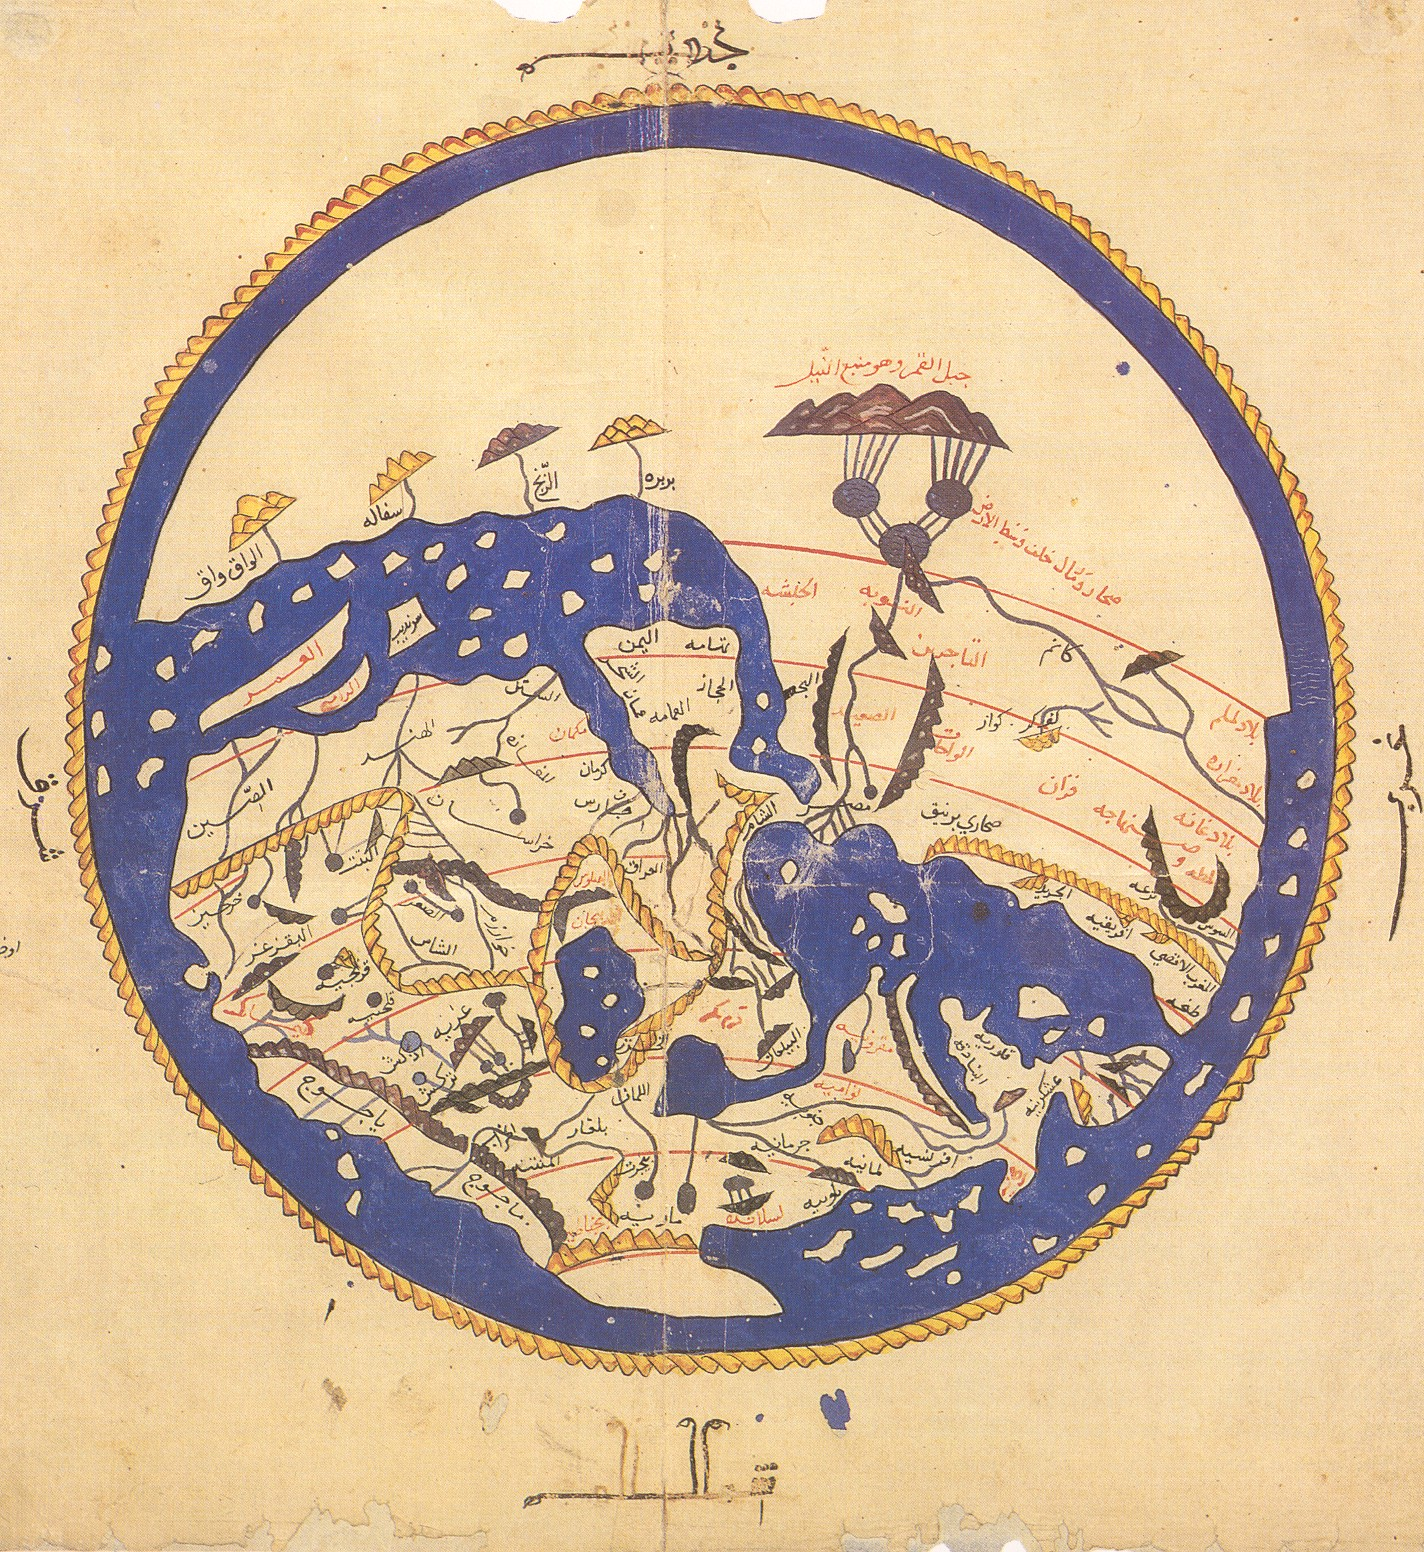
\includegraphics[width=1\textwidth]{figures/petaduniaalid.JPG}}
\caption{Gambaran pengantar peta dunia karya al-Idrisi tahun 1154.}
\end{figure}

\begin{figure}[ht]
	\centerline{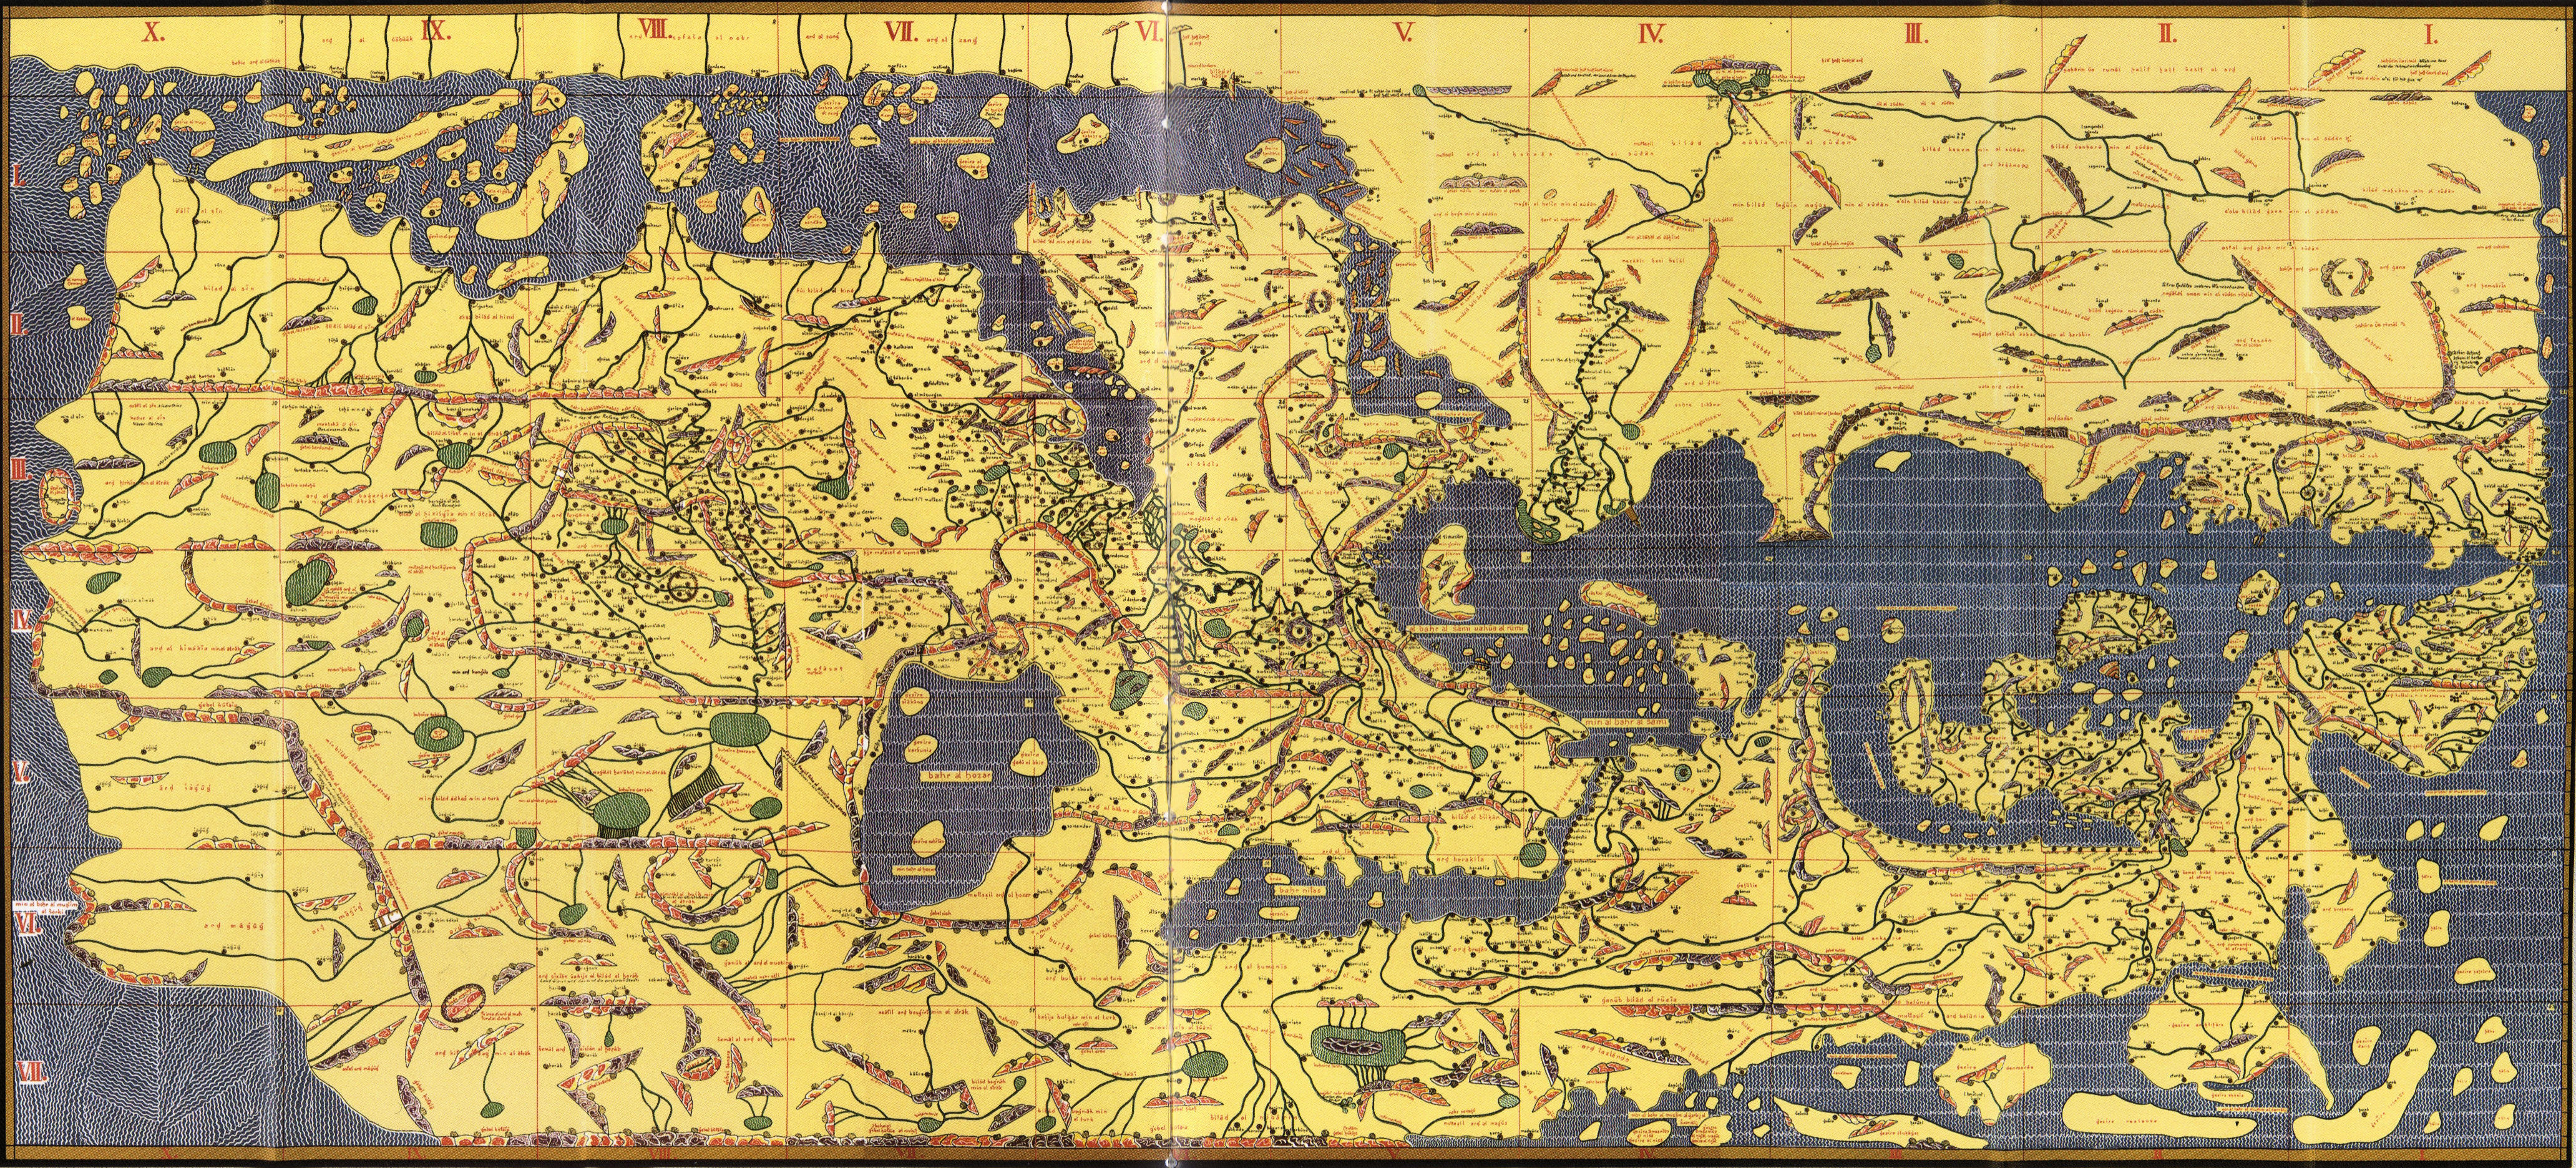
\includegraphics[width=1\textwidth]{figures/TabulaRogeriana.jpg}}
\vskip2pt
\caption{Tabula Rogeriana digambar oleh Al-Idrisi pada tahun 1154 untuk Raja Normandia Roger II dari Sisilia, setelah delapan menetap di istananya, di mana dia bekerja untuk penjelasan dan ilustrasi peta.}
\end{figure}

\section{Penentuan Kordinat}
Kordinat digunakan untuk mengacu sebuah titik lokasi di muka bumi, adapun beberapa jenis standar kordinat yang digunakan adalah.

\subsection{Kordinat Internasional}
Kordinat internasional dikenal dengan long dan lat.


\subsection{Kordinat Indonesia}
Masih ingatkah pelajaran geografi tentang letak Indonesia? maka kita bisa melihat jawaban tersebut dalam kordinat berbahasa indonesia.


	
\chapter[OS Semaphore]
{OS\\ Semaphore}
\section{System Operasi Semaphore}

	\subsection{Definisi}
	
		\begin{figure}[ht]
			\centerline{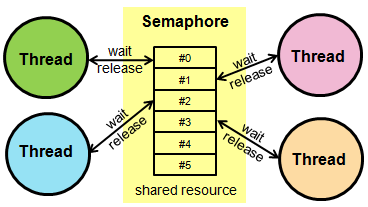
\includegraphics[width=0.5\textwidth]{figures/sema.png}}
			\caption{Semaphore}
			\label{sema}
			\end{figure}
	
		Semaphore merupakan salah satu teknik sinyal pada OS yang paling sederhana, dan merupakan konsep yang penting dalam OS desain, di mana nilai integer digunakan untuk memberi sinyal antar proses. 
		Hanya tiga operasi yang mungkin dilakukan pada semaphores, yang semuanya adalah atom: inisialisasi, keturunan, dan peningkatan. 
		Pengurangan operasi dapat menyebabkan proses yang diblokir, dan peningkatan operasi yang sedang berlangsung dapat mengakibatkan pemblokiran suatu proses. 
		Semaphore pada system operasi merupakan sebuah variabel bertipe integer. Di kehidupan nyata, semaphore merupakan sistem sinyal yang digunakan untuk memberi sinyal atau tanda dan berkomunikasi secara visual. 
		Semafor juga merupakan struktur data dalam bahasa komputer yang digunakan untuk menyinkronkan suatu proses, yaitu untuk memecahkan masalah di mana masalahnya lebih dari satu proses atau bisa 
		seperti thread yang akan dijalankan secara bersamaan dan harus diatur urutan kerja. Semaphore dibuat oleh Edsger Dijkstra dan pertama kali digunakan dalam sistem operasi.
		Nilai semaphore diinisialisasi dengan jumlah sumber daya yang dikontrol oleh pengguna. Dalam kasus khusus di mana ada sumber daya bersama, semaphore disebut semaphore biner. 
		Semaphore adalah solusi klasik dari dining philosophers problem, meskipun itu tidak mencegah deadlock.
		Pada software semaphore, semaphore merupakan variabel yang bertipe data integer tetapi tidak termasuk pada data yang sedang dilakukan inisialisasi, yang hanya dapat diakses melalui dua operasi standar, yaitu increment dan decrement. 
		Semaphore bisa digunakan untuk menyelesaikan masalah sinkronisasi secara umum, berdasarkan jenisnya. Semaphore hanya memiliki nilai 1 atau 0, atau lebih dari sama dengan 0. 
		Konsep semaphore pertama kali diajukan idenya oleh Edsger Dijkstra pada tahun 1967. Semaphore memiliki dua jenis, yaitu, Biner semaphore dan counting semaphore. 
		Biner semaphore tidak bisa memiliki semua jenis integer tetapi hanya memiliki 2 nilai yaitu 1 atau 0, Sering juga disebut sebagai semaphore primitive. Sedangkan Counting semaphore memiliki nilai 0, 1, sampai seterusnya atau integer lainnya. 
		Banyak sistem operasi yang tidak secara langsung menggunakan semaphore jenis ini, namun lebih banyak yang memanfaatkan semaphore jenis biner semaphore. 
		Pada semaphore ini harus diketahui bahwa, ada beberapa jenis dari counting semaphore yang salah satu jenisnya adalah semafor yang tidak bisa mencapai nilai negatif dan jenis yang lain adalah semaphore yang dapat mencapai nilai negatif. 
		Solusi dari Pembuatan Counting Semaphore adalah Binary Semaphore. Pembuatan counting semaphore banyak dilakukan para programmer untuk memenuhi alat sinkronisasi yang sesuai dengannya. 
		
		Operasi standarnya dalam bahasa pemrograman C :
		
		\begin{verbatim}
			void kunci(int sem_value) {
				while(sem_value <= 0);
				sem_value�;
			}
			void buka(int sem_value) {
				sem_value++;
			}
		\end{verbatim}
		
	\subsection{Prinsip Semaphore}
	
		\begin{enumerate}

			\item Suatu proses yang berbeda bisa berkaitan dengan memanfaatkan sinyal - sinyal.
			\item Suatu proses dapat dihentikan oleh proses yang lain.
			\item Semaphore bertipe data integer yang diakses oleh dua operasi atomik standar (wait dan signal).
			\item Ada dua operasi di semaphore (Down dan UP). Yang nama aslinya : P dan V.
		
		\end{enumerate}

	\subsection{Kelemahan Semaphore}
	
		\begin{enumerate}

			\item Semaphore termasuk Low Level.
			\item Dikarenakan semaphore tersebar di dalam seluruh program maka kita akan kesulitan dalam pemeliharaannya.
			\item Jika kita menghapus \"wait\" akan mengakibatkan \"nonmutual exclusion\".
			\item Jika kita menghapus \"signal\" akan mengakibatkan \"deadlock\".
			\item Jika terjadi deadlock akan sulit untuk dideteksi.

		\end{enumerate}
		
	\subsection{Semantik dan Impelementasi}
		Menghitung semaphores dilengkapi dengan dua operasi, secara historis dilambangkan sebagai P dan V (lihat § Nama operasi untuk nama alternatif). 
		Operasi V menambahkan semaphore S, dan operasi P menurunkannya.

		Nilai semaphore S adalah jumlah unit sumber daya yang saat ini tersedia. Operasi P membuang waktu atau tidur sampai sumber daya yang dilindungi oleh 
		semaphore menjadi tersedia, pada saat itu sumber daya segera diklaim. Operasi V adalah kebalikannya: ia membuat sumber daya tersedia lagi setelah proses
		selesai menggunakannya. Satu properti penting dari semaphore S adalah bahwa nilainya tidak dapat diubah kecuali dengan menggunakan operasi V dan P.

		Cara sederhana untuk memahami operasi tunggu (P) dan sinyal (V) adalah:
		
		\begin{itemize}
		
			\item menunggu: Jika nilai variabel semaphore tidak negatif, turunkan dengan 1. Jika variabel semaphore sekarang negatif, proses menunggu eksekusi 
			      diblokir (yaitu, ditambahkan ke antrian semaphore) sampai nilainya lebih besar atau sama dengan 1 Jika tidak, proses terus berjalan, setelah 
				  menggunakan satu unit sumber daya.
			\item sinyal: Menambah nilai semaphore variabel dengan 1. Setelah kenaikan, jika nilai pre-increment negatif (berarti ada proses menunggu sumber 
				  daya), ia mentransfer proses yang diblokir dari antrian menunggu semaphore ke antrean siap.
			
		\end{itemize}
		
		Banyak sistem operasi menyediakan primitif semaphore yang efisien yang membuka blokir proses menunggu ketika semaphore bertambah. Ini berarti bahwa proses tidak membuang waktu untuk memeriksa nilai semaphore yang tidak perlu.Konsep penghitungan semaphore dapat diperpanjang dengan kemampuan untuk mengklaim atau mengembalikan lebih dari satu \"unit\" dari semaphore, teknik yang diterapkan di Unix. Operasi V dan P yang dimodifikasi adalah sebagai berikut, menggunakan tanda kurung siku untuk menunjukkan operasi atom, yaitu operasi yang tampak terpisah dari perspektif proses lain:

		Semaphore pada system operasi merupakan sebuah variabel bertipe integer. Di kehidupan nyata, semaphore merupakan sistem sinyal yang digunakan untuk memberi sinyal atau tanda dan berkomunikasi secara visual. PPada software semaphore, semaphore merupakan variabel yang bertipe data integer tetapi tidak termasuk pada data yang sedang dilakukan inisialisasi, yang hanya dapat diakses melalui dua operasi standar, yaitu increment dan decrement. 
		Semaphore bisa digunakan untuk menyelesaikan masalah sinkronisasi secara umum, berdasarkan jenisnya. Semaphore hanya memiliki nilai 1 atau 0, atau lebih dari sama dengan 0. Konsep semaphore pertama kali diajukan idenya oleh Edsger Dijkstra pada tahun 1967. Semaphore memiliki dua jenis, yaitu, Biner semaphore dan counting semaphore. Biner semaphore hanya memiliki nilai 1 atau 0, Sering juga disebut sebagai semaphore primitive. Sedangkan Counting semaphore memiliki nilai 0, 1, sampai seterusnya atau integer lainnya. Banyak sistem operasi yang tidak secara langsung menggunakan semaphore jenis ini, namun lebih banyak yang memanfaatkan semaphore jenis biner semaphore

	
	\subsection{Prinsip Semaphore}
		\begin{enumerate}

			\item Suatu proses yang berbeda bisa berkaitan dengan memanfaatkan sinyal - sinyal.
			\item Suatu proses dapat dihentikan oleh proses lainnya.
			\item Semaphore bertipe data integer yang diakses oleh dua operasi atomik standar (wait dan signal).
			\item Ada dua operasi di semaphore (Down dan UP). Yang nama aslinya : P dan V.
			
		\end{enumerate}
		
	\subsection{Kelemahan Semaphore}

		\begin{enumerate}

			\item Semaphore termasuk Low Level.
			\item Dikarenaka semaphore tersebar di dalam seluruh program maka kita akan kesulitan dalam pemeliharaannya.
			\item Jika kita menghapus \"wait\" akan mengakibatkan \"nonmutual exclusion\".
			\item Jika kita menghapus \"signal\" akan mengakibatkan \"deadlock\".
			\item Jika terjadi deadlock akan sulti untuk dideteksi.
			
		\begin{enumerate}
		
	\cite{luu1982apparatus}
	\cite{lauesen1975large}
	\cite{hoare1974monitors}


\chapter[Proses OS]
{OS\\ Proses}
%kelompok 1 Sistem Operasi (Proses Os)
%Kelas D4 TI 1B
%Adam Noer Hidayatullah 1174097
%Ichsan Hizman
%Teddy
%Nisrina Aulia
%Irvan Rizkiansyah 1174043

\section{proses}

	\subsection{Proses}	
	Proses adalah sebuah  program yang sedang dieksekusi. Sedangkan program idalah merupakan kumpulan-kumpulan  dari suatu  instruksi yang sudah ditulis ke dalam bahasa yang dapat  dimengerti oleh sistem operasi.Proses berisi tentang sebuah instruksi dan sebuah data. program counter dan seluruh register pemroses, stack ini  berisi data sementara contohnya seperti alamat pengiriman, parameter rutin dan variabel lokal. Sistem operasi diharuskan untuk mengelola semua proses di dalam sistem tersebut dan mengalokasikan sumber daya ke sebuah  proses-proses sesuai dengan kebijaksanaan untuk memenuhi sasaran sistem
	
	\subsection{Istilah yang berkaitan dengan proses}
		\begin{itemize}
			\item Multiprogramming
			Multiprogramming (multitasking) adalah  istilah teknologi informasi dengan mengunakan bahasa inggris yang baik  mengacup kepada sebuah metode dimana banyak sebuah pekerjaan atau yang dikenal juga sebagai proses  dengan diolah dengan menggunakan sumber daya CPU yang sama.
			Contohnya sistem operasi jenis ini antaranya linux dan windows.
			\item Multiprocessing
			kemampuan komputer untuk melakukan beberapa proses dengan waktu yang bersamaan, dibantu dengan keberadaan teknologi yang berbasis multiprocessor.
			Contohnya seperti computer server.
			\item Distributed processing/computing
			Mengerjakan semua proses pengolahan data secara bersamaan antara komputer pusat dengan beberapa komputer yang lebih kecil dan saling berhubungan denan melalui jalur komunikasi.
			Contohnya komputer yang dirancang untuk melaksanakan tugas-tugas proyek.
		\end{itemize}
		
	\subsection{Fungsi fungsi sistem operasi}
		\begin{enumerate}
			\item Resource manager, pengolahan sumber daya dan mengalokasikan.
			\item Interface atau tatap muka, sebagai perantara antara pengguna dengan perangkat keras.
			\item Coordinator, mengkoordinasi fasilitas sehingga aktifitas yang komplek dapat diatur..
		\end{enumerate}
		
		\subsection{jenis jenis sistem operasi pada komputer}
			\begin{enumerate}
				\item Windows, merupakan pengembangan dari sistem operasi DOS. windows juga mudah untuk dipelajari.
				\item Mac OS, merupakan sistem operasi yang diciptakan oleh Apple. Mac OS memiliki tingkat keamanan yang tinggi.
				\item Linux, memiliki kestabilan yang baik, yang sering digunakan sebagai sistem operasi pada server.
				\item Android, merupakan sistem operasi pada smartphone. android sama seperti Linux, yaitu mudah dikembangkan.
			\end{enumerate}
			
	\subsection{Status proses}
	Terdapat 5 macam jenis status yang mungkin dimiliki oleh suatu proses :
	\begin{enumerate}
		\item New, yaitu status yang dimiliki pada saat proses baru saja terjadi.
		\item Ready, yaitu status dimana proses siap untuk dieksekusi pada giliran berikutnya.
		\item Running, yaitu status suatu proses dimana saat ini proses tersebut sedang dieksekusi oleh prosesor
		\item Waiting, yaitu status dimana proses yang tidak bisa dijalankan di saat prosesor sudah siap, status yang dimiliki pada saat proses menunggu suatu sebuah event seperti I/O
		\item Terminated, yaitu status yang dimiliki pada saat proses telah selesai dieksekusi
	\end{enumerate}
	
	Berikut ini adalah proses dari ke-5 status proses di atas :
	\begin{enumerate}
		\item New ke Ready
		Pertama Status dibuat lalu setelah itu , status akan memasuki proses ready dan siap untuk memasuki proses selanjutnya.
		\item Ready ke running
		Di saat sedang memilih proses yang akan dioperasikan, sistem operasi akan memilih salah satu proses yang berada didalam keadaan status ready.
		\item Running ke waiting
		Suatu proses dimasukkan dalam keadaan status waiting jika proses itu meminta sesuatu yang dapat menyebabkannya harus menunggu. Sebuah request ke sistem operasi yang pada umumnya merupakan bentuk panggilan dari layanan sistem (panggilan dari program yang sedang beroperasi ke dalam suatu prosedur yang merupakan bagian kode sistem operasi) misalnya seperti sebuah proses yang bisa meminta suatu layanan dari sistem operasi yang tidak siap dilakukan oleh sistem opersi dengan segera. Atau proses yang bisa menginisiasi suatu aksi, seperti misalnya operasi I/O, yang seharusnya bisa diselesaikan sebelum proses itu melanjutkan operasinya. Pada saat proses saling melakukan komunikasi dengan proses yang lainnya, suatu proses bisa diblokir jika sedang menunggu proses lainnya untuk menyediakan input.
		\item Running ke ready
		Pada umumnya alasan transisi ini ialah dimana sebuah proses yang lagi berjalan sudah mencapai batas waktu maksimum yang telah diizinkan bagi instruksi yang tidak diinterupsi. Terdapat beberapa alasan yang menyebabkan transisi ini terjadi, yang tidak diimplementasikan oleh setiap sistem operasi. Misalnya apabila sistem operasi meng-assign tingkat prioritas yang berbeda pada beberapa proses yang berlainan, suatu proses bisa diambil lebih dulu.
		\item Waiting ke ready
		Apabila suatu proses dalam keadaan status waiting sudah selesai dalam mendapatkan sumber daya, seperti file atau bagian virtual memori bagi pakai atau juga sudah selesai setelah menunggu proses yang lainnya untuk menyediakan input atau sudah selesai dalam menunggu pesan lainnya.
		\item Runing ke finish(terminated)
		proses yang sedang berjalan dihentikan oleh Sistem Operasi jika proses itu telah selesai atau tidak jadi dieksekusi. Hal ini terjadi dikarenakan jika proses induknya sendiri telah berhenti.
	\end{enumerate}
	
	Dan berikut ini adalah diagram dari ke-5 status proses tadi :
	
	\begin{figure} [ht]
	\centerline{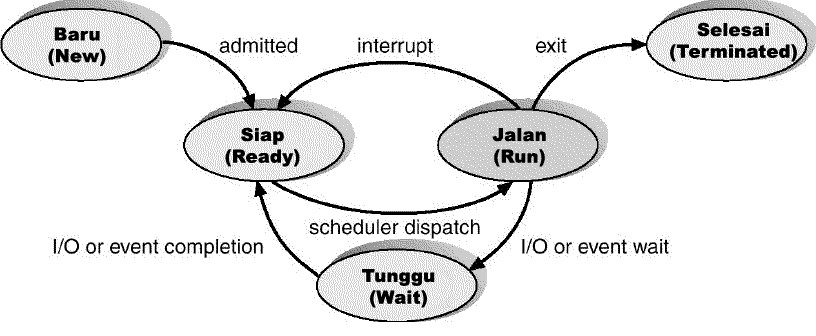
\includegraphics[width=1\textwidth]{figures/statusproses.jpg}}
	\caption{Gambar Status Proses}
	\label{statusproses}
	\end{figure}
	
	\ref{statusproses}
	
	\subsection{Contoh dari status proses}
	Setiap proses pasti mempunyai status yang harus diperhatikan oleh sistem operasi yang akan dicatat dalam berbagai macam tabel yang saling berhubungan, yaitu :
		\begin{itemize}
			\item Tabel informasi manajemen memori, Digunakan untuk menjaga keutuhan dari suatu memori utama dan memori sekunder yang akan menyimpan suatu informasi.
			\item Tabel informasi manajemen masukan atau keluaran, Digunakan untuk melakukan pengelolan sebuah perangkat masukan atau keluaran, yang dimana perangkat tersebut akan digunakan oleh proses yang tertentu, sehingga harus dijaga supaya proses yang lainnya tidak akan memakainya. Sistem operasi harus mengetahui status operasi masukan atau keluaran dan lokasi suatu memori utama yang akan digunakan untuk melakukan transfer data.
			\item Tabel informasi sistem file, Tabel dimana yang berisikan mengenai informasi lokasi pada memori sekunder, informasi ekstensi file, informasi status pada saat itu dan menyimpan atribut-atribut file yang lainnya.
			\item Tabel proses, Digunakan untuk mengelola informasi suatu proses pada sistem operasi, yang berlokasi di memori, atribut proses dan status lainnya.
		\end{itemize}
	
	\subsection{Proses Control Block/Blocked}
	Sebuah struktur data yang dipakai oleh Sistem Operasi untuk mengelola sebuah proses. Hampir semua Sistem Operasi yang modern telah menggunakan PCB (Process Control Block) namun strukturnya yang berbeda-beda pada setiap Sistem Operasi tersebut. PCB (Process Control Block) juga memiliki informasi yang berhubungan dengan proses, ialah: tanda pengenal bagi sebuah proses (Process ID) yang sangat unik dan akan menjadi status proses, nomor identitas, prioritas eksekusi proses dan semua informasi lokasi proses dalam memori. Prioritas yang dimiliki oleh sebuah proses merupakan sebuah nilai atau besaran yang akan menunjukkan seberapa sering proses harus dieksekusi oleh prosesor. Sebuah proses yang mempunyai nilai prioritas yang cenderung lebih tinggi, akan lebih sering dieksekusi atau dieksekusi terlebih dulu jika dibandingkan dengan proses yang mempunyai prioritas yang lebih rendah.
	Sebuah PCB (Process Control Block) ditunjukkan dalam tabel berikut : 
	
	\begin{table}[H]
		\begin{tabular}{|c|c|}
			\hline
			Pointer & State Proses\\
			\hline
			\multicolumn{2}{|c|}{Nomor Proses}\\
			\hline
			\multicolumn{2}{|c|}{Program Counter}\\
			\hline
			\multicolumn{2}{|c|}{Registers}\\
			\hline
			\multicolumn{2}{|c|}{Batas Memori}\\
			\hline
			\multicolumn{2}{|c|}{Daftar berkas yang telah dibuka}\\
			\hline
			\multicolumn{2}{|c|}{.......}\\
		\end{tabular}
	\end{table}
	
	PCB dibagi menjadi 3 kelompok yaitu :
	\begin{itemize}
		\item Process identification data
		pasti akan selalu mengikut-sertakan suatu identifier yang sangat unik untuk prosesnya (hampir selalu mempunyai nilai integer) dan pada sebuah sistem multiuser-multitasking, data yang contohnya seperti identifier grup pengguna, identifier proses, identifier pengguna, dan yang lainnya. Proses ini sangat relevan, karena itu sering dipakai untuk referensi silang tabel sistem operasi, misalnya seperti memungkinkan untuk mengidentifikasi sebuah proses yang menggunakan device I/O, atau daerah memori.
		\item Processor state data
		potongan-potongan dari informasi yang mengartidefinisikan status dari sebuah proses ketika proses tersebut ditangguhkan, dan memungkinkan sistem operasi untuk melakukan restart proses pada akhirnya dan akan masih dapat mengeksekusinya dengan benar. Hal ini akan selalu mengikut-sertakan isi dari register CPU tujuan.
		\item Process control data
		digunakan oleh sistem operasi untuk mengelola proses itu sendiri.
	\end{itemize}
Dirangkum dari makalah \cite{apriyanto2009sistem}
Dirangkum dari makalah \cite{silberschatz2014operating}

%{OS\\ Proses OS}
%%kelompok 1 Sistem Operasi (Proses Os)
%Kelas D4 TI 1B
%Adam Noer Hidayatullah 1174097
%Ichsan Hizman
%Teddy
%Nisrina Aulia
%Irvan Rizkiansyah 1174043

\section{proses}

	\subsection{Proses}	
	Proses adalah sebuah  program yang sedang dieksekusi. Sedangkan program idalah merupakan kumpulan-kumpulan  dari suatu  instruksi yang sudah ditulis ke dalam bahasa yang dapat  dimengerti oleh sistem operasi.Proses berisi tentang sebuah instruksi dan sebuah data. program counter dan seluruh register pemroses, stack ini  berisi data sementara contohnya seperti alamat pengiriman, parameter rutin dan variabel lokal. Sistem operasi diharuskan untuk mengelola semua proses di dalam sistem tersebut dan mengalokasikan sumber daya ke sebuah  proses-proses sesuai dengan kebijaksanaan untuk memenuhi sasaran sistem
	
	\subsection{Istilah yang berkaitan dengan proses}
		\begin{itemize}
			\item Multiprogramming
			Multiprogramming (multitasking) adalah  istilah teknologi informasi dengan mengunakan bahasa inggris yang baik  mengacup kepada sebuah metode dimana banyak sebuah pekerjaan atau yang dikenal juga sebagai proses  dengan diolah dengan menggunakan sumber daya CPU yang sama.
			Contohnya sistem operasi jenis ini antaranya linux dan windows.
			\item Multiprocessing
			kemampuan komputer untuk melakukan beberapa proses dengan waktu yang bersamaan, dibantu dengan keberadaan teknologi yang berbasis multiprocessor.
			Contohnya seperti computer server.
			\item Distributed processing/computing
			Mengerjakan semua proses pengolahan data secara bersamaan antara komputer pusat dengan beberapa komputer yang lebih kecil dan saling berhubungan denan melalui jalur komunikasi.
			Contohnya komputer yang dirancang untuk melaksanakan tugas-tugas proyek.
		\end{itemize}
		
	\subsection{Fungsi fungsi sistem operasi}
		\begin{enumerate}
			\item Resource manager, pengolahan sumber daya dan mengalokasikan.
			\item Interface atau tatap muka, sebagai perantara antara pengguna dengan perangkat keras.
			\item Coordinator, mengkoordinasi fasilitas sehingga aktifitas yang komplek dapat diatur..
		\end{enumerate}
		
		\subsection{jenis jenis sistem operasi pada komputer}
			\begin{enumerate}
				\item Windows, merupakan pengembangan dari sistem operasi DOS. windows juga mudah untuk dipelajari.
				\item Mac OS, merupakan sistem operasi yang diciptakan oleh Apple. Mac OS memiliki tingkat keamanan yang tinggi.
				\item Linux, memiliki kestabilan yang baik, yang sering digunakan sebagai sistem operasi pada server.
				\item Android, merupakan sistem operasi pada smartphone. android sama seperti Linux, yaitu mudah dikembangkan.
			\end{enumerate}
			
	\subsection{Status proses}
	Terdapat 5 macam jenis status yang mungkin dimiliki oleh suatu proses :
	\begin{enumerate}
		\item New, yaitu status yang dimiliki pada saat proses baru saja terjadi.
		\item Ready, yaitu status dimana proses siap untuk dieksekusi pada giliran berikutnya.
		\item Running, yaitu status suatu proses dimana saat ini proses tersebut sedang dieksekusi oleh prosesor
		\item Waiting, yaitu status dimana proses yang tidak bisa dijalankan di saat prosesor sudah siap, status yang dimiliki pada saat proses menunggu suatu sebuah event seperti I/O
		\item Terminated, yaitu status yang dimiliki pada saat proses telah selesai dieksekusi
	\end{enumerate}
	
	Berikut ini adalah proses dari ke-5 status proses di atas :
	\begin{enumerate}
		\item New ke Ready
		Pertama Status dibuat lalu setelah itu , status akan memasuki proses ready dan siap untuk memasuki proses selanjutnya.
		\item Ready ke running
		Di saat sedang memilih proses yang akan dioperasikan, sistem operasi akan memilih salah satu proses yang berada didalam keadaan status ready.
		\item Running ke waiting
		Suatu proses dimasukkan dalam keadaan status waiting jika proses itu meminta sesuatu yang dapat menyebabkannya harus menunggu. Sebuah request ke sistem operasi yang pada umumnya merupakan bentuk panggilan dari layanan sistem (panggilan dari program yang sedang beroperasi ke dalam suatu prosedur yang merupakan bagian kode sistem operasi) misalnya seperti sebuah proses yang bisa meminta suatu layanan dari sistem operasi yang tidak siap dilakukan oleh sistem opersi dengan segera. Atau proses yang bisa menginisiasi suatu aksi, seperti misalnya operasi I/O, yang seharusnya bisa diselesaikan sebelum proses itu melanjutkan operasinya. Pada saat proses saling melakukan komunikasi dengan proses yang lainnya, suatu proses bisa diblokir jika sedang menunggu proses lainnya untuk menyediakan input.
		\item Running ke ready
		Pada umumnya alasan transisi ini ialah dimana sebuah proses yang lagi berjalan sudah mencapai batas waktu maksimum yang telah diizinkan bagi instruksi yang tidak diinterupsi. Terdapat beberapa alasan yang menyebabkan transisi ini terjadi, yang tidak diimplementasikan oleh setiap sistem operasi. Misalnya apabila sistem operasi meng-assign tingkat prioritas yang berbeda pada beberapa proses yang berlainan, suatu proses bisa diambil lebih dulu.
		\item Waiting ke ready
		Apabila suatu proses dalam keadaan status waiting sudah selesai dalam mendapatkan sumber daya, seperti file atau bagian virtual memori bagi pakai atau juga sudah selesai setelah menunggu proses yang lainnya untuk menyediakan input atau sudah selesai dalam menunggu pesan lainnya.
		\item Runing ke finish(terminated)
		proses yang sedang berjalan dihentikan oleh Sistem Operasi jika proses itu telah selesai atau tidak jadi dieksekusi. Hal ini terjadi dikarenakan jika proses induknya sendiri telah berhenti.
	\end{enumerate}
	
	Dan berikut ini adalah diagram dari ke-5 status proses tadi :
	
	\begin{figure} [ht]
	\centerline{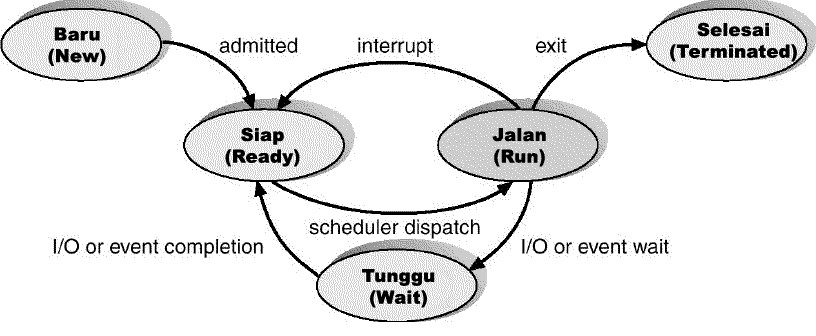
\includegraphics[width=1\textwidth]{figures/statusproses.jpg}}
	\caption{Gambar Status Proses}
	\label{statusproses}
	\end{figure}
	
	\ref{statusproses}
	
	\subsection{Contoh dari status proses}
	Setiap proses pasti mempunyai status yang harus diperhatikan oleh sistem operasi yang akan dicatat dalam berbagai macam tabel yang saling berhubungan, yaitu :
		\begin{itemize}
			\item Tabel informasi manajemen memori, Digunakan untuk menjaga keutuhan dari suatu memori utama dan memori sekunder yang akan menyimpan suatu informasi.
			\item Tabel informasi manajemen masukan atau keluaran, Digunakan untuk melakukan pengelolan sebuah perangkat masukan atau keluaran, yang dimana perangkat tersebut akan digunakan oleh proses yang tertentu, sehingga harus dijaga supaya proses yang lainnya tidak akan memakainya. Sistem operasi harus mengetahui status operasi masukan atau keluaran dan lokasi suatu memori utama yang akan digunakan untuk melakukan transfer data.
			\item Tabel informasi sistem file, Tabel dimana yang berisikan mengenai informasi lokasi pada memori sekunder, informasi ekstensi file, informasi status pada saat itu dan menyimpan atribut-atribut file yang lainnya.
			\item Tabel proses, Digunakan untuk mengelola informasi suatu proses pada sistem operasi, yang berlokasi di memori, atribut proses dan status lainnya.
		\end{itemize}
	
	\subsection{Proses Control Block/Blocked}
	Sebuah struktur data yang dipakai oleh Sistem Operasi untuk mengelola sebuah proses. Hampir semua Sistem Operasi yang modern telah menggunakan PCB (Process Control Block) namun strukturnya yang berbeda-beda pada setiap Sistem Operasi tersebut. PCB (Process Control Block) juga memiliki informasi yang berhubungan dengan proses, ialah: tanda pengenal bagi sebuah proses (Process ID) yang sangat unik dan akan menjadi status proses, nomor identitas, prioritas eksekusi proses dan semua informasi lokasi proses dalam memori. Prioritas yang dimiliki oleh sebuah proses merupakan sebuah nilai atau besaran yang akan menunjukkan seberapa sering proses harus dieksekusi oleh prosesor. Sebuah proses yang mempunyai nilai prioritas yang cenderung lebih tinggi, akan lebih sering dieksekusi atau dieksekusi terlebih dulu jika dibandingkan dengan proses yang mempunyai prioritas yang lebih rendah.
	Sebuah PCB (Process Control Block) ditunjukkan dalam tabel berikut : 
	
	\begin{table}[H]
		\begin{tabular}{|c|c|}
			\hline
			Pointer & State Proses\\
			\hline
			\multicolumn{2}{|c|}{Nomor Proses}\\
			\hline
			\multicolumn{2}{|c|}{Program Counter}\\
			\hline
			\multicolumn{2}{|c|}{Registers}\\
			\hline
			\multicolumn{2}{|c|}{Batas Memori}\\
			\hline
			\multicolumn{2}{|c|}{Daftar berkas yang telah dibuka}\\
			\hline
			\multicolumn{2}{|c|}{.......}\\
		\end{tabular}
	\end{table}
	
	PCB dibagi menjadi 3 kelompok yaitu :
	\begin{itemize}
		\item Process identification data
		pasti akan selalu mengikut-sertakan suatu identifier yang sangat unik untuk prosesnya (hampir selalu mempunyai nilai integer) dan pada sebuah sistem multiuser-multitasking, data yang contohnya seperti identifier grup pengguna, identifier proses, identifier pengguna, dan yang lainnya. Proses ini sangat relevan, karena itu sering dipakai untuk referensi silang tabel sistem operasi, misalnya seperti memungkinkan untuk mengidentifikasi sebuah proses yang menggunakan device I/O, atau daerah memori.
		\item Processor state data
		potongan-potongan dari informasi yang mengartidefinisikan status dari sebuah proses ketika proses tersebut ditangguhkan, dan memungkinkan sistem operasi untuk melakukan restart proses pada akhirnya dan akan masih dapat mengeksekusinya dengan benar. Hal ini akan selalu mengikut-sertakan isi dari register CPU tujuan.
		\item Process control data
		digunakan oleh sistem operasi untuk mengelola proses itu sendiri.
	\end{itemize}
Dirangkum dari makalah \cite{apriyanto2009sistem}
Dirangkum dari makalah \cite{silberschatz2014operating}

\chapter[Sistem Operasi]
{OS\\ Sistem Operasi}
\section{Sistem Operasi}
	\subsection{Definisi}
		\begin{enumerate}
			\item Sistem operasi (OS) adalah sistem perangkat lunak yang mengelola hardware dan sumber daya perangkat lunak dengan menyediakan pelayanan secara umum untuk program komputer.

			\item Sistem operasi berbagi waktu menjadwalkan tugas untuk penggunaan sistem yang efisien dan mungkin juga termasuk perangkat lunak akuntansi untuk alokasi biaya waktu prosesor, penyimpanan massal, pencetakan, dan sumber daya lainnya.
			\item Untuk fungsi perangkat keras seperti input dan output dan alokasi memori, sistem operasi bertindak sebagai perantara antara program dan perangkat keras komputer, meskipun kode aplikasi biasanya dijalankan langsung oleh perangkat keras dan sering membuat panggilan sistem ke fungsi OS atau terganggu oleh saya t. Sistem operasi banyak ditemukan pada perangkat komputer,telepon seluler dan konsol permainan video ke server web dan superkomputer.

			\item Sistem operasi berbagi waktu menjadwalkan tugas untuk penggunaan sistem yang efisien dan mungkin juga termasuk perangkat lunak akuntansi untuk alokasi biaya waktu prosesor, penyimpanan massal, pencetakan, dan sumber daya lainnya.
			\item Untuk fungsi perangkat keras seperti input dan output dan alokasi memori, sistem operasi bertindak sebagai perantara antara program dan perangkat keras komputer, meskipun kode aplikasi biasanya dijalankan langsung oleh perangkat keras dan sering membuat panggilan sistem ke fungsi OS atau terganggu oleh saya t. Sistem operasi banyak ditemukan pada perangkat komputer,telepon seluler dan konsol permainan video ke server web dan superkomputer.

			\item Sistem operasi desktop yang dominan adalah Microsoft Windows dengan pangsa pasar sekitar 82,74%. macOS oleh Apple Inc. berada di tempat kedua (13,23%), dan varietas Linux secara kolektif berada di tempat ketiga (1,57%). Di sektor seluler (gabungan ponsel dan tablet), penggunaan pada tahun 2017 adalah hingga 70% dari Google Android dan menurut data kuartal ketiga 2016, Android pada smartphone dominan dengan 87,5 persen dan tingkat pertumbuhan 10,3 persen per tahun, diikuti oleh Apple iOS dengan 12,1 persen dan penurunan per tahun di pangsa pasar 5,2 persen, sementara jumlah sistem operasi lainnya hanya 0,3 persen. Distribusi Linux dominan di sektor server dan superkomputer. Kelas khusus lainnya dari sistem operasi, seperti embedded dan sistem real-time, ada untuk banyak aplikasi.
		\end{enumerate}
	\begin{figure}[ht]
		\centerline{
\includegraphics[width=1\textwidth]{figures/OS.JPG}}
		\caption{Sistem Operasi}
		\label{OS}
	\end{figure}

\subsection{Jenis sistem operasi}
\subsubsection{Single dan multi-tasking}
	\begin{enumerate}
		\item Sistem satu tugas hanya dapat menjalankan satu program dalam satu waktu, sementara sistem operasi multi-tasking memungkinkan lebih dari satu program berjalan dalam konkurensi. Ini dicapai dengan time-sharing, di mana waktu prosesor yang tersedia dibagi antara beberapa proses. Proses ini masing-masing terganggu berulang kali dalam irisan waktu oleh subsistem penjadwalan tugas dari sistem operasi. Multi-tasking dapat dicirikan dalam tipe preemptif dan kooperatif. Dalam preemptive multitasking, sistem operasi memotong waktu CPU dan mendedikasikan slot untuk masing-masing program. Sistem operasi mirip Unix, seperti Solaris dan Linux — serta non-Unix-like, seperti AmigaOS — mendukung multitasking preemptif. Multitasking kooperatif dicapai dengan mengandalkan pada setiap proses untuk menyediakan waktu untuk proses lain dengan cara yang ditentukan. Versi 16-bit Microsoft Windows menggunakan multi-tasking kooperatif. Versi 32-bit dari Windows NT dan Win9x, menggunakan preemptive multi-tasking.
	\end{enumerate}
\subsection{Single dan multi-user}
	\begin{enumerate}
		\item 1. Sistem operasi pengguna tunggal tidak memiliki fasilitas untuk membedakan pengguna, tetapi dapat memungkinkan beberapa program berjalan bersama-sama. Sistem operasi multi-pengguna memperluas konsep dasar multi-tasking dengan fasilitas yang mengidentifikasi proses dan sumber daya, seperti ruang disk, milik beberapa pengguna, dan sistem memungkinkan banyak pengguna untuk berinteraksi dengan sistem pada saat yang bersamaan. 
		\item 2. Sistem operasi berbagi waktu menjadwalkan tugas untuk penggunaan sistem yang efisien dan mungkin juga termasuk perangkat lunak akuntansi untuk alokasi biaya waktu prosesor, penyimpanan massal, pencetakan, dan sumber daya lainnya untuk banyak pengguna.
	\end{enumerate}
\subsection{Pendistribusian}
	\begin{enumerate}
		\item Sistem operasi terdistribusi mengelola sekelompok komputer yang berbeda dan membuatnya tampak sebagai komputer tunggal. Pengembangan jaringan komputer yang dapat dihubungkan dan berkomunikasi satu sama lain menimbulkan komputasi terdistribusi. Komputasi terdistribusi dilakukan pada lebih dari satu mesin. Ketika komputer dalam kelompok bekerja dalam kerja sama, mereka membentuk sistem terdistribusi.
	\end{enumerate}
\subsection{Sejarah}
	\begin{enumerate}
		\item Komputer awal dibangun untuk melakukan serangkaian tugas tunggal, seperti kalkulator. Fitur-fitur sistem operasi dasar dikembangkan pada tahun 1950-an, seperti fungsi monitor penduduk yang dapat secara otomatis menjalankan program yang berbeda secara berurutan untuk mempercepat pemrosesan. Sistem operasi tidak ada dalam bentuk modern dan lebih kompleks hingga awal 1960-an. Fitur perangkat keras ditambahkan, yang memungkinkan penggunaan pustaka runtime, interupsi, dan pemrosesan paralel. Ketika komputer pribadi menjadi populer pada tahun 1980-an, sistem operasi dibuat untuk mereka yang serupa dalam konsep untuk yang digunakan pada komputer yang lebih besar.

		\item Pada 1940-an, sistem digital elektronik paling awal tidak memiliki sistem operasi. Sistem elektronik saat ini diprogram pada deretan switch mekanis atau oleh kabel jumper pada papan steker. Ini adalah sistem tujuan khusus yang, misalnya, menghasilkan tabel balistik untuk militer atau mengontrol pencetakan cek gaji dari data pada kartu kertas berlubang. Setelah komputer tujuan umum yang dapat diprogram diciptakan, bahasa mesin (terdiri dari string digit biner 0 dan 1 pada pita kertas berlubang) diperkenalkan yang mempercepat proses pemrograman.
		\item Pada awal 1950-an, komputer hanya dapat menjalankan satu program dalam satu waktu. Setiap pengguna memiliki satu-satunya penggunaan komputer untuk jangka waktu terbatas dan akan tiba pada waktu yang dijadwalkan dengan program dan data pada kartu kertas berlubang atau pita berlubang. Program akan dimuat ke dalam mesin, dan mesin akan diatur untuk bekerja sampai program selesai atau crash. Program umumnya dapat di-debug melalui panel depan menggunakan saklar beralih dan lampu panel. Dikatakan bahwa Alan Turing adalah seorang ahli dalam mesin Manchester Mark 1 awal ini, dan dia sudah mendapatkan konsep primitif dari sistem operasi dari prinsip-prinsip mesin Turing universal.
		\item Kemudian mesin datang dengan perpustakaan program, yang akan dikaitkan dengan program pengguna untuk membantu dalam operasi seperti input dan output dan menghasilkan kode komputer dari kode simbolik yang dapat dibaca manusia. Ini adalah awal dari sistem operasi modern. Namun, mesin masih menjalankan pekerjaan tunggal pada suatu waktu. Di Cambridge University di Inggris, antrian pekerjaan pada suatu waktu adalah garis pencucian (garis pakaian) dari mana kaset digantung dengan pakaian warna berbeda untuk menunjukkan prioritas pekerjaan. 

		\item Pada 1940-an, sistem digital elektronik paling awal tidak memiliki sistem operasi. Sistem elektronik saat ini diprogram pada deretan switch mekanis atau oleh kabel jumper pada papan steker. Ini adalah sistem tujuan khusus yang, misalnya, menghasilkan tabel balistik untuk militer atau mengontrol pencetakan cek gaji dari data pada kartu kertas berlubang. Setelah komputer tujuan umum yang dapat diprogram diciptakan, bahasa mesin (terdiri dari string digit biner 0 dan 1 pada pita kertas berlubang) diperkenalkan yang mempercepat proses pemrograman.
		\item Pada awal 1950-an, komputer hanya dapat menjalankan satu program dalam satu waktu. Setiap pengguna memiliki satu-satunya penggunaan komputer untuk jangka waktu terbatas dan akan tiba pada waktu yang dijadwalkan dengan program dan data pada kartu kertas berlubang atau pita berlubang. Program akan dimuat ke dalam mesin, dan mesin akan diatur untuk bekerja sampai program selesai atau crash. Program umumnya dapat di-debug melalui panel depan menggunakan saklar beralih dan lampu panel. Dikatakan bahwa Alan Turing adalah seorang ahli dalam mesin Manchester Mark 1 awal ini, dan dia sudah mendapatkan konsep primitif dari sistem operasi dari prinsip-prinsip mesin Turing universal.
		\item Kemudian mesin datang dengan perpustakaan program, yang akan dikaitkan dengan program pengguna untuk membantu dalam operasi seperti input dan output dan menghasilkan kode komputer dari kode simbolik yang dapat dibaca manusia. Ini adalah awal dari sistem operasi modern. Namun, mesin masih menjalankan pekerjaan tunggal pada suatu waktu. Di Cambridge University di Inggris, antrian pekerjaan pada suatu waktu adalah garis pencucian (garis pakaian) dari mana kaset digantung dengan pakaian warna berbeda untuk menunjukkan prioritas pekerjaan. 

	\end{enumerate}
\subsection{Mikrokomputer}
	\begin{enumerate}
		\item Mikrokomputer pertama tidak memiliki kapasitas atau kebutuhan untuk sistem operasi yang rumit yang telah dikembangkan untuk mainframe dan miniis, sistem operasi minimalis dikembangkan, sering dimuat dari ROM dan dikenal sebagai monitor. Salah satu sistem operasi disk awal yang terkenal adalah CP / M, yang didukung oleh banyak mikrokomputer awal dan sangat ditiru oleh Microsoft MS-DOS, yang menjadi sangat populer sebagai sistem operasi yang dipilih untuk PC IBM . Pada 1980-an, Apple Computer Inc.  meninggalkan seri mikrokomputer Apple II yang populer untuk memperkenalkan komputer Apple Macintosh dengan antarmuka pengguna grafis inovatif  ke Mac OS.

		\item Pengenalan chip CPU Intel 80386 pada bulan Oktober 1985,  dengan arsitektur 32-bit dan kemampuan paging, menyediakan komputer pribadi dengan kemampuan untuk menjalankan sistem operasi multitasking seperti komputer minikomputer dan mainframe sebelumnya. Microsoft merespon perkembangan ini dengan mempekerjakan Dave Cutler, yang telah mengembangkan sistem operasi VMS untuk Digital Equipment Corporation. Dia dijadikan pemimpin dalam proses  pengembangan sistem operasi Windows NT, yang terus-menerus berfungsi sebagai dasar untuk jalur/way sistem operasi Microsoft. Steve Jobs, co-founder Apple Inc., memulai NeXT Computer Inc., yang mengembangkan sistem operasi NEXTSTEP. NEXTSTEP nantinya akan diakuisisi oleh Apple Inc. dan digunakan, bersama dengan kode dari FreeBSD sebagai inti dari Mac OS X.

		\item Pengenalan chip CPU Intel 80386 pada bulan Oktober 1985,  dengan arsitektur 32-bit dan kemampuan paging, menyediakan komputer pribadi dengan kemampuan untuk menjalankan sistem operasi multitasking seperti komputer minikomputer dan mainframe sebelumnya. Microsoft merespon perkembangan ini dengan mempekerjakan Dave Cutler, yang telah mengembangkan sistem operasi VMS untuk Digital Equipment Corporation. Dia dijadikan pemimpin dalam proses  pengembangan sistem operasi Windows NT, yang terus-menerus berfungsi sebagai dasar untuk jalur/way sistem operasi Microsoft. Steve Jobs, co-founder Apple Inc., memulai NeXT Computer Inc., yang mengembangkan sistem operasi NEXTSTEP. NEXTSTEP nantinya akan diakuisisi oleh Apple Inc. dan digunakan, bersama dengan kode dari FreeBSD sebagai inti dari Mac OS X.

		\item Proyek GNU dimulai oleh aktivis dan programmer Richard Stallman dengan tujuan menciptakan penggantian perangkat lunak gratis yang lengkap ke sistem operasi UNIX yang berpemilik. Meskipun proyek ini sangat berhasil dalam menduplikasi fungsionalitas berbagai bagian UNIX, pengembangan kernel GNU Hurd terbukti tidak produktif. Pada tahun 1991, mahasiswa ilmu komputer Finlandia Linus Torvalds, dengan kerja sama dari sukarelawan yang berkolaborasi melalui Internet, merilis versi pertama dari kernel Linux. Itu segera bergabung dengan komponen ruang pengguna GNU dan perangkat lunak sistem untuk membentuk sistem operasi yang lengkap. Sejak itu, kombinasi dari dua komponen utama biasanya hanya disebut Linux oleh industri perangkat lunak, konvensi penamaan yang Stallman dan Free Software Foundation tetap lawan, lebih memilih nama GNU / Linux. Berkeley Software Distribution, adalah bagian dari UNIX yang dirancang oleh University of California, Berkeley, dimulai pada thn 1970-an. Di distribusikan secara bebas dan diberikan ke banyak minikomputer, akhirnyapun mereka  memperoleh pengikut untuk digunakan pada PC, terutama sebagai FreeBSD, NetBSD dan OpenBSD.
	\end{enumerate}
\subsection{Berkeley Software Distribution}
	\begin{enumerate}
		\item Subkelompok keluarga Unix adalah keluarga Distribusi Perangkat Lunak Berkeley, yang mencakup FreeBSD, NetBSD, dan OpenBSD. Sistem operasi ini paling sering ditemukan di webservers, meskipun mereka juga dapat berfungsi sebagai OS komputer pribadi. Internet berutang banyak Kebijaksanaan untuk BSD, karena banyak dari protokol sekarang digunakan oleh komputer untuk menghubungkan, mengirim dan menerima data melalui jaringan diimplementasikan dan disempurnakan di BSD. World Wide Web Juga pertama kali dilakukan pada komputer yang menjalankan OS berdasarkan BSD yang disebut NeXTSTEP.

		\item Pada tahun 1974, University of California, Berkeley menciptakan sistem Unix awal. Seiring waktu, mahasiswa dan staf di departemen ilmu komputer telah mulai menambahkan program baru untuk menyederhanakan, seperti editor teks. Ketika Berkeley menerima komputer VAX baru pada tahun 1978 dengan Unixempat, para siswa di sekolah berbakat Unix lebih banyak menggunakan perangkat keras komputer. Departemen Pertahanan Advanced Defense Agency tertarik, dan memutuskan untuk mendanai proyek tersebut. Banyak sekolah, perusahaan, dan organisasi pemerintah menggunakan versi Berkeley dari Unix dan bukan yang resmi yang digunakan oleh AT dan T.

		\item Pada tahun 1974, University of California, Berkeley menciptakan sistem Unix awal. Seiring waktu, mahasiswa dan staf di departemen ilmu komputer telah mulai menambahkan program baru untuk menyederhanakan, seperti editor teks. Ketika Berkeley menerima komputer VAX baru pada tahun 1978 dengan Unixempat, para siswa di sekolah berbakat Unix lebih banyak menggunakan perangkat keras komputer. Departemen Pertahanan Advanced Defense Agency tertarik, dan memutuskan untuk mendanai proyek tersebut. Banyak sekolah, perusahaan, dan organisasi pemerintah menggunakan versi Berkeley dari Unix dan bukan yang resmi yang digunakan oleh AT dan T.

		\item Steve Jobs, setelah Apple Inc. pada tahun 1985, membentuk NeXT Inc., perusahaan yang memproduksi komputer high-end yang berjalan di bawah kondisi yang sama seperti BSD yang disebut NeXTSTEP. Salah satu komputer ini oleh Tim Berners-Lee sebagai webserver pertama yang menciptakan World Wide Web.
		\item Pengembang seperti Keith Bostic mendorong proyek untuk mengurus kode non-bebas yang berasal dari Bell Labs. Setelah ini dilakukan, bagaimanapun, AT & T menuntut. Setelah dua tahun sengketa hukum, proyek BSD menghasilkan beberapa derivatif gratis, seperti NetBSD dan FreeBSD (keduanya pada tahun 1993), dan OpenBSD (dari NetBSD pada tahun 1995).
	\end{enumerate}
\subsection{Linux}
	\begin{enumerate}
		\item Kernel Linux berasal pada tahun 1991, sebagai proyek Linus Torvalds, sementara seorang mahasiswa di Finlandia. Dia memposting informasi tentang proyek-proyek di newsgroup untuk siswa komputer dan programer, dan Menerima dan membantu dari sukarelawan yang berhasil membuat kernel yang lengkap dan fungsional. Linux adalah Unix-like, tetapi dikembangkan tanpa kode Unix, tidak seperti BSD dan variannya. Karena model lisensi terbuka, kode kernel Linux tersedia untuk studi dan modifikasi, yang digunakan pada berbagai mesin dari superkomputer ke jam tangan pintar. Meskipun mereka menggunakan Linux pada 1,82% dari semua PC "desktop" (atau laptop), itu umumnya telah diadopsi untuk server embedded dan sistem seperti ponsel. Linux telah menemukan Unix pada banyak platform dan juga pada kebanyakan superkomputer termasuk 385 teratas. Banyak dari komputer yang sama juga menggunakan Green500 (tetapi dalam urutan yang berbeda), dan Linux berjalan di atas 10. Linux juga dapat digunakan pada perangkat kecil lainnya. komputer hemat energi, seperti smartphone dan jam pintar. Linux kernel dalam beberapa distribusi populer, seperti Red Hat, Debian, Ubuntu, Linux Mint dan Google Android, Chrome OS, dan Chromium OS.
	\end{enumerate}
\subsection{macOS}
	\begin{enumerate}
		\item macOS (sebelumnya Mac OS X dan kemudian OS X) juga merupakan sistem operasi grafis inti yang dikembangkan, dipasarkan dan dijual oleh Apple Inc., yang terbaru yang telah dimuat sebelumnya pada semua komputer Macintosh yang sedang dikirimkan. MacOS adalah penerus asli dari Mac OS klasik, yang telah menjadi sistem operasi utama Apple sejak 1984. Tidak seperti pendahulunya, ia telah dikembangkan di NeXT hingga tahun 1980-an dan sampai Apple membeli perusahaan tersebut awal tahun 1997. Mac OS X Server 1.0, diikuti pada Maret 2001 oleh versi klien (Mac OS X v10.0 Cheetah). Sejak itu, enam klien dan edisi server yang lebih baik dari mac OS telah dirilis, untuk hal yang sama di OS X 10.7 Lion. Sebelum bergabung dengan macOS, edisi server - MacOS Server - adalah sama seperti mitra desktop dan juga berjalan di lini perangkat Apple Macintosh. MacOS Server menyertakan manajemen grup dan perangkat lunak yang mencakup akses ke layanan jaringan utama, termasuk transfer surat, server Samba, server LDAP, server nama domain, dan banyak lagi. Dengan Mac OS X v10.7 Lion, semua aspek server Mac OS X Server telah diintegrasikan ke dalam versi klien dan produk tersebut bermerek kembali sebagai OS X (menjatuhkan "Mac" dari namanya). Alat server sekarang tersedia sebagai aplikasi.
	\end{enumerate}
\subsection{Microsoft Windows}
	\begin{enumerate}
		\item Microsoft Windows adalah sistem operasi yang dirancang oleh Microsoft Corporation dan khususnya untuk komputer arsitektur Intel, dengan dimensi 88,9 persen dari total pada komputer yang terhubung dengan Web. Versi terbaru adalah Windows 10.

		 \item Pada 2011, Windows 7 mengambil alih Windows XP sebagai versi yang sangat umum. Microsoft Windows pertama kali dirilis pada tahun 1985, yang merupakan bagian dari MS-DOS, yang merupakan sistem operasi yang digunakan pada saat itu. Pada tahun 1995, Windows 95 dirilis hanya menggunakan MS-DOS sebagai bootstrap. Untuk menyelesaikan retret, Win9x dapat menjalankan driver MS-DOS dan Windows-3 Windows 16-bit yang nyata. Windows ME, dirilis pada tahun 2000, adalah versi terbaru dalam keluarga Win9x. Versi yang lebih baru sekarang didasarkan pada kernel Windows NT. Tanggung jawab Windows saat ini berjalan pada mikroprosesor ARM IA-32, x86-64, dan 32-bit. Selain itu Itanium masih didukung pada server lama versi Windows Server 2008 R2. Di masa lalu, Windows NT mendukung arsitektur tambahan. Server edisi Windows banyak digunakan. 
		\item Dalam beberapa tahun terakhir, Microsoft telah mengeluarkan modal yang signifikan dalam upayanya ke Windows sebagai sistem operasi server. Namun, penggunaan Windows pada server tidak meluas seperti pada komputer pribadi karena Windows bersaing dengan Linux dan BSD untuk server pasar. ReactOS adalah sistem operasi Windows alternatif, yang sedang dikembangkan pada prinsip-prinsip Windows - tanpa menggunakan kode Microsoft.
	\end{enumerate}
	
	
\cite{silberschatz2014operating}
\cite{hoare1974monitors}
\cite{bach1986design}
\cite{love2005linux}
\cite{kukreja2006rui}
\cite{mckeown2009software}
\cite{russinovich2005microsoft}
\cite{van1994treecon}
\cite{mckusick1985performance}
\cite{higgins1988clustal}


\chapter[Open Sourcei]
{OS\\ Open Source}
\section{Sistem Operasi Open Source}
\subsection{Definisi}
	Sistem Operasi Open Source yaitu sebuah sistem operasi yang source code dapat dibuka bebas oleh pengembangnya sehingga dapat dipelajari, diubah, dikembangkan, dan disebarluaskan lebih lanjut oleh setiap orang.

\subsection{Sejarah Sistem Operasi Open Source}
	Open source pertama kali digagas oleh  Eric S. Raymond, Christine Peterson, Todd Anderson, Larry Agustin, Jon Hall, dan Sam Ockman, yang dipimpin langsung oleh Richard Stallman pada tahun 1998. ini lah awal dari terbentuknya sistem operasi linux yang kita kenal saat ini.
\subsection{macam-macam sistem operasi open source}
	\begin{itemize}
		\item UNIX
			UNIX merupakan awal dari sebuah sistem operasi linux, UNIX bermula dari sebuah project Multics (Multiplexed Information and Computing Service) pada tahun 1965. Namun, UNIX ini sudah jarang digunakan saat ini dikarenakan sistem operasi ini sangat rumit untuk pemula.
		\item BSD (Berkeley Software Distribution)
			Sistem operasi ini hampir mirip dengan UNIX akan tetapi free BSD ini  bukan merupakan turunan dari UNIX melainkan sistem operasi yang dikembangkan oleh Berkeley Software Distribution.
		\item GNU Linux
			Linux merupakan sistem operasi yang banyak digunakan saat ini selain dari windows dan mac os, namun untuk di indonesia sendiri penggunaan  masih sedikit dikarenakan penggunaan tidak se user friendly windows ataupun mac os.
\end{itemize}
\subsection{Kelebihan dan Kekurangan Open Source}
\begin{enumerate}
\item Kelebihan
\begin{itemize}
\item User atau pengguna memiliki kebebasan dalam pengembangan sistem
\item tidak melanggar hak cipta/legal
\item kesalahan Bugs atau error lebih cepat ditangani atau diperbaiki
\item karena free/atau gratis sehigga tidak akan ada versi bajakan pada sistem operasi open source
\item kulitas sistem operasi lebih terjamin karena banyak orang mengevaluasi dan quality control
\item sistem operasi lebih stabil dan mudah digunakan
\item lebih aman karena lebih tahan dari serangan virus
\end{itemize}

\item Kekurangan
\begin{itemize}
\item kurang Sumber Daya Manusia (SDM) yang dapat memanfaatkan open source ini
\item interface kurang user friendly, terkadang tidak mudah dipahami oleh orang kebanyakan orang
\item kompatibilitas hardware rendah, ini merupakan kelemahan dari opensource kompatibilitas pada hardware dan perangkat peripheral.karena hal itu maka pengembang harus menyesuaikan sistem dan aplikasi yang bisa digunakan
\end{itemize}

\end{enumerate}

\section{UNIX}
\subsection{pengertian}
	Unix merupakan sistem operasi yang digunakan sebaga sistem operasi baku pada berbagai jenis komputer terutama pada komputer mini baik sebagai workstation ataupun server.
\subsection{sejarah}
	Unix adalah sebuah sistem operasi komputer yang dikembangkan oleh AT\&T Bell Labs pada tahun 1960 dan 1970-an. Pada tahun 1960, Massachusetts Institute of Technology, AT\&T Bell Labs, and General Electric bekerja dalam sebuah sistem operasi eksprimental yang disebut Multics (Multiplexed Information and Computing Service).
	Di Indonesia Unix digunakan sebagai Server aplikasi, produk yang beredar di pasaran antara lain IBM AIX, HP UX, Sun Solaris.
\subsection{jenis-jenis Unix}

\begin{enumerate}
\item A/UX
\item Domain/X
\item Darwin
\item CTIX
\item Distrix
\item UniCOS
\item DG/UX
\item Digital UNIX
\item Ultrix
\item CLIX
\item Dynix
\item SINIX
\item IRIX
\item SunOS
\item Solaris
\item Eunice
\item Uniplus+
\item BSD UNIX
\item BSD/I
\item OSF/1
\item GNU/Linux
\item GNU/Hurd
\item FreeBSD
\item NetBSD
\item OpenBSD
\item NextStep
\item Minix
\item Mach
\item UNIX System V
\item QNX
\end{enumerate} 

\section{BSD}
\subsection{Pengertian}
	BSD atau Berkeley Software Distribution, merupakan sistem operasi tingkat lanjut namun bukan turunan dari UNIX melainkan sistem operasi yang dikembangkan oleh Berkeley Software Distribution.
\subsection{sejarah}
	Pada tahun 70an Ken Thompson memperkenalkan sistem operasi Unix di University of California di Berkeley. Lalu di tahun 1978 mahasiswa tersebut memulai pembuatan custom UNIX release, dan di tahun 1980 Berkeley menandatangani kontrak kerjasama dengan DOD (Departmen of Defense) untuk masalah penggunaan TCP/IP pada BSD yang menghasilkan \textit{standard operating system} untuk komputer di departmen tersebut, yang dikenal sebagai Net2 namun sistem operasi ini hampir mirip dengan kode AT\&T sehingga banyak orang yang salah paham akan hal itu. Pada tahun 1982 BSD kembali dimana Bill Jolith pertama kali mengumumkan mengenai keinginannya membuat BSD versi free atau yang kita kenal sekarang dengan nama FreeBSD.
\subsection{Turunan BSD}
\begin{enumerate}
\item NetBSD
NetBSD ini berfokus pada berbagai macam arsitektur komputer
\item FreeBSD
FreeBSD ini berfokus pada pengoptimalisasian PC dan FreeBSD ini dikenal dengan fitur networking yang cukup handal.
\item OpenBSD
OpenBSD ini berfokus pada aspek keamanan \textit{(security)} dan kriptografi \textit{(cryptography)}.
\end{enumerate}

\section{GNU Linux}
\subsection{pengertian}
	Linux merupakan tiruan \textit{(clone)} dari sistem operasi unix, namun tidak terdapat kode program unix yang di tiru sendiri yaitu  menulis ulang berdasarkan standar POSIX berupa True - multitasking, Virtual memory, shared libraries, demand - loading, proper memory management dan multi user.
\subsection{sejarah}
	Linux pertama kali dibuat oleh LINUS TORVALDS, di universitas helsinki, finlandia	dimana berawal dari proyek hobi. Proyek hobi ini mendapatkan inspirasi dari MINIX yang mana merupakan sistem UNIX kecil yang dikembangkan oleh Andy Tanenbaum. Linux versi 0.01 dikerjakan sekitar bulan Agustus tahun 1991, yang diikuti pada tanggal 5 oktober 1991 diumumkannya LINUX versi resmi yaitu versi 0.02 yang dapat menjalankan bash (GNU Bourne Again Shell) dan GCC(GNU C COmpiler).

\chapter[Linux]
{OS\\ Arsitektur Sistem Operasi Linux}
\section{Arsitektur Sistem Operasi Linux}
\subsection{Kernel}
	Kernel Linux merupakan kernel yang digunakan dalam sistem operasi GNU/Linux. Kernel ini merupakan turunan dari sistem operasi UNIX, yang mana di rilis menggunakan lisensi GNU \textit{General Public License} (GPL) dan dikembangkan oleh programmer di selururh dunia karena sifatnya yang \textit{open source}. Kernel ini merupakan inti dari sistem operasi komputer dengan memiliki kontrol penuh atas segala dalam sistem tersebut. Kernel ini menghubungkan antara perangkat lunak dan perangkat keras seperti pada gambar \textbf{\ref{kernel}}, salah satu program pertama yang memuat fungsi kernel ini yaitu dimuat didalam start-up setelah proses bootloader.

\begin{figure}[!htbp]
\centerline{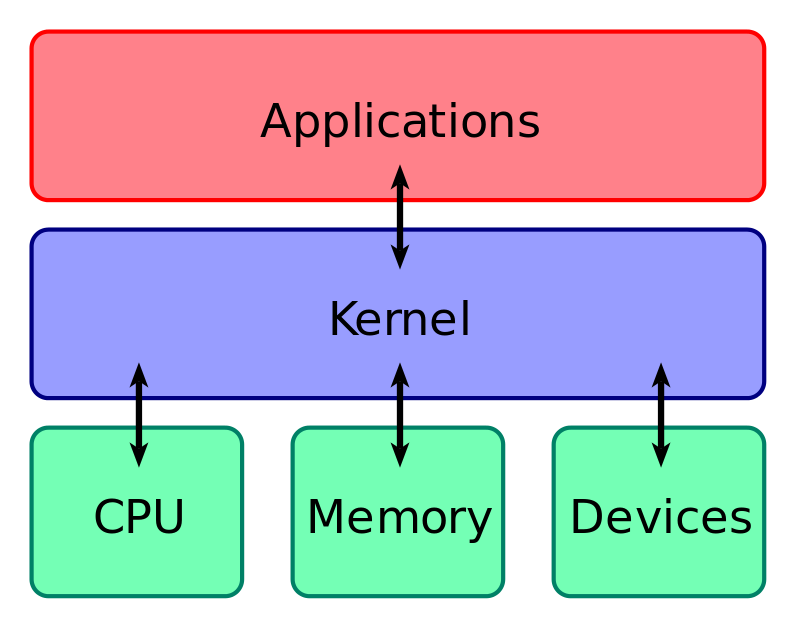
\includegraphics[width=0.75\textwidth]{Figures/Kernel_Layout.png}}
\caption{Kernel connect}
\label{kernel}
\end{figure}

\lstinputlisting[caption=contoh dasar kode program kerne membuat hello world,label={lst:kode dasar}]{src/contoh.tex}

\subsection{struktur data kernel}
	Ketika kernel melakukan sebuah proses, data-data proses tersebut akan disimpan secara periodik ke dalam bentuk file-file. Untuk dapat melihat data kernel, maka file-file tersebut harus diparsing setiap saat dikarenakan datanya yang dinamis \cite{raharja2001pengenalan}. Cara termudah untuk melakukan hal tersebut yaitu menggunakan perintah \textbf{cat} \ref{lst:kode dasar2}

\lstinputlisting[caption=Perintah cat pada linux,label={lst:kode dasar2}]{src/cat.sh}
File-file ini akan tersimpan di dalam direktori yang tersetruktur dalam direktori /proc.

\subsection{Instalasi}
Setelah kita memahami tentang kernel dan juga struktur data kernel, selanjutnya kita akan mencoba install kernel sebelum itu kita dapat cek versi kernel kita dengan mengetikan pada terminal 
\begin{verbatim}
$ uname -r 
\end{verbatim}
\textbf{uname} ini merupakan perintah untuk mengetahui sistem informasi dan \textbf{-r} merupakan perintah untuk menampilkan versi kernel.
 
Untuk instalasi sendiri terdapat beberapa cara yaitu kamu bisa mendownload package dan mencompile dari sumber atau bisa juga hasil download package management tools.
dengan mengetikan pada terminal
\begin{verbatim}
$ sudo apt install linux-generic-lts-vivid
\end{verbatim}
 sebagai contoh : \textbf{sudo apt install 3.19.0-43-generic} setelah itu tinggal reboot maka kernel yang kita compile tadi akan terinstall.
cara alternatif selain itu kita dapat langsung meng-\textit{upgrade} versi kernel dengan menggunakan \textbf{dist-upgrade} maka itu akan mengupdate semua package di dalam sistem. 
 \begin{verbatim}
$ sudo apt dist-upgrade
\end{verbatim}

Setelah melakukan penginstalan sebuah kernel, maka itu akan menambah beberapa file system yang ditambahkan di direktori /boot
kamu akan mendapatkan beberapa file untuk versi kernel yang berbeda seperti :
\begin{enumerate}
\item \textbf{vmlinuz} - ini adalah kernel linux yang sebenarnya
\item \textbf{initrd} - ini digunakan sebagai sistem berkas sementara sebelum memuat kernel
\item \textbf{system.map} - ini sebagai table simbol 
\item \textbf{config} - ini sebagai pengaturan kernel, jika kamu mencompile kernel sendiri maka kamu dapat mengatur modul-modul yang dimuat
\end{enumerate}
Ketika direktori /boot kehabisan ruang penyimpanan, kamu dapat menghapus versi lama dari file-file atau package yang lama. Tapi harus berhati-hati ketika melakukan pemeliharaan di dalam direktori ini karena ditakutkan akan menghapus kernel yang digunakan secara tidak sengaja.

\subsection{Komponen Kernel}
Dalam cabang kernel \textbf{/usr/src/linux}, komponen kernel disimpan didalam berbagai subdirektori yaitu :
 \begin{table}[h]
		\caption{Komponen Kernel}
		\label{Komponen kernel}
			\begin{tabular}{|c|l|}
			\hline
			Subdirektori&Keterangan\\
			\hline
			./drivers& Berisi kode untuk jenis hardware pendukung\\
			\hline
			./fs& Berisi kode filesystem pendukung\\
			\hline
			./net& Berisi kode jaringan pendukung\\
			\hline
		\end{tabular}
		\end{table}

\subsection{Shell}
\subsubsection{Pengertian}
Shell menyediakan sebuah antarmuka untuk sistem unix, untuk mengumpulkan masukan yang diinputkan dan menjalankan program berdasarkan apa yang kita input. Ketika program dieksekusi , maka akan menampilkan \textit{output} sebuah program. 
jadi, shell ini dapat kita artikan sebagai sebuah lingkungan dimana kita dapat menjalankan perintah, program, dan \textit{shell scripts}.
shell menetapkan sendiri perintah dan fungsi sebagai berikut :
\begin{enumerate}
\item \textbf{Shell Prompt}
prompt,\$, atau yang biasa kita sebut \textit{command prompt}, Shell ini membaca \textit{inputan} kalian setelah anda tekan \textbf{Enter}, lalu perintah tersebut akan dieksekusi dengan melihat kata pertama dari inputan kalian.
Contoh sederhana dari \textit{\textbf{date} command}, yang mana akan menampilkan tanggal dan waktu sebagai berikut :
\begin{verbatim}
$date
\end{verbatim}

\item{Shell Types}
terdapat 2 tipe shells yaitu :
\begin{itemize}
\item Bourne shell, Jika kalian menggunakan Bourne-type shell, karakter \$ merupakan default prompt 
Bourne shell memiliki sub kategori sebagai berikut :
\subitem Bourne shell (sh)
\subitem Korn shell (ksh)
\subitem Bourne Again Shell (bash)
\subitem Posix shell (sh)
\item C shell, jika kalian menggunakan C-type shell, karakter \% merupakan default prompt
 sedangkan C shell memiliki sub kategori 
\subitem c shell (csh)
\subitem Tenex/TOPS C shell (tcsh)
\end{itemize}

\item{shell script}
konsep dasar dari shell script selalu diawali dengan tanda \# yang menggambarkan langkah-langkah
Contoh script 
kita asumsikan membuat sebuah test.sh seperti berikut :
\begin{verbatim}
#!/bin/sh
\end{verbatim}
perintah tersebut biasa disebut shebang, yang mana simbol \# disebut hash dan ! disebut bang.
Untuk membuat script yang terdapat perintah ini, kalian harus menetapkan \textit{shebang} di baris pertama dan selanjutnya diikuti dengan perintah tambahan seperti berikut
\begin{verbatim}
#!/bin/bash
pwd
ls
\end{verbatim}
\end{enumerate}

\subsubsection{Pipeline}
Pipeline (|) merupakan fasilitas di shell UNIX yang berfungsi untuk memberikan input dari suatu proses dari output proses
yang lain. Misalkan sebagai contoh :
sebelum menggunakan pipeline
\begin{verbatim}
askahar@pc:~$ find *
contoh
test
\end{verbatim}

menggunakan pipeline :
\begin{verbatim}
askahar@pc:~$ find * | grep test
test
askahar@pc:~$
\end{verbatim}
Jadi, jika kita tarik kesimpulan dari perintah diatas bahwa output dari perintah find menjadi input dari perintah grep yang kemudian hanya mengambil kata \"test\" dari output find.


\subsection{Commands and Utilities}
Terdapat berbagai perintah dan utilitas yang kalian dapat gunakan, ada lebih dari 250 perintah standar plus dengan yang disediakan melalui \textit{software} dari pihak ke-3. 

Beberapa perintah yang biasa digunakan sebagai berikut pada tabel \ref{commands}:

\begin{table}[h]
		\caption{Perintah dasar Unix}
		\label{commands}
			\begin{tabular}{|c|l|}
			\hline
			\textbf{Perintah}& \textbf{Keterangan} \\
			\hline
			cat&Perintah yang digunakan untuk membaca, memodifikasi atau concatenate file teks\\
			\hline
			cd&Perintah untuk mengubah direktori saat ini dan berpindah ke direktori yang ditentukan\\
			\hline
			chmod&Perintah untuk mengubah ijin dari satu atau lebih file\\
			\hline
			cp&Perintah untuk mencopy files dan direktori\\
			\hline
			df&Perintah untuk menampilkan jumlah ruang penyimpanan yang tersedia pada sistem file yang mengandung argumen setiap nama file\\
			\hline
			env&Perintah ini untuk menjalankan program environment yang dimodifikasi\\
			\hline
			ifconfig&Perintah ini digunakan untuk mengkonfigurasi antarmuka jaringan kernel,hal ini biasanya hanya digunakan ketika debugging atau sistem tuning\\
			\hline
			ifup&Perintah ini digunakan admin untuk mengkonfigurasi antarmuka jaringan dan mengaktifkan koneksi jaringan\\
			\hline
			ifdown&Perintah ini digunakan untuk menutup antarmuka jaringan dan menonaktifkan koneksi jaringan\\
			\hline
			iptables&Perintah yang memungkinkan atau blok lalu-lintas pada linux host dan dapat mencegah aplikasi tertentu dari menerima atau mengirimkan permintaan\\ 
			\hline
			kill&Perintah ini digunakan mematikan proses atau aplikasi dengan aman\\
			\hline
			ls&Perintah untuk menampilkan daftar file dan direktori\\
			\hline
			mkdir&Perintah ini digunakan untuk membuat direktori baru dengan nama path\\
			\hline
			netconfig/netcfg&Perintah ini digunakan untuk menkonfigurasi jaringan, mengaktifkan produk-produk jaringan dan menampilkan informasi konfigurasi jaringan\\
			\hline
			netstat&Perintah ini digunakan untuk menyediakan informasi dan statistik tentang protokol dalam penggunaan dan koneksi jaringan TCP/IP,untuk mengetahui proses dan program yang aktif pada komputer dan yang terdapat dalam satu jaringan\\
			\hline
			 nslookup&Perintah ini digunakan untuk dapat memasukkan nama dan menemukan IP sesuai dengan nslookup, berguna untuk membantu menemukan nama host\\
			\hline
			passwd&Perintah ini digunakan untuk memperbarui sandi pengguna saat ini\\
			\hline
			ping&Perintah ini digunakan untuk memverifikasi alamat IP tertentu dan dapat menerima permintaan IP, selain itu digunakan untuk menguji konektivitas dan menentukan waktu respon serta memastikan pengguna bahwa host bekerja\\
			\hline
			ps&Perintah ini digunakan untuk melaporkan status proses saat ini dalam sistem\\
			\hline
			pwd&Perintah ini digunakan untuk menampilkan nama direktori yang sedang dijalankan saat ini\\
			\hline
			sudo&Perintah ini digunakan untuk memungkinkan administrasi sistem yang memberikan user kemampuan untuk menjalankan beberapa aatau semua perintah dan argument\\
			\hline
			ssh&Perintah ini digunakan untuk mengakses remote komputer yang aman dan digunakan admin meremote kontrol server\\
			\hline
			uname&Perintah ini digunakan untuk menampilkan nama sistem operasi saat ini dan dapat mencetak inforamsi sistem\\
			\hline
			vi&Perintah ini digunakan sebagai teks editor yang memungkinkan pengguna untuk mengontrol sistem dengan hanya keyboard, mouse dan penekanan tombol \\
			\hline
			vmstat&Perintah ini digunakan untuk menampilkan sistem dan laporan informasi tentang berbagai proses, memori, paging dan aktivitas CPU. selain itu metode ini digunakan untuk menentukan mana masalah perlambatan dapat terjadi dalam sistem\\
			\hline
			wget&Perintah ini digunakan untuk utilitas jaringan dalam mengambil file web yang mendukung HTTP, HTTPS dan protokol FTP\\
			\hline
		\end{tabular}
		\end{table}

\subsection{Struktur direktori Linux}
Pada direktori root linux terdapat beberapa direktori standar yang biasa ada pada banyak distro linux, direktori tersebut sebagai berikut pada tabel \ref{direktori} :
\begin{table}[h]
		\caption{Direktori Linux}
		\label{direktori}
			\begin{tabular}{|c|l|}
			\hline
			\textbf{Direktori}& \textbf{Isi} \\
			\hline
			/bin&Berisi file-file binary standar yang dapat digunakan oleh seluruh user \\
			\hline
			/boot&Berisi file-file yang digunakan untuk booting Linux termasuk kernel image\\
			\hline
			/dev& Berisi file system khusus yang merupakan refleksi device hardware yang dikenali dan digunakan sistem \\
			\hline
			/etc&Berisi file-file konfigurasi sistem, biasanya hanya boleh diubah oleh super user\\
			\hline
			/home&Berisi direktori-direktori yang merupakan direktori home untuk user biasa dan aplikasi tertentu\\
			\hline
			/lib&Berisi file-file library yang digunakan untuk mendukung kerja kernel Linux\\
			\hline
			/mnt&Direktori khusus yang disediakan untuk mounting (mengaitkan) device disk storage ke sistem dalam bentuk direktori \\
			\hline
			/prod&Berisi file system khusus yang menunjukkan data-data kernel setiap saat\\
			\hline
			/root&Direktori home untuk user root (user khusus dengan priviledges hampir tak terbatas)\\
			\hline
			/sbin&Sama halnya dengan direktori bin, tetapi hanya super user yang sebaiknya menggunakan binary-binary tersebut mengingat fungsi-fungsi binary yang terdapat di direktori ini untuk maintenance sistem\\
			\hline
			/tmp&Berisi file-file sementara yang dibutuhkan sebuah aplikasi yang sedang berjalan\\
			\hline
			/usr&Berisi library, binary, dokumentasi dan file lainnya hasil instalasi user\\
			\hline
			/var&Berisi file-file log, mailbox dan data-data aplikasi\\
			\hline
		\end{tabular}
		\end{table}

\section{System Startup}
Untuk menyesuaikan proses booting melibatkan bagaimana kita memahami tentang script startup. Masalah umum yang muncul diberbagai titik selama proses booting serta beberapa teknik \textit{recovery}. Berfokus pada awal disk ram pada tahap proses booting, memungkinkan untuk dapat membuat keputusan sebagai disk ram yang baru dibuat.
\subsection{Menyesuaikan Proses Boot}
\begin{enumerate}
\item Overview of init
Untuk mencegah proses dijalankan pengguna dari campur dengan kernel dua wilayah yang berbeda memori untuk didefinisikan. Hal ini disebut sebagai \" kernel space memory\" dan \"user space memory\". Proses init merupakan program pertama untuk menjalankan dalam \textit{user space memory}.
 init merupakan the parent dari semua proses, perintah untuk memanggil konfigurasi init yaitu 
\begin{verbatim}
$ /etc/initlab
\end{verbatim}
\item RunLevels
Runlevels menentukan proses yang harus dijalankan secara bersama-sama.  semua proses yang dapat mulai atau berhenti di runlevel diberikan kendali oleh script \textbf{init script} atau \textbf{rc script} di dalam direktori /etc/rc.d/init.d
\end{enumerate}

\subsection{System Recovery}
Ketika sistem crash dan gagal untuk merestart diperlukan untuk mengubah proses boot normal, Bagian ini menjelaskan beberapa solusi yang sesuai untuk masalah-masalah yang dapat terjadi pada tahap berikutnya dari proses boot pada tabel \ref{recovery}
\begin{table}[h]
		\caption{System recovery}
		\label{recovery}
			\begin{tabular}{|c|l|l|}
			\hline
			\textbf{Booting Stage}&\textbf{Tipe Error}&\textbf{Solusi yang disarankan}\\
			\hline
			INIT&Corrupt root filesystem atau a faulty /etc/fstab entry&menggunakan root login prompt\\
				&kernel module fails to load atau an RC Script fails&override INIT atau menggunakan alternative runlevel\\
			\hline
			KERNEL&kernel panic& 	\\
				&hardware initialisation errors&melewati parameter bootloader parameter misalnya acpi=off\\
			\hline
			BOOT LOADER&Not installed or broken&menggunakan rescue disk atau boot disk\\
			\hline
\end{tabular}
\end{table}

\subsection{Overriding the INIT stage}
Hal ini diperlukan ketika proses boot gagal karena script init rusak, Setelah kernel ini berhasil menempatkan root filesystem ini akan mencoba untuk menjalankan /sbin/init. Tapi kerenl dapat diinstruksikan untuk menjalankan shell yang memungkinkan untuk memliki akases ke sistem sebelum services dimulai.
pada LILO atau GRUB boot prompt tambahkan parameter ini pada kernel :
\begin{verbatim}
init=/bin/bash
\end{verbatim}
Pada tahap akhir boot kernel kita harus ke bash prompt. Read-write akses ke root filesystem dengan perintah berikut :
\begin{verbatim}
mount /proc
mount -o remount, rw /
\end{verbatim}



\chapter[Sistem Keamanan Linux]
{Sistem Keamanan Linux}
\section{Sistem Keamanan Linux}
\subsection{SELinux}
	SELinux \textit{(Security Enhaced Linux)} yang mana merupakan salah satu peningkatan keamanan dari sebuah sistem operasi berbasiskan linux, keamanan yang dimaksud disini yaitu untuk membedakan antara user root dan juga user yang sifatnya terbatas atau memiliki hak akses masing-masing. Aplikasi mendasar dari SELinux ini adalah layanan FTP \textit{(File Transfer Protocol)} dan HTTP \textit{(Hyper Text Transfer Protocol)}.
SELinux ini memiliki 3 mode yaitu :
\begin{enumerate}
\item Enforcing, merupakan pengaturan keamanan yang paling ketat
\item Permissive, merupakan pengaturan keamanan yang longgar
\item Disabled, merupakan pengaturan untuk memayikan SELinux
\end{enumerate}

pada linux terdapat SELinux, di windows pun sebenarnya ada yang seperti itu namun dengan nama yang berbeda yaitu \textit{User Account Control} atau UAC berfungsi untuk menjalankan aplikasi atau membuat, mengedit dan menghapus program yang penting.


\chapter[Starvation]
{OS\\ Starvation}
\section{Starvation}
Perkembangan sistem komputer mendatang adalah menuju ke sistem multi-processing, multiprogramming, terdistribusi dan paralel yang mengharuskan adanya proses-proses yang berjalan bersama dalam waktu yang bersamaan. Hal demikian merupakan masalah yang perlu perhatian dari perancang sistem operasi. Kondisi dimana pada saat yang bersamaan terdapat lebih dari satu proses disebut dengan kongkurensi (proses-proses yang kongkuren). Dan dalam kongruensi ini pasti ada masalah yang salah satunya adalah STARVATION.

\chapter[DeadLock]
{OS\\ deadlock}
%Nama Kelompok: Sistem_Operasi_Deadlock
%Kelas: D4 TI 1B
%Alit Fajar Kurniawan(1174057) 
%Muhammad Iqbal Panggabean(1174063)
%Muhammad Afra Faris(1174041)
%Khadijah Hasanah Puteri Harahap(1174044)

\section {DEADLOCK}

\subsection {Deadlock}
\subsubsection {Pengertian Deadlock}
	Pada kesempatan ini saya akan menjelaskan tentang definisi Deadlock, Deadlock ialah suatu keadaan yang dimana dua proses atau lebih, saling menunggu proses untuk dapat melepaskan sumber daya yang sedang dijalankan. Misalnya proses A yang memperlukan suatu sumber daya, tetapi sumber saya tersebut sedang digunkana oleh proses lain. Untuk lebih paham mengenai pengertian dari deadlock dan bagaimana cara mengatasinya, anda dapat membandingkannya dengan situasi yang satu ini. Pertama, Dalam kehidupan kita tentu membutuhkan suatu pekerjaan, dan untuk memperoleh suatu pekerjaan, anda harus memiliki pengalaman yang baik, untuk dapat memiliki pengalaman yang baik anda harus bekerja.

	\begin{figure}[ht]
	\centerline{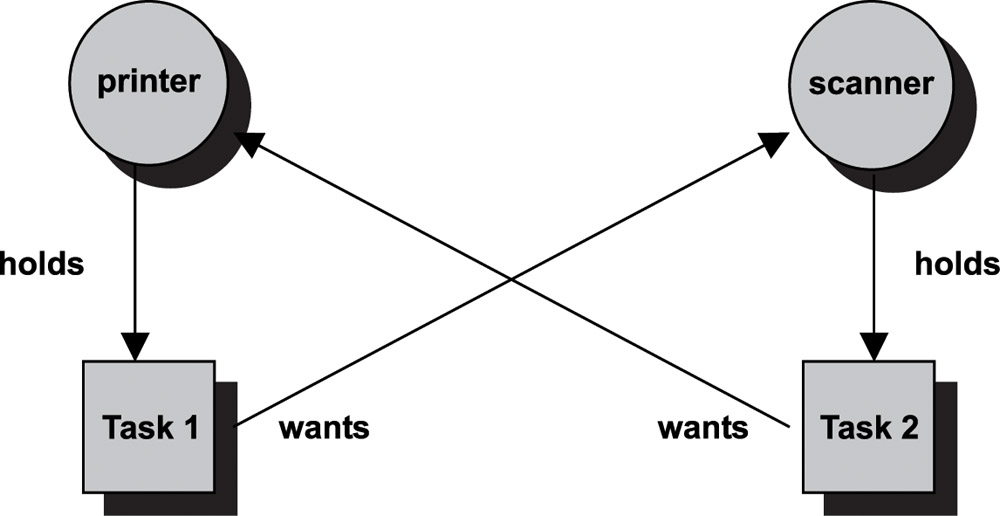
\includegraphics[width=1\textwidth]{figures/deadlock1.jpg}}
	\caption{Gambar Deadlock}
	\label{Gambar}
	\end{figure}
      
      Gambar \ref{Gambar} Contoh gambar pada saat terjadinya deadlock.

\subsection {Masalah Deadlock dan Metode Penanganan Deadlock}
\subsubsection {Masalah Deadlock}
	Deadlock merupakan dampak pengaruh dari sinkronisasi, yaitu dimana satu variabel yang digunakan oleh dua proses yang berbeda. Deadlock selalu tidak terlepas dari yang namanya sumber daya, karena hampir secara keseluruhan merupakan masalah mengenai sebuah sumber daya yang digunakan secara bersamaan. Sebuah Kelompok Proses yang diblok atau diblokir, dimana setiap proses memegang sebuah resource dan kemudian menunggu resource lain dari proses yang berada didalam proses yang sedang diBlok tersebut, biasanya dari semua proses-proses atau resource yang non preemptive..
	
\subsubsection {Metode Penanganan}
	Ada tiga Metode penanganan Deadlock:
	Yang Pertama yaitu, anda harus menggunakan satu protokol yang dapat membuat anda yakin bahwa sistem tersebut tidak akan pernah mengalami kejadian deadlock. Metode ini bisa disebut dengan Deadlock Prevention atau Avoidance.
	
	Yang Kedua, anda harus memberikan izin sistem untuk mengalami kejadian deadlock, namun setelah terjadinya deadlock anda harus dengan cepat segera untuk memperbaiki sistem yang mengalami deadlock tersebut. Metode ini biasanya disebut dengan Deadlock detection and recovery.
	
	Dan yang terakhir, anda hanya mengabaikan semua permasalahan yang terjadi secara bersamaan, dan kemudian menganggap bahwa deadlock tidak akan terjadi, metode ini digunakan dalam berbagai sistem operasi komputer, termasuk windows dan unix.

\begin{table}[H]
\begin{tabular}{|c|c|c|}
\hline
Proses & Jumlah Sumber Daya Digenggam & Maksimum Sumber Daya Dibutuhkan\\
\hline
X   & 2 & 10\\
\hline
Y   & 1 & 3\\
\hline
Z   & 3 & 7\\
\hline
Tersedia 4  &  &\\
\hline
\end{tabular}
\end{table}

\begin{table}[h]
\caption{Kondisi yang menyebabkan Deadlock}
\begin{tabular}{|c|c|}
\hline
Mutual exclusion&Hanya ada satu proses yang boleh memakai sumber daya, dan proses lain yang ingin memakai sumber daya tersebut harus menunggu hingga sumber daya tadi dilepaskan atau tidak ada proses yang memakai sumber daya tersebut.\\
\hline
Hold and wait&Proses yang sedang memakai sumber daya boleh meminta sumber daya lagi maksudnya menunggu hingga benar-benar sumber daya yang diminta tidak dipakai oleh proses lain, hal ini dapat menyebabkan kelaparan sumber daya sebab dapat saja sebuah proses tidak mendapat sumber daya dalam waktu yang lama.\\
\hline
No preemption&Sumber daya yang ada pada sebuah proses tidak boleh diambil begitu saja oleh proses lainnya. Untuk mendapatkan sumber daya tersebut, maka harus dilepaskan terlebih dahulu oleh proses yang memegangnya, selain itu seluruh proses menunggu dan mempersilahkan hanya proses yang memiliki sumber daya yang boleh berjalan. \\
\hline
Circular wait&Kondisi seperti rantai, yaitu sebuah proses membutuhkan sumber daya yang dipegang proses berikutnya.\\
\hline
\end{tabular}
\label{deadlock}
\end{table}

\subsection {Deadlock Detection}
\begin {enumerate}
\item
1. Pendeteksian secara Algoritma, yaitu dengan cara kita mengetahui jika terjadinya deadlock, deadlock terjadi jika suatu permintaan tidak dapat ditangani segera.
	
\item
2. Recovery atau Pemulihan, yaitu yang pertama menggagalkan semua proses deadlock, yang kedua mem backup semua proses yang deadlock dan kemudian silahkan melakukan restart di semua proses yang sedang terjadi, yang ketiga menggagalkan semua proses yang deadlock secara berurutan sehingga tidak akan terjadi lagi deadock, dan yang terakhir yaitu menggagalkan pengalokasian resource secara berurutan hingga tidak ada deadlock.

\end {enumerate}

\subsection {Beberapa hal yang terjadi ketika mendeteksi adanya deadlock}
\begin {enumerate}
\item
1. Permintaan sumber daya dikabulkan selama memungkinkan.
\item
2. Sistem operasi melakukan scanning apakah ada kondisi circular wait secara peiodik.
\item
3. Pemeriksaan dilakukan setiap ada sumber daya yang hendak digunakan.
\item
4. memeriksa dengan algoritma tertentu.
\end {enumerate}

\subsection {Beberapa jalan untuk kembali dari deadlock}
\begin {enumerate}
\item
1. Lewat Preemption, yaitu dengan jauhkan sumber daya dari pemakainya untuk sementara waktu, tujuannya untuk memberikannya pada proses lain. strategi dengan memberikannya kesempatan pada proses lain dengan tanpa diketahui oleh pemilik dari sumber daya itu dan tergantung juga dari sifat sumber daya itu sendiri.
\item
2. Lewat melacak kembali, setelah melakukan prosesn dari preemption tersebut maka secara otomatis proses utama yang diambil sumber dayanya akan stop dan tidak akan melanjutkan prosesnya, oleh karena itu dibutuhkan langkah untuk dapat kembali pada keadaan aman, tetapi untuk menentukan keadaan aman tersebut sangatlah susah.
\item
3. Mematikan proses yang menyebabkan deadlock, ini merupakan cara yang sangat umum digunakan yaitu dengan cara mematikan semua proses yang mengalami deadlock.
\item
4. Menghindari deadlock, pada sistem permintaan untuk sumberdaya biasanya hanya dilakukan sekali saja, sistem harus sudah dapat mengenali bahwa sistem itu aman atau tidak.
\end {enumerate}

\cite{siahaan2015penyelarasan}
\cite{fauzi2013perangkat}
\cite{silberschatz2014operating}


\chapter[Baudrate]
{OS\\ Baud Rate}
%Nama Kelompok: Sistem_Operasi_BaudRate
%Kelas: D4 TI 1B
%Anggota : 
%Kevin Natanael Nainggolan(1174059) 
%Luthfi Muhammad Nabil(1174035)
%Salwaa Tania(1174047)
%Surya Pandu Prananda(1174036)

\section{Baud Rate}

\subsection {Pengertian Baud Rate}
	Baud rate merupakan jumlah terjadi nya suatu perubahan status antara status nol dan status satu dalam waktu satu detik . Contoh nya ialah , suatu saluran memiliki sebuah baud rate 1000 , itu berarti saluran itu mampu mengirimkan setiap detik terjadi 1000 kali perubahan status  .
	
\subsection{Konsep Baud Rate}
Komunikasi secara berturut-turut sudah tidak asing lagi di era teknologi ini, salah satunya dikarenakan jumlah penghantar yang digunakan bisa lebih efektif daripada melakukannya secara sejajar. Mengapa demikian? Karena kata Berturut-turut berarti mengirim satu bit data dan selanjutnya yang diikuti oleh bit-bit data yang lain pada jalur yang sama. Karena itulah kita dapat meringkas penggunaan kabel. Dikarenakan jalur yang dilalui bersamaan, maka kecepatan komunikasi berturut-turut tidak secepat kecepatan komunikasi sejajar. Komunikasi sejajar, dapat mengirim data secara bersamaan melalui beberapa jalur. Namun, untuk proses secara keseluruhan, sistem komunikasi berturut-turut memenuhi berbagai aplikasi microcontroler. Selain itu, sistem komunikasi berturut-turut sering digunakan pada modem, USB, RS-232, dan teman-temannya.Hal yang sangat penting dalam menghubungkan dua perangkat melalui komunikasi berturut-turut adalah memastikan bahwa kedua perangkat berkomunikasi dengan bentuk yang sama, terdapat beberapa parameter yang digunakan untuk membangun komunikasi secara berturut-turut, diantaranya adalah Baud Rate, paket data, parity bit, dan synchronization bit .

Baud rate mengindikasikan seberapa cepat data dikirim melalui komunikasi berturut-turut.Satuan baud rate itu bit per second atau disingkat bps, walaupun untuk kasus tertentu dalam komunikasi sejajar, nilai bps bisa berbeda dengan nilai baud rate. Dugaan saat ini kita berpusat pada komunikasi berturut-turut, dimana setiap detik menyatakan transisi satu bit keadaan. Apabila hal ini terpenuhi, maka nilai baud rate akan sama dengan nilai bit per secondnya. Bit per second ini mengartikan bahwa berapa bit data dapat ditransfer setiap detiknya. Jika kita membalikan nilai bps ini, kita dapat memperoleh keterangan berapa lama waktu yang dipakai saat mengirim 1 bit. Nilai baud rate dapat diatur dengan standar kecepatan, diantaranya 
\begin {itemize}
	\item 1.200bps,
	\item 2.400bps, 
	\item 4.800bps, 
	\item 9.600bps, 
	\item 19.200bps, 
	\item 38.400bps, 
	\item 57.600bps,
	\item 115.200bps. 
\end {itemize}	
	Kecepata yang paling umum digunakan 9.600 bps. Ini adalah nilai yang mana kecepatan komunikasi bukalah suatu hal yang kritis untuk dipertimbangkan. Seperti contoh, jika kita ingin mengetahui nilai dari sensor warna. Mendapatkan data warna dari suatu sensor tidaklah memerlukan kecepatan komunikasi yang terlalu cepat. Agar  error tidak terjadi, kita menggunakan kecepatan standar 9.600 bps.

\begin{figure}[ht]
	\centerline{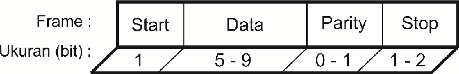
\includegraphics[width=1\textwidth]{figures/serialframe.png}}
	\caption{Serial Frame}
	\label{serialframe}
\end{figure}	
\subsection{Fungsi Baud Rate}
Baud rate dideteksi untuk mengetahui keluaran dari perangkat yang memerlukan basis serial untuk mengecek kecepatan data dan data itu sendiri. \cite{anderson1973method} Secara singkat, mendeteksi baud rate terdiri dari menentukan kecepatan transmisi dari perangkat yang mendapatkan sinyal karena perangkat penerima dapat dengan tepat mendecode sinyal dan mengkonversikannya ke perangkat. Baud rate memberitahu kecepatan data yang dapat dikirim melalui komunikasi serial. Dalam bps sendiri, berarti diketahui berapa kecepatan data yang dialirkan. Biasanya baud rate yang dipakai adalah 9600. Semakin besar baud rate yang dipakai, semakin tinggi kecepatan transfer data. Tetapi makin tinggi kecepatan maka makin beresiko mengalami error data. Untuk itu, disarankan untuk memakai baud rate standar atau dibawah 115.201.

\subsection{ Perbedaan baud rate dengan bit rate }
Kedua nya ini digunakan untuk mengukur kecepatan dalam konektivitas . Baud rate adalah ukuran berapa banyak simbol yang dikirimkan setiap sinyal . Simbol adalah setiap perubahan bentuk gelombang atau pulsa elektrik yang digunakan untuk mentransmisikan data sepanjang medium . Di sisi lain , bitrate adalah ukuran jumlah bit yang ditransmisikan . Dahulu , baud rate dan bit rate di guna kan secara bergantian karena teknik modulasi yang lebih lama dan  hanya memungkin kan satu bit untuk di masuk kan ke dalam setiap simbol . namun sekarang , setiap simbol dapat berisi lebih dari bit , sehingga bitrate menjadi jauh lebih tinggi dari

\subsection{Framing Data}
Framing data adalah teknik penyusunan data untuk dikirim melalui komunikasi serial. Pada gambar \ref{serialframe}, Data yang dikirim melalui komunikasi serial biasanya dari 5 sampai 9 bit. Pada arduino, data yang dipakai berukuran 8 bit. Urutan dari pengiriman data biasanya mengikuti endian tertentu. seperti pengiriman most-significant-bit atau least-significant-bit terlebih dahulu yang dikirim.
\subsubsection{Kit Framing Data}
Start dan Stop bit biasa dikenal sebagai synchronization bit yang biasanya berukuran 2 atau 3 bit. Bit-bit ini mengawali dan mengakhiri pengiriman data. Start bit selalu diberi ukuran 1 bit sedangkan stop bit dapat diberi 1 atau 2 bit tergantung bagaimana pengguna perangkat keras atau pengkonfigurasi perangkat keras menggunakaannya. Jika tidak memerlukan konfigurasi, nilai stop bit dapat dibiarkan menjadi sebesar 1 bit. seperti pada gambar \ref{serialframe}.
Posisi idle pada komunikasi serial bernilai 1. Start bit diidentifikasi dengan adanya transisi dari keadaan idle atau diam. yaitu dari 1 ke 0, sedangkan stop bit adalah kebalikan transisi dari keadaan idle untuk dari 0 ke 1.
Bit Parity dalam framing data bersifat opsional dan dapat diabaikan. Parity bit digunakan untuk transfer data yang dipengaruhi oleh noise. Namun penggunaan bit parity dapat memperlambat kecepatan komunikasi atau transfer. Penggunaan bit parity juga dibutuhkan sebuah sinkronisasi antara transmitter dengan receiver karena dilakukan untuk mengurangi kemungkinan kesalah dalam interpretasi data dalam perangkat keras.

\subsection{Contoh Pengiriman Data}
Dengan contoh saat kita mau mengirim kata OK. komunikasi akan memiliki 2 paket data. Kode ASCII untuk ;O' adalah 79 dalam desimal sedangkan huruf 'K' adalah 75. Data yang terkirim lebih dahulu adalah least-significant bit. Karena data dikirim dengan kecepatan 9600 bps, maka setiap bit memerlukan waktu selama 1/9600 = 104 mikrodetik/bit. Dalam arduino, setting baud rate dapat dilakukan dengan kode :
\begin{verbatim}
Serial.begin(9600);
\end{verbatim}
Kode tersebut menandakan bahwa kecepatan serial adalah 9600 bps atau 9600 bit per detik.



%\chapter[PySerial]
%{OS\\ PySerial}
%\section{Py Serial}

	\subsection{Python}
	Python adalah bahasa pemrograman yang dibuat oleh Guido van Rossum dan populer sebagai bahasa pemrograman scripting dan Web. Mengacu pada ide wikipedia, Python adalah bahasa pemrograman interpretatif multiguna dengan filosofi desain yang berfokus pada keterbacaan kode. 
	Python dikenal sebagai bahasa pemrograman yang menggabungkan nilai nilai kapabilitas, kemampuan, dengan sintaks kode yang sangat begitu jelas, dan dilengkapi dengan fungsi penyimpanan standar yang menjadikannya komprehensif dan komprehensif. 
	Python mendukung pemrograman multi-paradigma, khususnya, tetapi tidak terbatas, pada pemrograman berorientasi objek, pemrograman imperatif, dan pemrograman fungsional. 
	Python memiliki salah satu fitur yang sangat unik yaitu sebagai bahasa pemrograman dinamis yaitu yang datang dengan manajemen memori otomatis. Seperti bahasa 
	pemrograman dinamis lainnya, python umumnya digunakan sebagai bahasa scripting meskipun dalam prakteknya penggunaan bahasa ini lebih luas termasuk konteks penggunaan yang umumnya tidak dilakukan menggunakan bahasa scripting. 
	Python dapat digunakan untuk berbagai tujuan pembuatan perangkat lunak atau pun pengembangan perangkat lunak dan dapat dijalankan di berbagai platform sistem operasi. Python adalah salah satu contoh bahasa tingkat tinggi. 
	Contoh lain dari bahasa high-rise adalah pascal, c ++, perl, java, dan seterusnya. Sedangkan bahasa tingkat rendah adalah bahasa mesin atau bahasa assembly. 
	Secara sederhana. komputer hanya dapat menjalankan program yang ditulis dalam bahasa mesin. Karena itu. jika sebuah program ditulis dalam bahasa tinght yang tinggi. maka program tersebut harus diolah terlebih dahulu sebelum dapat dijalanlon di komputer. 
	Ini adalah salah satu kekurangan bahasa tingkat tinggi yang membutuhkan waktu untuk memproses suatu program sebelum dijalankan. Namun, bahasa tingkat tinggi memiliki banyak kelebihan. Bahasa tinglrat yang tinggi mudah dipelajari. mudah ditulis. mudah dibaca. dan tentu saja mudah menemukan kesalahan. Bahasa tingkat tinggi juga mudah dibawa untuk dicocokkan dengan mesin yang menjalankannya. 
	
	\subsection{Kelebihan}
		\begin{itemize}
			\item Dapat lebih cepat dalam pembuatan sistem aplikasi.
			\item Programnya lebih fleksible, singkat, dan sederhana.
			\item Dapat lebih mudah hindari pencatatan kode.
			\item Dapat lebih cepat dalam membuat sistem aplikasi dengan menggunakan objek yang telah ada.
			\item Mempunyai dukungan pemrograman dengan skala yang besar.
			\item Ekstensinya lebih sederhana juga berkas binernya kecil.
			\item Dapat memodifikasi atau merubah aplikasi tanpa menghentikannya.
			\item Kecepatan dalam mengeksekusi bertambah juga melindungi kode sumber.
		\end{itemize}
		
	\subsection{Kekurangan}
		\begin{itemize}
			\item Pyhton tidak efisien sebagai sebuah statis, berbeda dengan bahasa C yang dapat mempunyai penugasan yang lebih luas dari python.
			\item Python adalah sebuah interpreter, jadi tidak begitu baik dalam pengantar komponen performa kritis.
			\item Tidak bisa menjadi dasar bahasa pemrograman implementasi di beberapa komponen.
			\item Tidak memberikan keefensiensian yang menyeluruh.
		\end{itemize}
		
	\subsection{Komunikasi Serial}
		Langkah - langkah untuk melakuan komunikasi serial adalah sebagai berikut :
		
		\begin{enumerate}
			\item Open Phyton Shell
			
				\begin{figure}[ht]
			\centerline{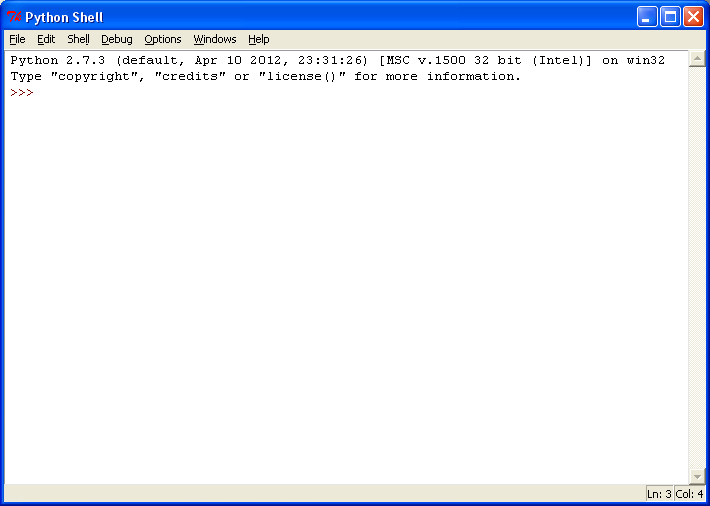
\includegraphics[width=0.5\textwidth]{figures/pyshell.png}}
			\caption{Python Shell}
			\label{pyshell}
			\end{figure}
			
			\item Buat new window seperti atau bisa juga dengan (Ctrl + N), agar muncul window baru.
				
				\begin{figure}[ht]
			\centerline{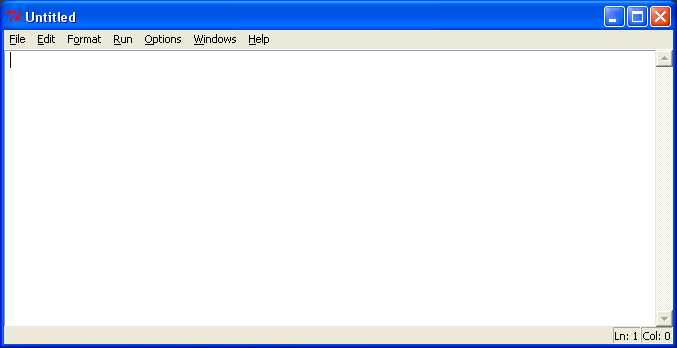
\includegraphics[width=0.5\textwidth]{figures/pyshellnew.png}}
			\caption{New Window}
			\label{pyshellnew}
			\end{figure}
			
			\item Copykan atau ketikkan script ini :
				\begin{verbatim}
					    import serial
						ser = serial.Serial(‘com10’,9600,timeout=1)
						from Tkinter import *
						root=Tk()
						def task():
						a=ser.readline(1)
						print “nilai= ” + a
						root.after(200,task)
						root.after(200,task)
						root.mainloop()
					\end{verbatim}
					
			\item Dibawah ini adalah hasilnya :
			akan muncul window:
			
			\begin{figure}[ht]
			\centerline{
\includegraphics[width=0.5\textwidth]{figures/tkser.png}}
			\caption{TK Window}
			\label{tkser}
			\end{figure}
			
			dan di Python Shell akan muncul :
			
			\begin{figure}[ht]
			\centerline{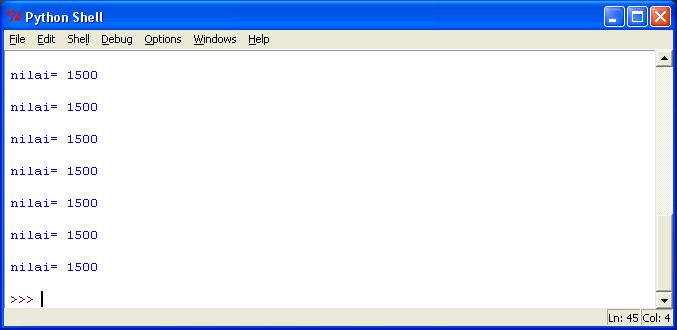
\includegraphics[width=0.5\textwidth]{figures/tkpython.png}}
			\caption{TK Window}
			\label{tkpython}
			\end{figure}
			
		\end{enumerate}
		
		Penjelasannya : 
		\begin{itemize}
			\item import serial
			bagian diatas ini mempunyai fungsi untuk melibatkan module serial sehingga dapat digunakan pada Python.
			
			\item \begin{verbatim} ser = serial.Serial(‘com10’,9600,timeout=1)\end{verbatim}
			Bagian diatas ini berfungsi sebagai pendeklerasian variabel ser sebagai serial port yang propertinya adalah konfigurasi nomer port= COM10, baudrate= 9600, dan timeout=1.
			\item \begin{verbatim} a=ser.readline() \end{verbatim}
			Bagian diatas ini berfungsi untuk membaca data dari serial lalu menampungnya pada variabel a sebagai buffer.
			\item \begin{verbatim} print “nilai= ” + a \end{verbatim} 
			Bagian diatas ini berfungsi untuk tampilkan nilai yang didapat di Python Shell. 
			\item \begin{verbatim} root.after(200,task) \end{verbatim}
			Bagia di atas ini berfungsi untuk melakukan suatu schedule setiap 200 milidetik.
			\item \begin{verbatim} root.after(200,task)	\end{verbatim}
			Bagian diatas ini berfungsi untuk mengulang suatu schedule setiap 200 milidetik.
			\item \begin{verbatim} root.mainloop() \end{verbatim}
			Bagian diatas ini berfungsi untuk melakukan perulangan atau loop.
		\end{itemize}
	
	\cite{nurjanahhack}
	\cite{rossum1995python}


\chapter[Serial Communication di Linux]
{OS\\ Serial Comm}
%kelompok 1 Sistem Operasi (Semaphore)
%Kelas D4 TI 1B
%Adam Noer Hidayatullah 1174097
%Ichsan Hizman
%Teddy
%Nisrina Aulia
%Irvan Rizkiansyah 1174043

\section{Komunikasi Serial pada Linux}
	
	\subsection{Konsep Dasar Komunikasi Serial}
	Suatu komunikasi yang dilakukan dimana suatu pengiriman data dilakukan per bit ialah dinamakan komunikasi serial, sehingga akan lebih lambat jika dibandingkan dengan komunikasi parallel seperti yang ada pada port printer yang dapat mengirim 8 bit sekaligus dalam sekali detak.
	Terdapat 2 macam cara komunikasi data serial yaitu :
		\begin{enumerate}
			\item Komunikasi data serial sinkron
			\item Komunikasi data serial asinkron
		\end{enumerate}
	
	Terdapat 2 kelompok device pada komunikasi serial yaitu :
		\begin{enumerate}
			\item Data Communication Equipment (DCE)
			Contohnya seperti scanner, printer, modem dan yang lainnya.
			\item Data Terminal Equipment (DTE)
			Contohnya sepertia terminal yang ada pada komputer.
		\end{enumerate}
	
	Keuntungan menggunakan port serial
		\begin{itemize}
			\item Masalah cable loss tidak akan menjadi suatu masalah yang besar pada komunikasi dengan kabel yang panjang, dari pada menggunakan kabel paralel. Port paralel akan mentransmisikan 0 pada tegangan 0 volt dan 1 di tegangan 1 volt, sedangkan port serial akan mentransmisikan 1 di tegangan -3 - -25 volt dan 0 di tegangan +3 - +25 volt.
			\item Hanya membutuhkan jumlah kabel yang sedikit, menggunakan 3 kabel saja pun bisa yaitu saluran Ground, saluran Transmit Data, saluran Receive Data.
			\item Populernya penggunaan mikrokontroler dan kebanyakan mikrokontroler dilengkapi dengan Serial Communication Interface (SCI) yang bisa dipaki untuk melakukan komunikasi dengan port serial pada komputer.
		\end{itemize}

	\subsection{Interprocess Communication}
	komunikasi antar proses untuk mengirim data dari satu proses ke proses yang lain, baik antar proses dalam satu komputer maupun proses dalam komputer yang berbeda
	karakteristik dari Interprocess Communincation yaitu:
		\begin{enumerate}
			\item komunikasi Synchronous dan asynchronous
				pada Sinkronisasi Synchronous, proses pengiriman dan penerimaan pada setiap pesan dan sistem ini akan berfungsi, jika sistem mengirim pesan, maka sistem hanya akan dapat merespon, sampai pesan selesai. Dalam komunikasi asynchronous, komunikasi ini dapat langsung memproses pesan, begitu pesan berada di buffer lokal, dan mengirim pesan dengan benar.
			\item Message destinations
					tempat tujuan dari sebuah pesan yang terdapat pada  sebuah computer adalah local port, yang didefinisikan berarti sebagai variable angka dengan tipe integer. Sebuah port pasti mempunyai satu penerima, akan tetapi bisa memiliki banyak pengirim.
			\item Reliability
					Keandalan suatu sistem dapat dilihat dari validitas dan integritas sistem.
					Sistem bila dilihat dari validitas, dapat dikatakan handal jika pesan yang disampaikan dijamin hingga tidak ada pesan yang hilang atau jatuh, dan sebaliknya.
			\item Ordering
				  menginginkan pesan yang terkirim dari pengirim dapat diterima sesuai dengan urutan grouping / ordering berdasarkan pesan awal yang terikirim.
		\end{enumerate}

		
	\subsection{Koneksi Linux ke Serial Port}
	Untuk melakukan setting pada suatu perangkat, terkadang harus masuk terlebuh dahulu ke dalam console box. Biasanya akan menggunakan hyperterminal, namun software bawaan seperti itu tidak terdapat pada linux pada saat linux terinstall. Maka dari itu terdapat sebuah software yang dapat digunakan pada linux untuk melakukan komunikasi serial yaitu minicom untuk menggantikan hyperterminal.
	
	Software terminal minicom dapat di install dengan mudah di linux. Pertama buka terminal pada linux lalu ketik perintah :

	sudo apt-get install minicom

	Setelah itu software akan terinstall. Kemudian koneksikan ke perangkat yang akan digunakan menggunakan kabel console pada port serial. Lalu cek pada terminal linux dengan menggunakan perintah :

	dmesg | grep tty
	
	Perintah tersebut berguna untuk mengetahui port mana saja yang digunakan, seperti pada gambar dibawah ini
	
	\begin{figure} [ht]
	\centerline{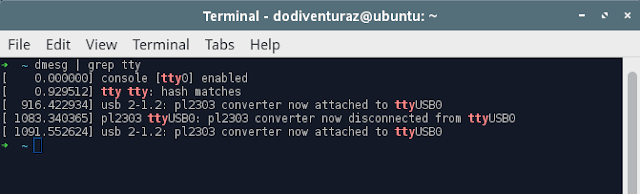
\includegraphics[width=1\textwidth]{figures/serialunix.png}}
	\caption{Gambar Status Serial}
	\label{statusserial}
	\end{figure}
	
	\ref{serialunix}
	
	Lalu ketikkan perintah :
	
	sudo minicom -s
	
	dan akan muncul seperti dibawah ini :
	
	\begin{table}[H]
		\begin{tabular}{|c|}
			\hline
			----configuration----\\
			\hline
			Filenames and paths\\
			\hline
			File transfer protocols\\
			\hline
			Serial port setup\\
			\hline
			Modem and dialing\\
			\hline
			Screen and keyboard\\
			\hline
			Save setup as dfl\\
			\hline
			Save setup as..\\
			\hline
			Exit\\
			\hline
			Exit from Minicom\\
		\end{tabular}
	\end{table}
	
	Kemudian pilih Serial Port Setup untuk mengetahui port yang terdeteksi, lalu akan muncul tampilan sebagai berikut :
	
	\begin{figure} [ht]
	\centerline{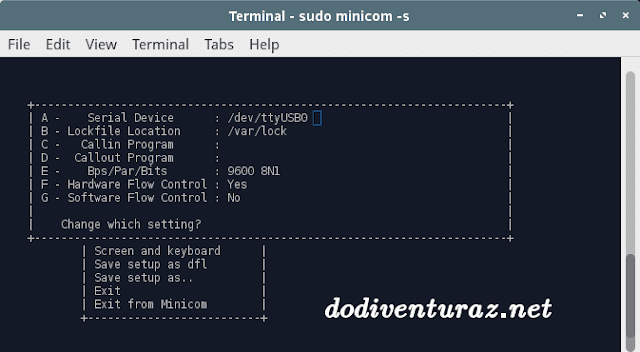
\includegraphics[width=1\textwidth]{figures/minicom.png}}
	\caption{Gambar minicom}
	\label{minicom}
	\end{figure}
	
	\ref{minicom}
	
	Lalu lakukan konfigurasi yang diperlukan sesuai kebutuhan yang diperlukan. Setelah konfigurasi selesai kembali ke menu utama dan pilih Save Setup as dfl. Kemudian pilih Exit, dan akan kembali ke terminal linux sebelumnya, kemudian ketikan perintah 
	
	minicom
	Maka Perangkat akan terkoneksi sesuai keinginan.

	




\chapter[SERIALCOMWINDOWS]
{OS\\ SERIALCOMWINDOWS}
\section{Serial Com Windows}
	\subsection{Membuka Port}
		\begin{enumerate} 
			Dokumentasi SDK Platform menyatakan bahwa ketika membuka port komunikasi, panggilan ke CreateFile memiliki persyaratan berikut:
				\item 1. fdwShareMode harus nol. Port komunikasi tidak dapat dibagikan dengan cara yang sama seperti file yang dibagikan. Aplikasi yang menggunakan TAPI dapat menggunakan fungsi TAPI untuk memfasilitasi berbagi sumber daya antar aplikasi. Untuk aplikasi yang tidak menggunakan TAPI, penanganan warisan atau duplikasi diperlukan untuk berbagi port komunikasi. Berurusan dengan duplikat berada di luar cakupan artikel ini; silakan merujuk ke dokumentasi Platform SDK untuk informasi lebih lanjut.
				\item 2. fdwCreate harus menentukan bendera OPEN_EXISTING.
				\item 3. hTemplateFile parameter harus NULL.
			Satu hal yang perlu diperhatikan tentang nama port adalah bahwa mereka secara tradisional telah COM1, COM2, COM3, atau COM4. Windows API tidak menyediakan mekanisme apa pun untuk menentukan port apa yang ada pada sistem. Beberapa sistem bahkan memiliki lebih banyak port daripada maksimum tradisional empat. Vendor perangkat keras dan pembuat perangkat serial-driver bebas memberi nama port apa pun yang mereka sukai. Untuk alasan ini, yang terbaik adalah pengguna memiliki kemampuan untuk menentukan nama port yang ingin mereka gunakan. Jika port tidak ada, kesalahan akan terjadi (ERROR_FILE_NOT_FOUND) setelah mencoba membuka port, dan pengguna harus diberitahu bahwa port tidak tersedia.
		\end{enumerate}
		\begin{enumerate}
		I / O tumpang tindih
				/ O yang tumpang tindih tidak sesederhana I / O non-tumpang tindih, tetapi memungkinkan lebih banyak fleksibilitas dan efisiensi. Sebuah port terbuka untuk operasi tumpang tindih memungkinkan beberapa utas untuk melakukan operasi I / O pada saat yang bersamaan dan melakukan pekerjaan lain ketika operasi sedang menunggu. Lebih jauh lagi, perilaku operasi yang tumpang tindih memungkinkan satu utas untuk mengeluarkan banyak permintaan yang berbeda dan bekerja di latar belakang sementara operasi masih menunggu.

				Baik dalam aplikasi single-threaded maupun multithread, beberapa sinkronisasi harus dilakukan antara mengeluarkan permintaan dan memproses hasilnya. Satu utas harus diblokir sampai hasil operasi tersedia. Keuntungannya adalah I / O yang tumpang tindih memungkinkan utas untuk melakukan beberapa pekerjaan antara waktu permintaan dan penyelesaiannya. Jika tidak ada pekerjaan yang dapat dilakukan, maka satu-satunya kasus untuk I / O yang tumpang tindih adalah memungkinkan untuk respon pengguna yang lebih baik.

		\end{enumerate}

	\begin{figure}[ht]
		\centerline{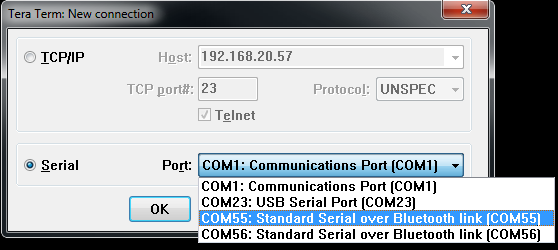
\includegraphics[width=1\textwidth]{figures/seria.png}}
		\caption{Serial Com Windows}
		\label{seria}
	\end{figure}
	Gambar \ref{seria} Contoh gambar.
		\begin{verbatim}
			HANDLE hComm;
			hComm = CreateFile( gszPort,  
                    GENERIC_READ | GENERIC_WRITE, 
                    0, 
                    0, 
                    OPEN_EXISTING,
                    FILE_FLAG_OVERLAPPED,
                    0);
			if (hComm == INVALID_HANDLE_VALUE)
				// error opening port; abort
		\end{verbatim}
	\subsection{Membaca dan menulis}
		\begin{enumerate}
			\item Membaca dari dan menulis ke port komunikasi di Windows sangat mirip dengan file input / output (I / O) di Windows. Bahkan, fungsi yang melengkapi I / O file adalah fungsi yang sama yang digunakan untuk serial I / O. I / O dapat dilakukan dengan salah satu dari dua cara: tumpang tindih atau tidak tumpang tindih. Dokumentasi SDK Platform menggunakan istilah asinkron dan sinkron untuk mengkonotasikan jenis operasi I / O ini. Artikel ini, bagaimanapun, menggunakan istilah yang tumpang tindih dan tidak terabaikan.
			\item Nonoverlapped I / O akrab bagi kebanyakan pengembang karena ini adalah bentuk tradisional I / O, di mana operasi diminta dan diasumsikan lengkap ketika fungsi kembali. Dalam kasus I / O yang tumpang tindih, sistem dapat kembali ke pemanggil segera bahkan ketika operasi tidak selesai dan akan memberi sinyal kepada pemanggil ketika operasi selesai. Program ini dapat menggunakan waktu antara permintaan I / O dan penyelesaiannya untuk melakukan beberapa pekerjaan latar belakang.
				\subsubsection{Bacaan}
					\begin{enumerate}
						\item Fungsi ReadFile menerbitkan operasi baca. ReadFileEx juga mengeluarkan operasi baca, tetapi karena tidak tersedia pada Windows 95, itu tidak tercakup dalam artikel ini. Berikut adalah potongan kode yang merinci cara mempublikasikan permintaan baca. Perhatikan bahwa fungsi memanggil fungsi untuk memproses data jika ReadFile mengembalikan TRUE. Ini adalah fungsi yang sama yang disebut jika operasi menjadi tumpang tindih. Perhatikan flag fWaitingOnRead yang didefinisikan oleh kode; ini menunjukkan apakah operasi baca tumpang tindih atau tidak. Ini digunakan untuk mencegah penciptaan operasi baca baru jika mereka luar biasa.
				
				\begin{verbatim}
				\item DWORD dwRead;
					BOOL fWaitingOnRead = FALSE;
					OVERLAPPED osReader = {0};

						// Create the overlapped event. Must be closed before exiting
						// to avoid a handle leak.
						osReader.hEvent = CreateEvent(NULL, TRUE, FALSE, NULL);

						if (osReader.hEvent == NULL)
						// Error creating overlapped event; abort.

						if (!fWaitingOnRead) {
						// Issue read operation.
						if (!ReadFile(hComm, lpBuf, READ_BUF_SIZE, &dwRead, &osReader)) {
						if (GetLastError() != ERROR_IO_PENDING)     // read not delayed?
						// Error in communications; report it.
					else
						fWaitingOnRead = TRUE;
				}
					else {    
						// read completed immediately
						HandleASuccessfulRead(lpBuf, dwRead);
			}
		}
				\end{verbatim}

				\begin{enumerate}
						\item Bagian kedua dari operasi yang tumpang tindih adalah deteksi penyelesaiannya. Pegangan acara dalam struktur OVERLAPPED diteruskan ke fungsi WaitForSingleObject, yang akan menunggu hingga objek diberi isyarat. Setelah acara ditandai, operasi selesai. Ini tidak berarti bahwa itu berhasil diselesaikan, hanya saja itu selesai. Fungsi GetOverlappedResult melaporkan hasil operasi. Jika kesalahan terjadi, GetOverlappedResult mengembalikan FALSE dan GetLastError mengembalikan kode kesalahan. Jika operasi selesai dengan sukses, GetOverlappedResult akan mengembalikan TRUE.

						
						Catatan GetOverlappedResult dapat mendeteksi penyelesaian operasi, serta mengembalikan status kegagalan operasi. GetOverlappedResult mengembalikan FALSE dan GetLastError mengembalikan ERROR_IO_INCOMPLETE ketika operasi tidak selesai. Selain itu, GetOverlappedResult dapat dibuat untuk memblokir hingga operasi selesai. Ini secara efektif mengubah operasi yang tumpang tindih menjadi operasi non-tumpang tindih dan dicapai dengan melewatkan TRUE sebagai parameter bWait.
				\end{enumerate}


			
		\end{enumerate}
			\subsubsection{Penulisan}
				\begin{enumerate}
					\item Pengarsipan data dari port komunikasi sangat mirip dengan membaca, karena menggunakan banyak API yang sama. Cuplikan kode di bawah ini menunjukkan cara menghapus dan menunggu operasi tulis selesai.
				\end{enumerate}
				\begin{verbatim}
				BOOL WriteABuffer(char * lpBuf, DWORD dwToWrite)
{
   OVERLAPPED osWrite = {0};
   DWORD dwWritten;
   DWORD dwRes;
   BOOL fRes;

   // Create this write operation's OVERLAPPED structure's hEvent.
   osWrite.hEvent = CreateEvent(NULL, TRUE, FALSE, NULL);
   if (osWrite.hEvent == NULL)
      // error creating overlapped event handle
      return FALSE;

   // Issue write.
   if (!WriteFile(hComm, lpBuf, dwToWrite, &dwWritten, &osWrite)) {
      if (GetLastError() != ERROR_IO_PENDING) { 
         // WriteFile failed, but isn't delayed. Report error and abort.
         fRes = FALSE;
      }
      else
         // Write is pending.
         dwRes = WaitForSingleObject(osWrite.hEvent, INFINITE);
         switch(dwRes)
         {
            // OVERLAPPED structure's event has been signaled. 
            case WAIT_OBJECT_0:
                 if (!GetOverlappedResult(hComm, &osWrite, &dwWritten, FALSE))
                       fRes = FALSE;
                 else
                  // Write operation completed successfully.
                  fRes = TRUE;
                 break;
            
            default:
                 // An error has occurred in WaitForSingleObject.
                 // This usually indicates a problem with the
                // OVERLAPPED structure's event handle.
                 fRes = FALSE;
                 break;
         }
      }
   }
   else
      // WriteFile completed immediately.
      fRes = TRUE;

   CloseHandle(osWrite.hEvent);
   return fRes;
}
\end{verbatim}	

\subsection{Serial Status}
	\begin{enumerate}
		\item Ada dua metode untuk mengambil status port komunikasi. Yang pertama adalah dengan mengatur event mask yang menyebabkan pemberitahuan aplikasi ketika peristiwa yang diinginkan terjadi. Fungsi SetCommMask mengatur masker kejadian ini, dan fungsi WaitCommEvent menunggu kejadian yang diinginkan terjadi. Metode kedua untuk mengambil status port komunikasi adalah secara berkala memanggil beberapa fungsi status yang berbeda. Polling, tentu saja, tidak efisien dan tidak direkomendasikan. Berikut ini contoh fungsi SetCommMask:
	\end{enumerate}
	\begin{verbatim}
	DWORD dwStoredFlags;

dwStoredFlags = EV_BREAK | EV_CTS   | EV_DSR | EV_ERR | EV_RING |\
                EV_RLSD | EV_RXCHAR | EV_RXFLAG | EV_TXEMPTY ;
if (!SetCommMask(hComm, dwStoredFlags))
   // error setting communications mask
\end{verbatim}

\cite{bai2004windows}
\cite{carvey2005tracking}
\cite{boling2003programming}			


%\chapter[usb to serial]
%{OS\\ usb to serial}
%%Nama Kelompok: Sistem_Operasi_Deadlock
%Kelas: D4 TI 1B
%Alit Fajar Kurniawan(1174057) 
%Muhammad Iqbal Panggabean(1174063)
%Muhammad Afra Faris(1174041)
%Khadijah Hasanah Puteri Harahap(1174044)

\section {USB TO SERIAL}

\subsection {Pengertian USB}
\subsubsection {Apa itu USB ?}
	Universal Serial Bus atau yang disingkat dengan USB adalah sebuah teknologi yang dapat memungkinkan para penggunanya untuk dapat menghubungkan hardware eksternal contohnya seperti printer, keyboard, harddisk, flashdisk dan perangkat keras lainnya. kecepatan trnasfer data yang didukung oleh USB sebesar 12 Mbps. pada saat ini semua PC sudah memiliki port USB sendiri minimal 2 buah port USB.

\subsection {Jenis-jenis usb}
\begin {enumerate}
\item
	USB 1.1 : Versi kabel USB 1.1 adalah versi yang pertama yang dirilis sekitar Agustus 1998 dan mulai banyak digunakan di berbagai perangkat elektronik. Versi original-nya, USB 1.0 tidak pernah digunakan pada perangkat elektronik. Versi kabel USB 1.1 ini Memiliki kecepatan up to 12 Mbps. logo yang di punyai oleh USB 1.1 ini berwarna biru dan simbol berbentuk trisula. Namun sekarang , Versi kabel USB ini sudah tidak digunakan lagi.
\item
	USB 2.0 : versi kabel USB 2.0 adalah versi yang kedua yang di rilis pada tahun 2000. Kabel usb ini memiliki kecepatan maximum up to 480Mbps dengan Hi-Speed mode atau pada Full-Speed mode memiliki kecepatan 12 Mbps . Kabel USB ini memiliki supply tegangan maximumnya ( max power out put ) adalah 2.5V, 1.8A dan akan tetap berfungsi baik jika dihubungkan dengan versi sebelumnya ( backward - compatible with USB 1.1 )
	
	Kabel USB 2.0 ini memiliki logo berwarna biru dengan tambahan tulisan HI-SPEED di atasnya dengan dasar merah. Simbol seperti trisula dengan tambahan tanda “ + ” di atasnya. Terkadang , hanya berupa sebuah trisula saja untuk menunjukkan USB yang digunakan adalah USB 2.0 , karena USB 1.1 sudah tidak digunakan lagi. Namun fungsinya kabel usb ini masih sama dengan versi sebelumnya.
\item
	USB 3.0 : Versi kabel USB 3.0 adalah versi yang ketiga yang rilis pada tahun 2008 . Kabel USB 2.0 ini memiliki kecepatan up to 5 Gbps dalam mode SuperSpeed. pada umumnya pada versi kabel USB 3.0 memiliki konektor dan soket USB berwarna biru . Maksudnya ialah sebagai tanda untuk membedakan USB 3.0 dengan versi sebelumnya .
	
	Versi kabel USB 3.0 dikenal sebagai USB Super Speed dengan gambar logo bertuliskan SUPERSPEED. Kabel USB 3.0 ini , memiliki simbol yang berbeda dengan versi kabel USB yang sebelumnya. Perbedaannya adalah ada tambahan huruf SS di pangkal trisula. USB 3.0 memiliki tampilan yang sama seperti USB 2.0 sehingga cukup kompatibel dengan USB 2.0.
	
\item
	USB 3.1 : Versi kabel USB 3.1 adalah versi yang keempat yang rilis pada tahun 2013. Kabel USB 3.1 ini memiliki kecepatan 2 kali lebih tinggi dari versi USB 3.0 yaitu 10 Gbps. Versi USB 3.1 ini juga dikenal dengan sebutan USB Super Speed + atau Super Speed USB 10 Gbps atau standar dengan Thunderbolt ( milik Apple ) . Versi USB 3.1 ini sangat kompatibel dengan USB 3.0 dan USB 2.0 . USB 3.1 ini memiliki tiga power supply tegangan , yaitu 2A pada tegangan 5V (tegangan max 10W), 5A pada tegangan 12V ( tegangan max 60W), dan 5A pada tegangan 20V ( egangan max 100W ) .
\end {enumerate}
	
\subsection {Ada Beberapa Keistimewaan dari USB}
\begin {enumerate}
\item
 PC atau komputer dapat dijadikan sebagai sebuah host
\item
 127 perangkat atu lebih dapat terhubung ke PC atau komputer dengan menggunkan hub USb secara langsung
\item
 Jika menggunakan kabel USB secara langsung hanya bisa mencapai 5 meter dan apabila menggunakan perangkat hub dapat sampai 30 meter jangkauannya
\item
 Sifat perangkat USB 'hot swappable' yang artinya apabila ada perangkat keras yang telah menggunakan port USB sifatnya plug and play
\end {enumerate}	

\subsection {Cara menghubungkan USB flash disk dengan komputer}
	USB port digunakan oleh flash disk denga tujuan untuk dapat mnghubungkan dengan komputer. fungsi dari flash disk itu sendiri yaitu untuk dapat menyimpan data dan flash disk juga memiliki batas maksimal penyimpanan. Mempelajari tentang bagaimana cara menghubungkan flash disk dengan komputer merupakan hal yang sangat mudah karena kita hanya memasukkan flash disk kedalam port USB yang tersedia di PC atau komputer. Ini merupakan salah satu cara komunikasi antara komputer atau PC dengan hardware yng dihubungkan dengan komputer atau PC dan dilakukan melalui USB To Serial.
	
	\begin{figure}[ht]
	\centerline{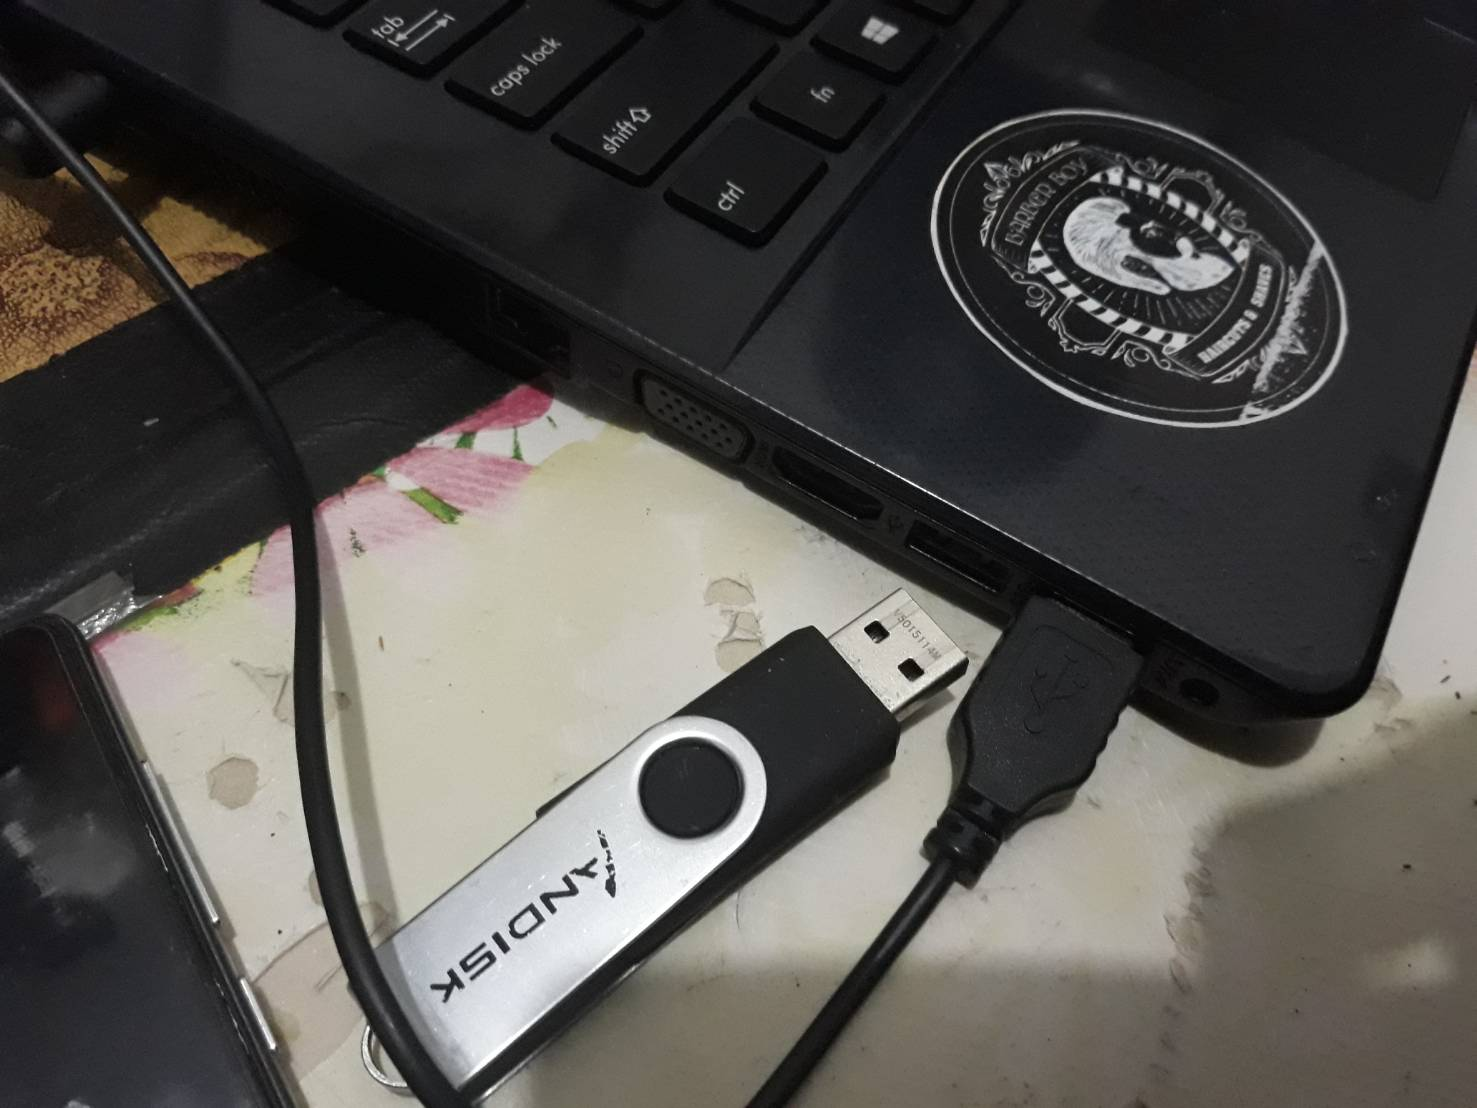
\includegraphics[width=1\textwidth]{figures/usb1.jpg}}
	\caption{Gambar memasukkan flash disk kedalam port usb pada PC}
	\label{Gambar}
	\end{figure}
      
      Gambar \ref{Gambar} Contoh gambar memasukkan flash disk kedalam port usb pada PC.
	  
\subsection {Beberapa istilah}	  
\begin{table}[H]
\begin{tabular}{|c|c|c|c|c|}
hline
No & Istilah & Arti dari Istilah\\
\hline
1   & Peripheral & Perangkat\\
2   & Hub & Sebuah alat yang digunakan untuk menghubungkan dan memperkuat sinyal dari satu PC dengan PC yang lain\\
3   & Plug and Play & Dapat langsung dikethui dan bisa digunakan oleh PC\\
4   & Port & Tempat untuk memasukkan USB\\
\hline
\end{tabular}
\end{table}


\subsection {Proses yang terjadi di USB}
	Ketika USB dimasukkan kedalam port USB pada komputer atau PC maka komputer atau PC akan mendata perangkat yang sudah tersambung ke port USB dan kemudian dilakukannya persiapan lamat memori kepada setiap perangkat yang terpasang. Proses ini disebut dengan enumerasi.
	
	
	\begin{figure}[ht]
	\centerline{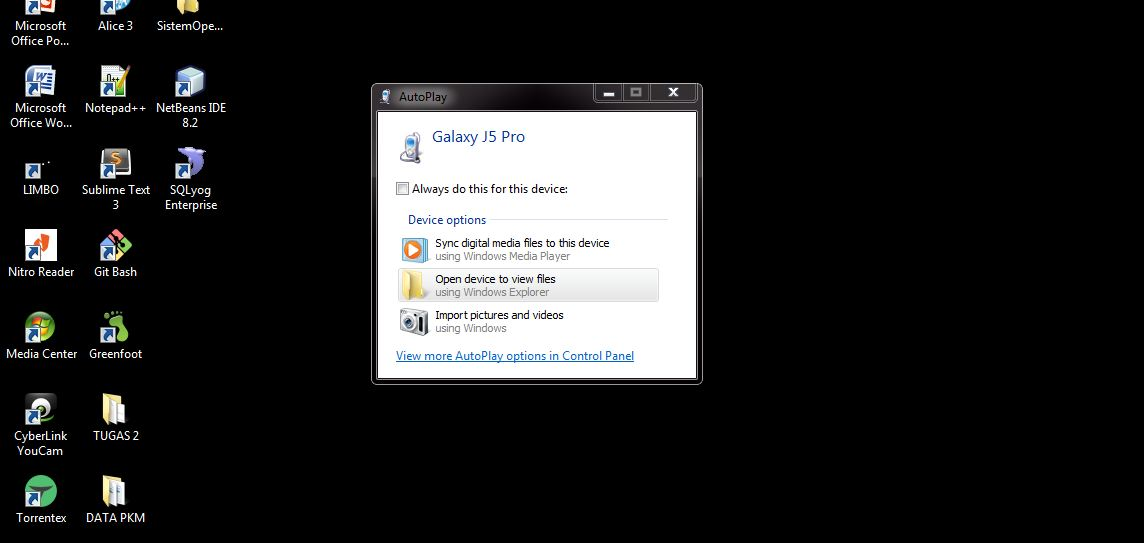
\includegraphics[width=1\textwidth]{figures/usb2.jpg}}
	\caption{Gambar proses enumerasi}
	\label{Gambar}
	\end{figure}
      
      Gambar \ref{Gambar} Contoh gambar proses enumerasi.
      
      	\cite{kulyukin2004rfid}
	\cite{turang2015pengembangan}



%\chapter[Instalasi PIP]
%{Arduino to Database\\ Instalasi PIP}
%%kelompok 1 Sistem Operasi (Proses Os)
%Kelas D4 TI 1B
%Adam Noer Hidayatullah 1174097
%Ichsan Hizman
%Teddy
%Nisrina Aulia
%Irvan Rizkiansyah 1174043

\section{PIP}

    \subsection{PIP}
	PIP adalah singkatan dari pip installs python.sebuah tool yang memudahkan programmer untuk menginstall library-library  atau disebut juga sebuah package manager untuk Python

	\subsection{cara install pip di windows}
	Sebelum melakukan peng-install-an pip, di wajibkan untuk menginstall python terlebih dahulu. Karena tanpa python tidak akan bisa mengeksekusi installer pip, dan pastikan environment variables python nya sudah ter-setting
		\begin{enumerate}
			\item download pip langsung ke website resminya di \url{<https://pip.pypa.io/en/latest/installing/>}
			\item letakan file get-pip.py ke direktori yang mudah di temukan.
			\item Buka CMD dan masuk ke direktori file get-pip.py yang tadi sudah diletakkan direktori.
			\item Pada saat di CMD langsung ketikkan python get-pip.py .
			\item tunggu proses nya hingga selesai.
			\item Setelah menginstall, kini saatnya mensetting Environment Variables supaya mudah dan dapat menjalankan pip lewat CMD tanpa harus masuk ke dalam folder hasil instalasi pip.
			\item Masuk ke dalam Control Panel - System And Security - System - advanced System Settings
			\item Lalu setelah muncul windows baru, klik pada Environment variables, terhadap sesi System variables pilih path lalu klik edit dan tambahkan
				\begin{table}[H]
					\begin{tabular}{|c|}
						\hline
						variables value ;C:/Python27/Scripts\\
					\end{tabular}
				\end{table}
				
	\subsection{Virtualenv}
	virtualenv yaitu sebuah tool yang berguna untuk mengisolasi pada lingkungan python.
	
	\subsection{lingkungan pada PIP}
	lingkungan pada PIP yaitu melingkupi binary atau executable, library, dan semua package.
	
	\subsection{kegunaan virtualenv}
			\item kegunaan virtualenv adalah untuk menginstall aplikasi atau pada lebrary python. jika tidak menggunakan virtualenv dan menggunakan user selain root,
				akan terjadi error, karena user lain pada root tidak punya akses untuk menuju ke foldedr python yang berada di system.
			\item keguaan lain virtualenv yaitu dapat membuat system pada library tetap bersih dari yang tidak dibutuhkan oleh aplikasi berbasis python lainnya.
				dengan menggunakan virtualenv kita juga dapat membuat tiap project python yang kita buat memiliki library yang berbeda beda. 
				
	\subsection {cara menginstall dan membuat virtualenv}
	cara menginstall dan membuat virtualenv:
			\item gunakan perintah "sudo pip install virtualenv" pada linux.
			\item setelah virtualenv terinstall, kita harus masuk dahulu ke dalam folder yang telah kita buat sebagai penyimpanan virtualenv.
			
	\subsection{cara mengaktifkan virtualenv}
	cara mengaktifkan virtualenv:
	buat perintah:
			\item source (namafolder)/bin/activate
				(namafolder) adalah nama folder virtualenv.
				  
	\begin{figure} [ht]
		\centerline{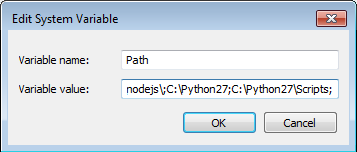
\includegraphics[width=1\textwidth]{figures/setting-env.png}}
		\caption{Gambar Setting Environment pip}
		\label{setting-env}
	\end{figure}
	
	\ref{setting-env}
	
	Harus sesuai dengan direktori hasil instalasi pip. Lalu untuk melakukan pengetesan dari berhasil atau tidak berhasilnya instalasi pip, dengan cara buka CMD lalu ketikkan perintah pip, maka akan muncul seperti gambar dibawah ini.
	
	\begin{figure} [ht]
		\centerline{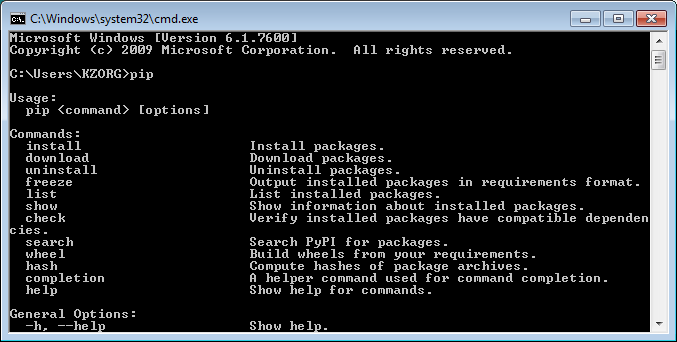
\includegraphics[width=1\textwidth]{figures/pip-terinstall.png}}
		\caption{Gambar pip yang Sudah Ter-install}
		\label{pip-terinstall}
	\end{figure}
	
	\ref{pip-terinstall}
				  
		\end{enumerate}

	\subsection{cara upgrade pip}
		\begin{item}
			\item python -m pip install -U pip
		\end{itemize}
		
	
	Dirangkum dari makalah \cite{feautrierpip}
	Dirangkum dari makalah \cite{nation2011qutip}
	Dirangkum dari artikel \cite{jewett2016moltemplate}


%\chapter[MySQL]
%{Arduino to Database\\ MySQL}
%\section{Cara Insert Database Mysql}

	\subsection{Database Mysql}}
	Basis data merupakan istilah yang mengacu kepada kumpulan data yang saling berhubungan satu sama lain, dan perangkat lunak harus mengacu pada sistem manajemen basis data DBMS. Jika konteksnya jelas, banyak administrator dan programer menggunakan istilah basis data untuk kedua makna, dan juga  merupakan sekumpulan data yang membentuk file yang saling berhubungan dengan format tertentu untuk membentuk data atau informasi baru. Atau database adalah kumpulan data yang saling berhubungan satu sama lain yang diatur berdasarkan skema atau struktur tertentu. Di komputer, basis data disimpan di perangkat penyimpanan perangkat keras, dan dengan perangkat lunak tertentu yang dimanipulasi oleh minat atau minat tertentu. 
	Hubungan atau hubungan data biasanya ditunjukkan oleh kunci dari setiap file. MySQL adalah sistem manajemen basis data perangkat lunak atau perangkat lunak SQL atau DBMS Multithread dan multi user. mysql sebenarnya merupakan turunan dari salah satu konsep utama dalam database untuk seleksi atau seleksi dan entri data yang memungkinkan operasi data dilakukan dengan mudah dan otomatis. 
	Michael Widenius merupakan seseorang yang menciptakan mysql pada tahun 1979, seorang programmer komputer swedia yang mengembangkan sistem database sederhana yang disebut unireg yang menggunakan koneksi mesin database isam tingkat rendah dengan pengindeksan. mysql adalah salah satu jenis server basis data yang paling populer.mysql menggunakan bahasa sql untuk mengakses database-nya. lisensi mysql adalah lisensi foss exception dan ada juga versi komersial. 
	Mysql tag adalah database sumber terbuka paling populer di dunia, dan sebenarnya merupakan turunan dari salah satu konsep utama dalam database yang sudah ada di sql. konsep operasi pada database terutama sql adalah untuk menseleksi atau seleksi dan entri data yang memungkinkan pengoperasian data dilakukan secara otomatis dengan mudah. 
	
	\subsection{Cara Penulisan Dasar Query INSERT}
	
	jika kita mengutip dari manual resmi MySQL sendiri, penulisan dasar perintah INSERT adalah seperti dibawah ini :
	
	\begin{verbatim}
		INSERT [LOW_PRIORITY | DELAYED | HIGH_PRIORITY] [IGNORE]
		[INTO] tbl_name [(col_name,...)]
		{VALUES | VALUE} ({expr | DEFAULT},...),(...),...
		[ ON DUPLICATE KEY UPDATE
		col_name=expr
		[, col_name=expr] ... ]
	\end{verbatim}
	
	\subsection{Cara Penggunaan Query INSERT...VALUES}
	Disini kita akan membahas perintah INSERT yang paling sederhana, yakni:
	
	\begin{verbatim}
		INSERT INTO nama_table VALUES (nilai_kolom1, nilai_kolom2,...);
	\end{verbatim}
	
	nama_table merupakan nama tabel yang akan kita input, dan nilai_kolom1 merupakan nilai yang akan kita imputkan ke dalam tabel tersebut, dan juga seterusnya untuk nilai kolom. Di nilai kolom haris berada dalam tanda kurung dan dipisah oleh tanda koma.
	
	Gambar dibawah adalah contoh memasukkan sebaris data :
	
	\begin{figure}[ht]
			\centerline{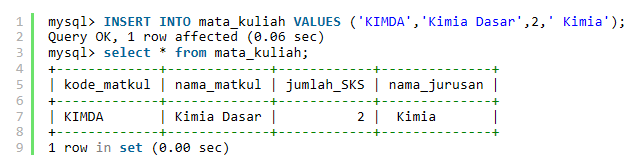
\includegraphics[width=0.5\textwidth]{figures/insert.png}}
			\caption{Insert}
			\label{insert}
			\end{figure}
			
	Kita juga bisa langsung memasukkan dua baris data ataupun lebih secara langsung hanya dengan satu perintah query INSERT, kita hanya butuh untuk memasukkan data di baris selanjutnya di belakang perintah, dengan bentuk seperti ini :
	
	\begin{verbatim}
		INSERT INTO nama_table VALUES (nilai_kolom1a, nilai_kolom2a,...), 
		(nilai_kolom1b, nilai_kolom2b,...);
	\end{verbatim}
	
	Gambar dibawah ini adalah contoh penambahan data dua baris sekaligus :
	

%\chapter[PostgreSQL]
%{Arduino to Database\\ PostgreSQL}
%\section{Cara Menghubungkan Python Dengan PostgreSQL}

\subsection{Definisi PostgreSQL}
\cite{momjian2001postgresql}PostgreSQL adalah database server dengan basis open source yang paling maju. PostgreSQL sendiri sudah dipakai oleh banyak kalangan di luar negeri karena faktor keamanan yang cukup terjamin. Seperti database server lainnya, PostgreSQL memakai bahasa pada umumnya yaitu standard SQL tetapi beberapa syntax diubah untuk kepentingan keamanan.

%\chapter[MongoDB]
%{Arduino to Database\\ MongoDBL}
%%Nama Kelompok: Sistem_Operasi_Deadlock
%Kelas: D4 TI 1B
%Alit Fajar Kurniawan(1174057) 
%Muhammad Iqbal Panggabean(1174063)
%Muhammad Afra Faris(1174041)
%Khadijah Hasanah Puteri Harahap(1174044)

\section {Insert Database MongoDB}

\subsection {MongoDB}
\subsubsection {Pengertian MongoDB}
MongoDB adalah platform lintas platform untuk sistem database yang berorientasi  dokumen. 
MongoDB diklasifikasikan sebagai database NoSQL dengan menghindari struktur basis data relasional berbasis tabel tradisional yang mendukung JSON sebagai dokumen dinamis (MongoDB menyebutnya dalam format BSON), membuatnya lebih mudah dan lebih cepat untuk mengintegrasikan beberapa data aplikasi. 
Dirilis di bawah Lisensi Publik Umum GNU Affero dan kombinasi lisensi Apache, MongoDB adalah perangkat lunak bebas dan sumber terbuka.

	\begin{figure}[ht]
	\centerline{
\includegraphics[width=1\textwidth]{figures/mongodb-1.jpg}}
	\caption{Gambar Lambang MongoDB}
	\label{Gambar}
	\end{figure}
      
      Gambar \ref{Gambar} Contoh gambar lambang MongoDB.

\subsection {Sejarah MongoDB}
Perusahaan ini dibangun pada Oktober 2007 oleh sebuah perusahaan New York City, 10gen (sekarang MongoDB Inc.) sebagai bagian dari platform yang direncanakan sebagai produk layanan.
MongoDB telah diadopsi sebagai perangkat lunak backend melalui banyak situs web dan layanan, termasuk Craigslist, eBay, Square, SourceForge, dan The New York Times. MongoDB adalah sistem basis data NoSQL yang paling populer. 
Perusahaan telah mengembangkan model pengembangan open source pada tahun 2009, dengan 10gen menawarkan dukungan komersial dan layanan lainnya.

\subsection {Bahasa MongoDB)
Database MongoDB ini tidak memakai bahasa yang biasa nya digunakan RDBMS ( SQL atau PL / SQL ) . MongoDB memakai bahasa BSON , dimana BSON adalah singkatan dari Binary JSON . Seperti JSON , BSON juga mendukung embedding dokumen dan dokumen lainnya dalam array dan array . Di dalam BSON ini , juga terdapat ekstensi yang memungkinkan untuk merepresentasi tipe data yang bukan merupakan bagian dari spec JSON . Contoh nya ialah BSON memiliki jenis tanggal dan jenis BinData. BSON dirancang untuk memiliki tiga karakteristik . Berikut adalah tiga karakteristik dari BSON : 

1. Ringan ( Lightweight ) yaitu Menjaga overhead spasial untuk minimum penting untuk format representasi data , terlebih lagi ketika digunakan melalui sebuah jaringan .

2. Dapat dilalui dengan mudah ( Traversable ) yaitu BSON di rancang untuk dapat dilalui dengan mudah . ini adalah properti penting dalam peran nya sebagai representasi data utama untuk MongoDB ini . 

3. Efisien ( Efficient ) :yaitu Encoding data untuk BSON dan decoding data dari BSON bisa dilakukan dengan sangat cepat dalam bahasa karena menggunakan jenis C data . 

	Bahasa BSON ini memiliki struktur bahasa yang hampir sama seperti bahasa JavaScript . Maka , ketika pengguna sudah terbiasa menggunakan JavaScript , tidak akan sulit baginya untuk menggunakan MongoDB ini .
	
\subsection { Tiga Element inti pada MongoDB }
Agar kita bisa mengerti kapabilitas MongoDB , kita perlu mempelajari element inti yang menyusun suatu database dalam MongoDB . Pada kenyataan nya , model penyimpanan data dalam MongoDB di organisasikan dalam sekelompok komponen yang terdiri dari tiga komponen . Berikut adalah komponen - komponen yang ada di dalam MongoDB :  

1. Database : ialah element pada top level . Pada database relasional , suatu database biasanya terdiri dari table dan views . Dalam MongoDB , suatu database ialah wadah secara fisik yang mencakup suatu struktur yang disebut collection . Setiap database memiliki sekelompok file tersendiri di dalam filesystem media penyimpanan . biasanya , satu server MongoDB terdiri atas beberapa database .

2. Collection : ialah sekelompok document MongoDB . Collection bisa dipadankan dengan table dalam RDBMS . Sejumlah collection bisa berada dalam satu database tapi harus memiliki nama yang berbeda - beda . Normalnya , collection - collection yang tergabung dalam satu database memiliki hubungan tertentu , meskipun tidak dituntut harus dibuat dengan suatu skema tertentu seperti hal nya table dalam RDBMS . 

3. Documents : ialah satuan atau unit data terkecil dalam MongoDB . Pada dasar nya tersusun atas sekelompok pasangan key - value . Tidak seperti record pada RDBMS , document memiliki skema yang dinamis , maksudnya ialah document yang berada dalam satu collection tidak harus memiliki sekelompok field yang sama . 

\subsection {Menggunakan MongoDB pada Mongolab}
Langkah - Langkahnya Sebagai berikut :

1. Login ke Account MongoLab.

2. Klik Create New
3. Tentukan penyedia layanan cloud yang ada dipilihan beserta region servernya

4. Pada menu Plan pilih tab Single Node untuk memilih kapasitas dan harga penyimpanannya mulai dari Gratis sampai Menengah.Sedangkan Replica Set Cluster untuk kapasistas dan harga penyimpanan dari Menengah sampai Kelas atas.(Pilihanku free pada tab single Node)

5. Pada Database isikan nama Databasenya. (nama databaseku akademik).

6. Klik Tombol Create New MongoDB Deployment.

7. Double klik database yang sudah di buat tadi .

8. Pada menu collections terdapat add collections untuk menambah tabel.

9. Isikan nama tabel pada dialog box yang muncul.setelah itu klik Create. (nama tabelku matkul).

10. Muncul tampilan baru dimana terdapat tombol add docummnet yang digunakan untuk mengisi data pada tabel yang sudah kita buat tadi.

11. Isikan data dimana untuk membedakan antara data dengan nama kolom tabel adalah dengan mengunakan symbol titik dua ":".
12. Setelah selesai klik save atau bisa save and go back untuk menyimpan data lalu kembali kehalaman sebelumnya.

13. Pada menu DISPLAY MODE terdapat dua pilihan yaitu list dan tabel. 

untuk tampilan tabel perlu di atur untuk tempilan tabelnya dengan menklik kata edit teble view.

14. Terdapat panduan berisi contoh mengatur tampilan tabelnya.

\subsection {kelebihan mongodb}

1. Kerangka untuk MongodDB MySQL berasal dari simplistream dan format media adalah format JSON.

2. Replikasi, data cadangan real-time adalah fitur yang sangat penting. MongoDB cocok untuk rilis berita atau blog, tetapi masih tidak cocok untuk digunakan dengan sistem informasi keuangan karena MongoDB tidak mendukung transaksi SQL.

3. Auto-curtail adalah fitur yang memuntahkan database besar dalam beberapa bagian untuk meningkatkan kinerja basis data. Sangat penting untuk menggunakan diri sendiri ketika pers memiliki database dalam jutaan baris, yang membantu membagi tirai.

4.MongoDB mencoba yang berikut: C, C ++, C #, Erlang, Haskell, Java, JavaScript, .NET (C # F #, PowerShell), Lippe, Perl, PHP, Python, Ruby, dan Scala

5.Cross-platform, dapat digunakan di Windows, Linux, OS X dan Solaris

6.CRUD Viewer (Create, Read, Work, Remove) terasa banyak cahaya

7.Map / Reduce, kami akan sangat membantu dalam melakukan operasi agregasi. Di mana semua entri dari koleksi dan outputnya juga akan menjadi koleksi. Anda dapat menggunakan MySQL untuk meminta pertanyaan oleh GROUP BY

GridFS, menggunakan spesifikasi untuk menyimpan data yang sangat besar

\subsection {Kekurangan MongoDB}
1.	Yang pertama kali kekurangan Maria DB adalah MongoDB harus diinstal pada server, dan jika Anda menggunakan PHP, Anda juga harus me-refresh server Anda. Driver mongoDB Anda dapat digunakan oleh PHP.

2.	Dan yang kedua adalah MARIA DB Ini belum didukung oleh hosting, tetapi dapat ditipu menggunakan MongoQQ (gratis hingga 16 MB gratis)

\subsection {cara instal mongodb}
	Pada dasarnya mongodb ialah basisdata yang bersifat open source yang berbasis dokumen dimana mongodb awalnya tersebut dibuat dengan menggunakan bahasa C++. Namun pada masa sekarang ini mongodb itu sendiri telah dikembangkan sejak tahun 2007. mongodb memiliki kelebihan yaitu performa yang dimiliki 4 kali lebih cepat dari pada mysql dan mongodb juga termasuk tidak sulit untuk dapat diaplikasikan.
	
\subsection {Menginstal MongoDB di windows}
\begin {enumerate}
\item
	Dalam proses ingin menginstal MogngoDB anda harus tau terlebih dahulu jenis windows PC atau laptop anda dan kemudian memeriksa PC atau Laptop tipe yang 32 bit atau yang 64 bit, kemudian anda melakukan donwload aplikasi atau instaler nya di beberapa link yang tersedia di internet. setelah melakukan download instaler nya maka coba lah untuk melakukan instalasi dengan cara mengklik kanan pada instaler tersebut dan mengklik run as administrator atau juga bisa melakukan double klik pada instaler tersebut.
\item
	Proses selanjutnya akan terbuka halaman untuk melakukan porses instalasi, pilih lah tombol install untuk melakukan instalasi. diharapkan apabila ingin menginstall MongoDB harus memperhatikan versi dari MongoDB nya, lebih baik menginstal MongoDB dengan versi terbaru, karena apabila kita menginstall MongoDB yang memiliki versi lama maka nantinya kita akan terus di perintahkan agar mengupdate untuk mendapatkan versi terbarunya.
\item
	Setelah menekan tombol install maka anda akan ditampilkan halaman yang menampilkan pilihan untuk memilih jenis pengaturan, dan sebaiknya anda memilih costum saja karena apabila anda memilih costum maka anda akan dapat menentukan sendiri lokasi instalasi MongoDB atau biasa disebut memillih secara manual lokasi instalasi. Dengan anda menentukan sendiri lokasi instalasi MongoDB maka nantinya anda akan mengetahui lokasi dan dapat memudahkan anda dalam mencari lokasi instalasi MongoDB.
\item
	Setelah menentukan lokasi instalasi MongoDB maka anda akan masuk ke halaman porses menginstall, anda hanya perlu menunggu beberapa waktu untuk proses install yang sedang berjalan. setelah proses instalasi berhasil kemudia klik finish. Dengan mengklik finish maka anda telah selesai melakukan instlasi MongoDB pada OS Windows.
\end {enumerate}


\section {Beberapa contoh codingan perintan untuk CRUD}
\subsection {Insert Data}
\begin{verbatim} 
> db.mahasiswa.insert(
{
nama:"Alit Afra Panggabean", 
ipk:3.9,
jurusan:"TI"
}
)

> db.mahasiswa.insert({nama:"Muhammad Afra Fajar"});
> db.mahasiswa.insert({nama:"Puteri Harahap",jurusan:"Logistik"});

\end{verbatim}

\subsection {Mengupdate Data}
\begin{verbatim} 
> db.mahasiswa.update({nama:"Alit"},{$set:{ipk:3.9}})
> db.mahasiswa.find({nama:"Sultan"}).pretty();
{
        "_id" : ObjectId("53130ee0999a7b243bad3b5b"),
        "ipk" : 3.9,
        "jurusan" : "TI",
        "nama" : "Alit"
}

\end{verbatim}

\subsection {Menghapus Data}
\begin{verbatim} 

 db.mahasiswa.remove({nama:"Sultan"})
 
\end{verbatim}


\cite{inproceedingsemanuel2013perbandingan}
\cite{articletunardi2014nosql}
\cite{articleahsana2016pertukaran}





%\chapter[SQLite]
%{Arduino to Database\\ SQLite}
%\section{Cara insert SQLite}
	\subsection{Definisi}
		\begin{enumerate}
			\item SQLite adalah sistem manajemen basis data relasional yang terkandung dalam pustaka pemrograman C. Tidak seperti banyak sistem manajemen basis data lainnya, SQLite bukan mesin basis data client-server. Semuanya, dicetak dalam program terakhir.
			\item SQLite adalah ACID-compliant dan mengimplementasikan sebagian besar standar SQL, menggunakan sintaks SQL dinamis dan yang tidak dapat menjamin integritas domain..
		\end{enumerate}
	\subsection{pengantar}
			\begin{enumerate}
				\item SQLite adalah sumber data relasional yang tertanam. Awalnya dirilis pada tahun 2000, itu dirancang untuk menyediakan cara yang mudah untuk aplikasi untuk mengelola data tanpa overhead yang sering dilengkapi dengan sistem manajemen basis data relasional khusus. SQLite memiliki reputasi sebagai sangat portabel, mudah digunakan, ringkas, efisien, dan andal.
			\end	
	\subsection{Sejarah}
		\begin{enumerate}
			\item D. Richard Hipp mendesain SQLite pada musim semi tahun 2000 ketika bekerja untuk General Dynamics dalam kontrak dengan Angkatan Laut Amerika Serikat. Hipp merancang perangkat lunak yang digunakan pada kapal perusak rudal, yang semula menggunakan HP-UX dengan database back-end IBM Informix. SQLite dimulai sebagai ekstensi Tcl.
			\item Tujuan desain dari SQLite adalah untuk memungkinkan program untuk beroperasi tanpa menginstal sistem manajemen basis data atau membutuhkan administrator basis data. Hipp berdasarkan sintaks dan semantik pada PostgreSQL 6.5. Pada bulan Agustus 2000, versi 1.0 dari SQLite dirilis, dengan penyimpanan berdasarkan gdbm (GNU Database Manager). SQLite 2.0 menggantikan gdbm dengan implementasi B-tree khusus, menambahkan kemampuan transaksi. SQLite 3.0, sebagian didanai oleh America Online, menambahkan internasionalisasi, pengetikan manifes, dan peningkatan besar lainnya.
			\item Pada tahun 2011 Hipp mengumumkan rencana untuk menambahkan antarmuka NoSQL (mengelola dokumen yang dinyatakan dalam JSON) ke database SQLite dan mengembangkan UnQLite, database berorientasi dokumen yang dapat disematkan. UnQLite dirilis sebagai database independen.
		\end{enumerate}
	\subsection{Desain}
		\begin{enumerate}
			\item Tidak seperti sistem manajemen basis data client-server, mesin SQLite tidak memiliki proses mandiri yang digunakan aplikasi untuk berkomunikasi. Sebaliknya, pustaka SQLite terhubung dan dengan demikian menjadi bagian integral dari program aplikasi. Menautkan dapat berupa statis atau dinamis. Program aplikasi menggunakan fungsi SQLite melalui panggilan fungsi sederhana, yang mengurangi latensi dalam akses database: panggilan fungsi dalam satu proses lebih efisien daripada komunikasi antar-proses. SQLite menyimpan seluruh basis data (definisi, tabel, indeks, dan datanya sendiri) sebagai file lintas platform tunggal pada mesin host. Ini mengimplementasikan desain sederhana ini dengan mengunci seluruh file database saat menulis. Operasi baca SQLite dapat multitasked, meskipun menulis hanya dapat dilakukan secara berurutan.
			\item Karena desainnya tanpa server, aplikasi SQLite memerlukan lebih sedikit konfigurasi daripada database client-server. SQLite disebut nol-conf karena tidak memerlukan manajemen layanan (seperti skrip startup) atau kontrol akses berdasarkan GRANT dan kata sandi. Kontrol akses ditangani dengan cara izin sistem file yang diberikan ke file database itu sendiri. Database dalam sistem client-server menggunakan hak akses file sistem yang memberikan akses ke file database hanya ke proses daemon.
			\item Implikasi lain dari desain tanpa server adalah bahwa beberapa proses mungkin tidak dapat menulis ke file database. Dalam basis data berbasis server, beberapa penulis akan terhubung ke daemon yang sama, yang mampu menangani kunci secara internal. Di sisi lain, SQLite harus bergantung pada kunci sistem file. Ini memiliki sedikit pengetahuan tentang proses lain yang mengakses database pada saat yang bersamaan. Oleh karena itu, SQLite bukan pilihan yang lebih disukai untuk penyebaran intensif. Namun, untuk pertanyaan sederhana dengan sedikit konkurensi, keuntungan kinerja SQLite dari menghindari overhead yang meneruskan datanya ke proses lain.
			\item SQLite menggunakan PostgreSQL sebagai platform referensi. Apa yang akan dilakukan PostgreSQL digunakan untuk memahami standar SQL. Salah satu ketidakberesan utama adalah bahwa, dengan pengecualian kunci primer, SQLite tidak memaksakan jenis pemeriksaan; jenis nilai bersifat dinamis dan tidak dibatasi oleh skema (meskipun skema akan memicu konversi saat menyimpan, jika konversi semacam itu berpotensi reversibel). SQLite berusaha mengikuti Aturan Postel.
		\end{enumerate}
		
		\subsection{Syntax Perintah Insert}
\begin{verbatim}

INSERT INTO nama_tabel [(kolom1, kolom2, kolom3, … kolomn)]
VALUES (nilai1, nilai2, nilai3,… nilaiN);
Kolom1, kolom2, kolom3 merupakan nama kolom yang ada didalam tabel sqlite yang akan kamu tambahkan data kedalam masing masing kolom tersebut.

INSERT INTO nama_tabel VALUES (nilai1, nilai2, nilai3,… nilaiN);
Contoh Perintah Insert Di SQLite


INSERT INTO siswa (id, nama, umur, alamat)
VALUES (1, 'Firdan Ardiansyah',27,'JL. KH. Atim II');
INSERT INTO siswa (id, nama, umur, alamat)
VALUES (2, 'Muhammad Ammar',25,'BTN. Palaton');
INSERT INTO siswa (id, nama, umur, alamat)
VALUES (3, 'Bilal Ardiansyah',23,'BTN. Depag');
INSERT INTO siswa (id, nama, umur, alamat)
VALUES (4, 'Rafi Syabani',25,'BTN. Sumur Buang');

INSERT INTO siswa VALUES (5, 'Muhammad Bintang',23,'Pandeglang'); 
Melihat Data Didalam Tabel Siswa
\end{verbatim}


	\subsection{Melihat Data}
		\begin{verbatim}
SELECT * FROM siswa;
		\end{verbatim}
		
	\begin{figure}[ht]
		\centerline{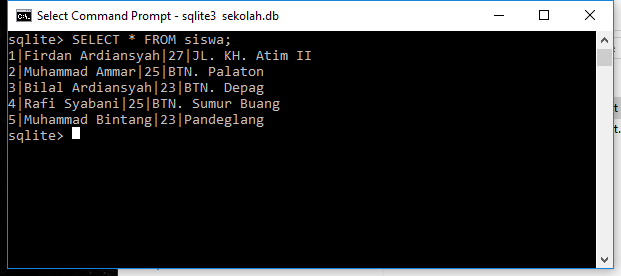
\includegraphics[width=1\textwidth]{figures/Sql.png}}
		\caption{Hasilnya}
		\label{Sql}
	\end{figure}
	Gambar \ref{Sql} Hasil gambar.
	
	\subsection{Fiture}
		\begin{enumerate}
			\item SQLite mengimplementasikan sebagian besar standar SQL-92 untuk SQL tetapi tidak memiliki beberapa fitur. Misalnya, beberapa menyediakan pemicu, dan tidak dapat menulis ke tampilan (tetapi menyediakan pemicu INSTEAD OF yang menyediakan fungsi ini). Meskipun menyediakan query kompleks, masih memiliki fungsi ALTER TABLE terbatas, karena tidak dapat memodifikasi atau menghapus kolom.
			\item SQLite menggunakan sistem tipe yang tidak biasa untuk DBMS yang kompatibel dengan SQL: alih-alih menetapkan jenis ke kolom seperti pada kebanyakan sistem basis data SQL, mereka ditetapkan ke nilai individual: dalam bahasa yang diketik secara dinamis. Selain itu, itu lemah diketik dalam beberapa cara yang sama bahwa Perl adalah: satu dapat memasukkan string ke dalam kolom integer (meskipun SQLite akan mencoba untuk mengubah string ke integer pertama, jika jenis kolom yang diinginkan adalah bilangan bulat). Ini menambah fleksibilitas ke kolom, terutama ketika terikat ke bahasa scripting yang diketik secara dinamis. Namun, teknik ini tidak portabel untuk produk SQL lainnya. Kritik umum adalah bahwa sistem tipe SQLite tidak memiliki mekanisme integritas data yang disediakan oleh kolom-kolom yang diketik secara statis dalam produk lain. Situs web SQLite menggambarkan mode afinitas yang ketat, tetapi fitur ini belum ditambahkan. Namun, itu dapat diimplementasikan dengan pembatasan semacam itu. Tabel biasanya menyertakan kolom index rowid tersembunyi yang memberikan akses lebih cepat. Jika database termasuk kolom Integer Primary Key, SQLite biasanya akan mengoptimalkannya dengan memperlakukannya sebagai alias untuk rowid, menyebabkan kontennya disimpan sebagai integer 64-bit yang diketik-ketat dan mengubah perilakunya menjadi agak seperti penambahan otomatis kolom. Versi masa depan dari SQLite mungkin termasuk perintah untuk mengintrospeksi apakah sebuah kolom memiliki perilaku seperti itu dari rowid untuk membedakan kolom ini dari Kunci Primer Integer yang tidak terkunci secara otomatis.
			\item SQLite dengan fungsi Unicode penuh adalah opsional.
			\item Beberapa proses komputer atau utas dapat mengakses basis data yang sama secara bersamaan. Beberapa akses dapat dibaca secara paralel. Akses hanya dapat digunakan jika ada. Jika tidak, akses tulis gagal dengan kode kesalahan (atau dapat dicoba kembali secara otomatis sampai batas waktu dapat dikonfigurasi untuk kedaluwarsa). Akses data ini akan berubah ketika berhadapan dengan tabel sementara. Pembatasan ini dilonggarkan dalam versi 3,7 dari kompilasi write-ahead (WAL) diaktifkan untuk memungkinkan membaca dan pencurian simultan. SQLite versi 3.7.4 pertama kali melihat modul FTS4 tambahan (pencarian teks lengkap), menampilkan perbaikan dalam modul FTS3 yang lebih lama. FTS4 memungkinkan pengguna untuk melakukan teks lengkap pada dokumen yang mirip dengan bagaimana mesin pencari mencari halaman web. Versi 3.8.2 Tambah untuk membuat tabel tanpa rowid, yang dapat memberikan ruang dan peningkatan kinerja. Penguatan tabel umum ditambahkan ke SQLite di versi 3.8.3.
		\end{enumerate}
	\subsection{Perkembangan dan Distribusi}
		\begin{enumerate}
			\item Kode SQLite di-host dengan Fossil, sistem kontrol versi terdistribusi yang dibangun di database SQLite.
			\item Program baris perintah yang berdiri sendiri disediakan dalam distribusi SQLite. Ini dapat digunakan untuk membuat database, menentukan tabel, menyisipkan dan mengubah baris, menjalankan kueri dan mengelola file database SQLite. Ini juga berfungsi sebagai contoh untuk menulis aplikasi yang menggunakan pustaka SQLite.
			\item SQLite menggunakan pengujian regresi otomatis sebelum setiap rilis. Lebih dari 2 juta tes dijalankan sebagai bagian dari verifikasi rilis. Dimulai dengan rilis 10 Agustus 2009 dari SQLite 3.6.17, rilis SQLite memiliki cakupan cabang cakupan 100%, salah satu komponen cakupan kode. Tes dan tes menggunakan domain publik dan kepemilikan parsial.
		\end{enumerate}
	\subsection{SQLite Serverless}
		\begin{enumerate}
			\item Sebagian besar mesin database SQL diimplementasikan sebagai proses server terpisah. Program yang ingin mengakses database berkomunikasi dengan server menggunakan beberapa jenis komunikasi interprocess (biasanya TCP / IP) untuk mengirim permintaan ke server dan menerima hasilnya kembali. SQLite tidak berfungsi dengan cara ini. Dengan SQLite, proses yang ingin mengakses database membaca dan menulis langsung dari file database pada disk. Tidak ada proses server menengah.
			\item Ada kelebihan dan kekurangan menjadi serverless. Keuntungan utama adalah tidak ada proses server terpisah untuk menginstal, mengkonfigurasi, mengkonfigurasi, menginisialisasi, mengelola, dan memecahkan masalah. Ini adalah salah satu alasan mengapa SQLite adalah mesin database "konfigurasi-nol". Program yang menggunakan SQLite tidak memerlukan dukungan administratif untuk menyiapkan mesin basis data sebelum dijalankan. Setiap program yang dapat mengakses disk dapat menggunakan database SQLite.
			\item Di sisi lain, mesin database yang menggunakan server dapat memberikan perlindungan yang lebih baik dari bug di aplikasi klien - pointer liar pada klien tidak dapat merusak memori di server. Dan karena server adalah proses persisten tunggal, ia mampu mengontrol akses basis data dengan lebih presisi, memungkinkan penguncian yang lebih baik dan konkurensi yang lebih baik.
			\item Sebagian besar mesin klien / server database berbasis SQL. Dari mereka tanpa server, SQLite adalah satu-satunya yang diketahui dari penulis ini yang memungkinkan beberapa aplikasi untuk mengakses database yang sama pada saat yang bersamaan.
			\item Biasanya, RDBMS seperti MySQL, PostgreSQL, dll, membutuhkan proses server terpisah untuk beroperasi. Aplikasi yang ingin mengakses server database menggunakan protokol TCP / IP untuk mengirim dan menerima permintaan. Ini disebut arsitektur client / server.
		\end{enumerate}
	\subsection{Neo Serverless vs Classic Serverless}
		\begin{enumerate}
			\item Baru-baru ini, orang mulai menggunakan kata serverless berarti sesuatu yang sangat berbeda dari makna yang dimaksudkan dalam dokumen ini. 
			\item Berikut dua definisi yang mungkin tanpa server:
			\item Classic Serverless: Mesin database berjalan dalam proses, thread, dan ruang alamat yang sama dengan aplikasi. Tidak ada pesan yang lewat atau aktivitas jaringan.
			\item Neo-Serverless: Mesin database berjalan di ruang nama aplikasi terpisah, mungkin pada mesin yang terpisah, tetapi database disediakan sebagai layanan turn-key oleh penyedia hosting, yang tidak memerlukan manajemen atau administrasi dari pemilik aplikasi, dan sangat mudah digunakan bahwa pengembang dapat mengasumsikan database sebagai serverless bahkan jika server benar-benar menggunakan di bawah selimut.
			\item SQLite adalah contoh mesin database tanpa server klasik. Dengan SQLite, tidak ada proses, thread, mesin, atau mekanisme lain (selain OS host komputer dan sistem file) untuk membantu menyediakan layanan atau implementasi database. Sama sekali tidak ada server.
			\item Microsoft Azure Cosmo DB dan Amazon S3 adalah contoh dari database neo-serverless. Database ini diimplementasikan oleh proses server yang berjalan secara terpisah di cloud. Tetapi server dikelola dan dikelola oleh ISP, bukan oleh pengembang aplikasi. Pengembang aplikasi hanya menggunakan layanan ini. Pengembang tidak harus menyediakan, mengkonfigurasi, atau mengelola instance server basis data, karena semua pekerjaan ditangani secara otomatis oleh penyedia layanan. Server database memang ada, mereka hanya tersembunyi dari para pengembang.
			\item Penting untuk memahami dua definisi yang berbeda ini untuk serverless. Ketika sebuah database mengklaim sebagai serverless, pastikan untuk mengetahui apakah itu berarti serverless klasik atau neo-serverless.
		\end{enumerate}
	\subsection{SQLite internal}
	\begin{enumerate}
	\item Bab ini adalah tur singkat melalui subsistem utama SQLite. Itu terinspirasi dari presentasi SQLite yang diberikan oleh Richard Hipp di konvensi yang saya hadiri. Sebagian besar materi yang disajikan di sini diambil langsung dari handout. Bahkan jika Anda tidak pernah melihat kode sumber SQLite, Anda mungkin menemukan materi dalam bab ini cukup menarik, seperti yang saya lakukan. Sementara beberapa materi cenderung berubah dengan perkembangan SQLite yang sedang berlangsung, konsep-konsep utama yang disajikan di sini tidak mungkin berubah terlalu dramatis.
	\end{enumerate}
		\subsection{Mandiri}
		\begin{enumerate}
		\item SQLite adalah alat mandiri yang memerlukan dukungan minimal dari sistem operasi atau pustaka eksternal. Ini membuat SQLite dapat digunakan di lingkungan apa pun terutama di perangkat yang tertanam seperti iPhone, ponsel Android, konsol game, pemutar media genggam, dll.
		\item SQLite dikembangkan menggunakan ANSI-C. Kode sumber tersedia sebagai sqlite3.c besar dan file header-nya sqlite3.h. Jika Anda ingin mengembangkan aplikasi yang menggunakan SQLite, Anda hanya perlu memasukkan file-file ini ke dalam proyek Anda dan kompilasi dengan kode Anda.
		\end{enumerate}
		
		\subsection{Kesimpulan}
			\begin{enumerate}
				\item SQLite adalah pusat dalam pemrosesan yang mengimplementasikan server di database SQL sendiri, tanpa server, nol - konfigurasii, transakssional. Kode untuk SQLite ada di domain publik dan dengan demikian bebas digunakan untuk tujuan apa pun, komersial atau pribadi. SQLite adalah database yang paling banyak digunakan di dunia dengan aplikasi lebih dari yang dapat kita hitung, termasuk beberapa proyek profil tinggi.
				\item SQLite adalah mesin basis data SQL tertanam. Tidak seperti kebanyakan database SQL lainnya, SQLite tidak memiliki proses server terpisah. SQLite membaca dan menulis langsung ke file disk biasa. Database SQL lengkap dengan banyak tabel, indeks, pemicu, dan tampilan, terdapat dalam satu file disk. Format file database adalah cross-platform - Anda dapat dengan bebas menyalin database antara sistem 32-bit dan 64-bit atau antara arsitektur big-endian dan little-endian. Fitur-fitur ini menjadikan SQLite pilihan populer sebagai Format File Aplikasi. Pikirkan SQLite bukan sebagai pengganti Oracle tetapi tidak fopen ().
				\item Karena arsitektur tanpa server, Anda tidak perlu "menginstal"Lite sebelum menggunakannya. Tidak ada proses server yang perlu dikonfigurasi, dimulai, dan dihentikan. elain itu, SQLite tidak menggunakan file konfigurasi apa pun.
				\item SQLite adalah pustaka yang ringkas. Dengan semua fitur diaktifkan, ukuran pustaka bisa kurang dari 500KiB, tergantung pada platform target dan pengaturan optimasi kompilator. (Kode 64-bit lebih besar, dan beberapa optimisasi kompilator seperti inlining fungsi agresif dan dekomposisi loop dapat menyebabkan kode objek menjadi jauh lebih besar.) Ada tradeoff antara penggunaan memori dan kecepatan. SQLite umumnya berjalan lebih cepat, semakin banyak memori yang Anda berikan. Namun demikian, kinerja biasanya cukup baik bahkan dalam lingkungan memori yang rendah. Tergantung pada bagaimana itu digunakan, SQLite bisa lebih cepat daripada filesystem langsung I atau O.
				\item SQLite sangat hati-hati diuji sebelum rilis masing-masing dan memiliki reputasi sebagai sangat dapat diandalkan. Sebagian besar kode sumber SQLite spesifik untuk pengujian dan verifikasi. Sebuah rangkaian uji otomatis menjalankan jutaan dan jutaan kasus uji coba yang melibatkan ratusan juta pernyataan SQL individual dan mencapai cakupan cakupan 100%. SQLite merespon dengan anggun untuk kegagalan alokasi memori dan disk I / O kesalahan. Transaksi adalah ACID bahkan jika terganggu oleh sistem crash atau gangguan listrik. Semua ini diverifikasi oleh tes otomatis menggunakan alat uji khusus yang mensimulasikan kegagalan sistem. Tentu saja, bahkan dengan semua tes ini, masih ada bug. Tapi tidak seperti beberapa proyek serupa (terutama pesaing komersial) SQLite terbuka dan jujur ​​tentang semua bug dan memberikan daftar bug dan kronologi menit-demi-menit dari perubahan kode.
				\item Basis kode SQLite didukung oleh tim pengembangan internasional yang bekerja pada SQLite penuh waktu. Pengembang terus memperluas kemampuan SQLite dan meningkatkan keandalan dan kinerja mereka sambil mempertahankan kompatibilitas mundur dengan spesifikasi antarmuka yang dipublikasikan, sintaks SQL, dan format file database. Kode sumbernya benar-benar gratis bagi siapa saja yang menginginkannya, tetapi dukungan profesional juga tersedia.
				\item SQLite menggunakan tipe dinamis untuk tabel. Ini berarti Anda dapat menyimpan nilai apa pun di kolom mana pun, apa pun jenis datanya. SQLite memungkinkan koneksi database tunggal untuk mengakses beberapa file database secara bersamaan. Ini membawa banyak fitur bagus seperti menggabungkan tabel di database yang berbeda atau menyalin data antar database dalam satu perintah tunggal. SQLite mampu menciptakan database di-memori yang sangat cepat untuk bekerja.
				\item Semua transaksi dalam SQLite sepenuhnya mematuhi ACID. Ini berarti semua pertanyaan dan perubahan adalah Atom, Konsisten, Terisolasi, dan Tahan Lama. Dengan kata lain, semua perubahan dalam transaksi terjadi sepenuhnya atau bahkan ketika situasi tak terduga seperti aplikasi macet, kegagalan daya, atau terjadi crash sistem operasi.
				\item Proyek SQLite dimulai pada 2000-05-09. Masa depan selalu tidak dapat diprediksi, tetapi maksud dari pengembang adalah untuk mendukung SQLite sepanjang tahun 2050. Keputusan desain dibuat dengan mengingat tujuan tersebut.
				\item Kami pengembang berharap bahwa Anda menemukan SQLite berguna dan kami meminta Anda untuk menggunakannya dengan baik: untuk membuat produk cantik dan indah yang cepat, andal, dan mudah digunakan. Carilah pengampunan untuk diri sendiri saat Anda memaafkan orang lain. Dan sama seperti Anda telah menerima SQLite gratis, jadi berikan juga gratis, bayar utang ke depan.

			\end{enumerate}
			


\cite{owens2010sqlite}
\cite{newman2004sqlite}
\cite{kreibich2010using}
\cite{kang2013x}
\cite{jeon2012recovery}
\cite{lee2012creating}

\subsection{insert sqlite language}
\begin{enumerate}
\itemSisipan Bahasa Query Sqlite
Pernyataan INSERT hadir dalam tiga bentuk dasar.
1. INSERT INTO table VALUES (...);
Bentuk pertama (dengan kata kunci "VALUES") membuat satu atau lebih baris baru dalam tabel yang ada. Jika daftar nama kolom setelah nama tabel dihilangkan, maka jumlah nilai yang dimasukkan ke setiap baris harus sama dengan jumlah kolom dalam tabel. Dalam hal ini, hasil evaluasi ekspresi paling kiri dari setiap istilah daftar VALUES dimasukkan ke dalam kolom paling kiri dari setiap baris baru, dan seterusnya untuk setiap ekspresi berikutnya. Jika daftar kolom-nama ditentukan, maka jumlah nilai dalam setiap jangka waktu daftar VALUE harus sesuai dengan jumlah kolom yang ditentukan. Setiap kolom bernama dari baris baru diisi dengan hasil mengevaluasi ekspresi VALUES yang sesuai. Kolom tabel yang tidak muncul dalam daftar kolom diisi dengan nilai kolom default (ditetapkan sebagai bagian dari pernyataan CREATE TABLE), atau dengan NULL jika tidak ada nilai default yang ditentukan.
2. INSERT INTO table SELECT ...;
Bentuk kedua dari pernyataan INSERT berisi pernyataan SELECT bukannya klausa VALUES. Entri baru dimasukkan ke dalam tabel untuk setiap baris data yang dikembalikan dengan mengeksekusi pernyataan SELECT. Jika daftar kolom ditentukan, jumlah kolom dalam hasil SELECT harus sama dengan jumlah item dalam daftar-kolom. Jika tidak, jika tidak ada daftar kolom yang ditentukan, jumlah kolom dalam hasil SELECT harus sama dengan jumlah kolom dalam tabel. Setiap pernyataan SELECT, termasuk pernyataan gabungan SELECT dan SELECT dengan klausa ORDER BY dan / atau LIMIT, dapat digunakan dalam pernyataan INSERT dari formulir ini.
3. INSERT INTO table DEFAULT VALUES;
Bentuk ketiga dari pernyataan INSERT adalah dengan NILAI DEFAULT. Pernyataan INSERT ... DEFAULT VALUES menyisipkan satu baris baru ke dalam tabel bernama. Setiap kolom dari baris baru diisi dengan nilai default-nya, atau dengan NULL jika tidak ada nilai default yang ditetapkan sebagai bagian dari definisi kolom dalam pernyataan CREATE TABLE.
\end{enumerate}
			
			



%\chapter[DeadLock]
%{OS\\ DeadLock}
%%Nama Kelompok: Sistem_Operasi_Deadlock
%Kelas: D4 TI 1B
%Alit Fajar Kurniawan(1174057) 
%Muhammad Iqbal Panggabean(1174063)
%Muhammad Afra Faris(1174041)
%Khadijah Hasanah Puteri Harahap(1174044)

\section {DEADLOCK}

\subsection {Deadlock}
\subsubsection {Pengertian Deadlock}
	Pada kesempatan ini saya akan menjelaskan tentang definisi Deadlock, Deadlock ialah suatu keadaan yang dimana dua proses atau lebih, saling menunggu proses untuk dapat melepaskan sumber daya yang sedang dijalankan. Misalnya proses A yang memperlukan suatu sumber daya, tetapi sumber saya tersebut sedang digunkana oleh proses lain. Untuk lebih paham mengenai pengertian dari deadlock dan bagaimana cara mengatasinya, anda dapat membandingkannya dengan situasi yang satu ini. Pertama, Dalam kehidupan kita tentu membutuhkan suatu pekerjaan, dan untuk memperoleh suatu pekerjaan, anda harus memiliki pengalaman yang baik, untuk dapat memiliki pengalaman yang baik anda harus bekerja.

	\begin{figure}[ht]
	\centerline{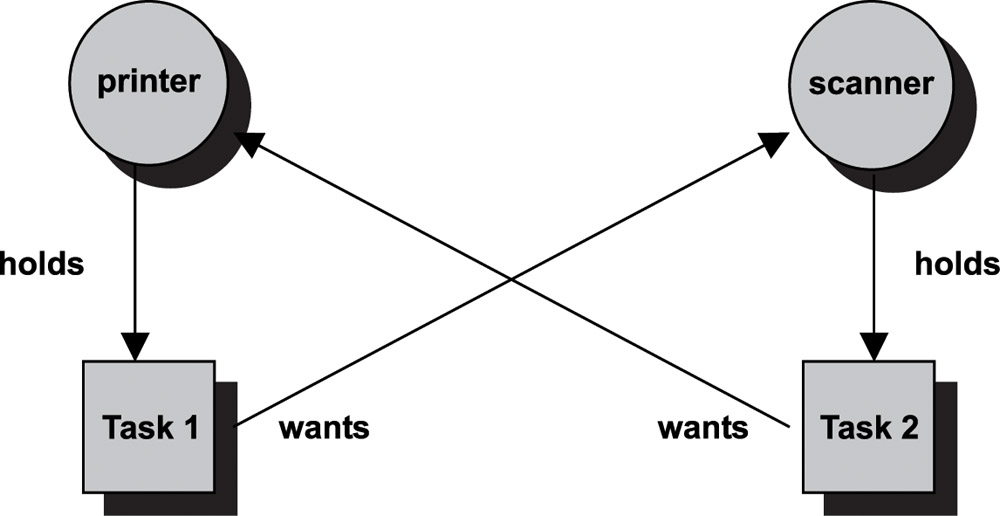
\includegraphics[width=1\textwidth]{figures/deadlock1.jpg}}
	\caption{Gambar Deadlock}
	\label{Gambar}
	\end{figure}
      
      Gambar \ref{Gambar_Deadlock} Contoh gambar pada saat terjadinya deadlock.

\subsection {Masalah Deadlock dan Metode Penanganan Deadlock}
\subsubsection {Masalah Deadlock}
	Deadlock merupakan dampak pengaruh dari sinkronisasi, yaitu dimana satu variabel yang digunakan oleh dua proses yang berbeda. Deadlock selalu tidak terlepas dari yang namanya sumber daya, karena hampir secara keseluruhan merupakan masalah mengenai sebuah sumber daya yang digunakan secara bersamaan. Sebuah Kelompok Proses yang diblok atau diblokir, dimana setiap proses memegang sebuah resource dan kemudian menunggu resource lain dari proses yang berada didalam proses yang sedang diBlok tersebut, biasanya dari semua proses-proses atau resource yang non preemptive.
	
\subsubsection {Metode Penanganan}
	Ada tiga Metode penanganan Deadlock:
	Yang Pertama yaitu, anda harus menggunakan satu protokol yang dapat membuat anda yakin bahwa sistem tersebut tidak akan pernah mengalami kejadian deadlock. Metode ini bisa disebut dengan Deadlock Prevention atau Avoidance.
	
	Yang Kedua, anda harus memberikan izin sistem untuk mengalami kejadian deadlock, namun setelah terjadinya deadlock anda harus dengan cepat segera untuk memperbaiki sistem yang mengalami deadlock tersebut. Metode ini biasanya disebut dengan Deadlock detection and recovery.
	
	Dan yang terakhir, anda hanya mengabaikan semua permasalahan yang terjadi secara bersamaan, dan kemudian menganggap bahwa deadlock tidak akan terjadi, metode ini digunakan dalam berbagai sistem operasi komputer, termasuk windows dan unix.

\begin{table}[H]
\begin{tabular}{|c|c|c|c|c|}
hline
Proses & Jumlah Sumber Daya Digenggam & Maksimum Sumber Daya Dibutuhkan\\
\hline
X   & 2 & 10\\
Y   & 1 & 3\\
Z   & 3 & 7\\
\hline
Tersedia 4
\hline
\end{tabular}
\end{table}

\subsection {Deadlock Detection}
\begin {enumerate}
\item
1. Pendeteksian secara Algoritma, yaitu dengan cara kita mengetahui jika terjadinya deadlock, deadlock terjadi jika suatu permintaan tidak dapat ditangani segera.
	
\item
2. Recovery atau Pemulihan, yaitu yang pertama menggagalkan semua proses deadlock, yang kedua mem backup semua proses yang deadlock dan kemudian silahkan melakukan restart di semua proses yang sedang terjadi, yang ketiga menggagalkan semua proses yang deadlock secara berurutan sehingga tidak akan terjadi lagi deadock, dan yang terakhir yaitu menggagalkan pengalokasian resource secara berurutan hingga tidak ada deadlock.

\end {enumerate}

\subsection {Beberapa hal yang terjadi ketika mendeteksi adanya deadlock}
\begin {enumerate}
\item
1. Permintaan sumber daya dikabulkan selama memungkinkan.
\item
2. Sistem operasi melakukan scanning apakah ada kondisi circular wait secara peiodik.
\item
3. Pemeriksaan dilakukan setiap ada sumber daya yang hendak digunakan.
\item
4. memeriksa dengan algoritma tertentu.
\end {enumerate}

\subsection {Beberapa jalan untuk kembali dari deadlock}
\begin {enumerate}
\item
1. Lewat Preemption, yaitu dengan jauhkan sumber daya dari pemakainya untuk sementara waktu, tujuannya untuk memberikannya pada proses lain. strategi dengan memberikannya kesempatan pada proses lain dengan tanpa diketahui oleh pemilik dari sumber daya itu dan tergantung juga dari sifat sumber daya itu sendiri.
\item
2. Lewat melacak kembali, setelah melakukan prosesn dari preemption tersebut maka secara otomatis proses utama yang diambil sumber dayanya akan stop dan tidak akan melanjutkan prosesnya, oleh karena itu dibutuhkan langkah untuk dapat kembali pada keadaan aman, tetapi untuk menentukan keadaan aman tersebut sangatlah susah.
\item
3. Mematikan proses yang menyebabkan deadlock, ini merupakan cara yang sangat umum digunakan yaitu dengan cara mematikan semua proses yang mengalami deadlock.
\item
4. Menghindari deadlock, pada sistem permintaan untuk sumberdaya biasanya hanya dilakukan sekali saja, sistem harus sudah dapat mengenali bahwa sistem itu aman atau tidak.
\end {enumerate}

\subsection {Reference}

@article{siahaan2015penyelarasan,
  title={Penyelarasan Pada Masalah Dining Philosophers Menggunakan Algoritma Lock \& Release},
  author={Siahaan, Andysah Putera Utama},
  journal={TECHSI-Jurnal Teknik Informatika},
  volume={7},
  number={1},
  year={2015}
}

@article{fauzi2013perangkat,
  title={PERANGKAT LUNAK VISUALISASI PERJALANAN KERETA API DENGAN MENGGUNAKAN PENDEKATAN SEMAPHORE, DEADLOCK SOLUTION DAN ALGORITMA DIJKSTRA},
  author={Fauzi, Esa},
  year={2013},
  publisher={Universitas Widyatama}
}

@book{silberschatz2014operating,
  title={Operating system concepts essentials},
  author={Silberschatz, Abraham and Galvin, Peter Baer and Gagne, Greg},
  year={2014},
  publisher={John Wiley \& Sons, Inc.}
}


%\chapter[Internet]
%{Definisi\\ Internet}
%\input{section/1internet.tex}

%\chapter[Web]
%{Definisi\\ Web}
%\input{section/1web.tex}

%\chapter[Backend]
%{Definisi\\ Backend}
%\input{section/1Backend.tex}

%\chapter[Frontend]
%{Definisi\\ Frontend}
%\input{section/1Frontend.tex}

% contoh aplikasi web service
% web service
% protokol
% port

% HTTP
% URL
% POST
% GET


\bibliographystyle{IEEEtran}
\bibliography{references, kelompok31A}

\printindex

\end{document}

